\documentclass[11pt]{article}
\usepackage[T1]{fontenc}
\usepackage[utf8]{inputenc}
\usepackage[a4paper,margin=2.2cm]{geometry}
\usepackage{amsmath,amssymb}
\DeclareUnicodeCharacter{2212}{-}
\usepackage{enumitem}
\usepackage{xcolor}
\usepackage{tikz}
\usepackage{pgfplots}
\pgfplotsset{compat=1.17}
\usetikzlibrary{calc}
\usepackage[colorlinks=true,linkcolor=blue!60!black,urlcolor=blue]{hyperref}

% ---- question / answer boxes (no external dependency) -------------------
\newenvironment{qbox}{%
  \par\smallskip\noindent
  
\begin{tikzpicture}\node[draw=blue!55!black,fill=blue!4,rounded corners=3pt,
    inner sep=8pt,text width=\dimexpr\linewidth-20pt\relax]\bgroup}%
  {\egroup;\end{tikzpicture}\par\smallskip}
\newenvironment{ansbox}{%
  \par\smallskip\noindent
  
\begin{tikzpicture}\node[draw=green!45!black,fill=green!6,rounded corners=3pt,
    inner sep=7pt,text width=\dimexpr\linewidth-20pt\relax]\bgroup}%
  {\egroup;\end{tikzpicture}\par\smallskip}

\setlength{\parindent}{0pt}
\setlength{\parskip}{4pt}

\title{\textbf{Factorising Quadratics}\\[4pt]\large Complete Worked Solutions with Diagrams}
\author{Wisest Maths --- Year 1 A-Level (topic ref: \texttt{qc1})}
\date{Generated automatically from the question bank}
\begin{document}
\maketitle
\thispagestyle{empty}

\section*{About this document}
This booklet contains every question from the \textbf{Factorising Quadratics} bank
(\texttt{qc1-001} to \texttt{qc1-070}), each presented with a full step-by-step worked
solution, a check by expansion, and supporting diagrams drawn in Ti\emph{k}Z:
\begin{itemize}[leftmargin=1.4em]
  \item an \textbf{area / box model}, where every cell is the product of its row and
        column term --- the four (or more) cells sum to the original quadratic; and
  \item for numeric examples, a \textbf{graph} $y=f(x)$ showing the parabola together
        with its roots (where it crosses the $x$-axis) and its vertex.
\end{itemize}
The box model makes the link between \emph{factorising} (splitting a rectangle into pieces)
and \emph{expanding} (recombining them) explicit, while the graph connects the algebra to
the geometry of the curve.

\vspace{6pt}\hrule
\tableofcontents
\newpage

\section*{Question 1 \quad {\normalfont\small\ttfamily qc1-001}}
\addcontentsline{toc}{section}{Q1. Monic ($a=1$)}
\nopagebreak
\begin{qbox}
Factorise: \( x^2 + 5x + 6 \)
\end{qbox}
\smallskip\noindent\textit{Type:} Monic ($a=1$) \hfill \textit{Marks:} 2 \quad \textit{Difficulty:} Foundation\\[2pt]
\subsection*{Worked solution}
\begin{enumerate}[leftmargin=1.6em,label=\textbf{Step \arabic*.}]
  \item Write down two brackets, each starting with \( x \).
  \[ (x \quad )(x \quad ) \]
  \par\smallskip{\small\itshape Since the leading coefficient is 1, both brackets begin with \( x \).}
  \item Find two numbers that multiply to give \( +6 \) and add to give \( +5 \).
  \[ 2 \times 3 = 6, \quad 2 + 3 = 5 \]
  \par\smallskip{\small\itshape The pair \( (2, 3) \) works for both conditions.}
  \item Place the numbers into the brackets.
  \[ (x + 2)(x + 3) \]
  \par\smallskip{\small\itshape Both signs are positive because c and b are positive.}
\end{enumerate}
\begin{ansbox}\textbf{Final answer:}\quad \((x + 2)(x + 3)\)\end{ansbox}
\subsection*{Check by expanding}
Multiplying the brackets back out reproduces the original expression:
\[ x^{2} +3x +2x +6 \]
\subsection*{Visualising the factorisation}
\begin{center}
\begin{tabular}{cc}
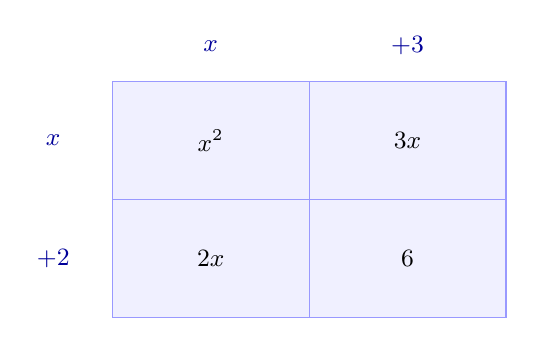
\begin{tikzpicture}[font=\small]
  \fill[blue!6] (0,0) rectangle (2.5,-1.5);
  \draw[blue!40] (0,0) rectangle (2.5,-1.5);
  \node at (1.25,-0.75) {$x^{2}$};
  \fill[blue!6] (2.5,0) rectangle (5,-1.5);
  \draw[blue!40] (2.5,0) rectangle (5,-1.5);
  \node at (3.75,-0.75) {$3x$};
  \fill[blue!6] (0,-1.5) rectangle (2.5,-3);
  \draw[blue!40] (0,-1.5) rectangle (2.5,-3);
  \node at (1.25,-2.25) {$2x$};
  \fill[blue!6] (2.5,-1.5) rectangle (5,-3);
  \draw[blue!40] (2.5,-1.5) rectangle (5,-3);
  \node at (3.75,-2.25) {$6$};
  \node[blue!60!black] at (1.25,0.45) {$x$};
  \node[blue!60!black] at (3.75,0.45) {$+3$};
  \node[blue!60!black] at (-0.75,-0.75) {$x$};
  \node[blue!60!black] at (-0.75,-2.25) {$+2$};
\end{tikzpicture} &
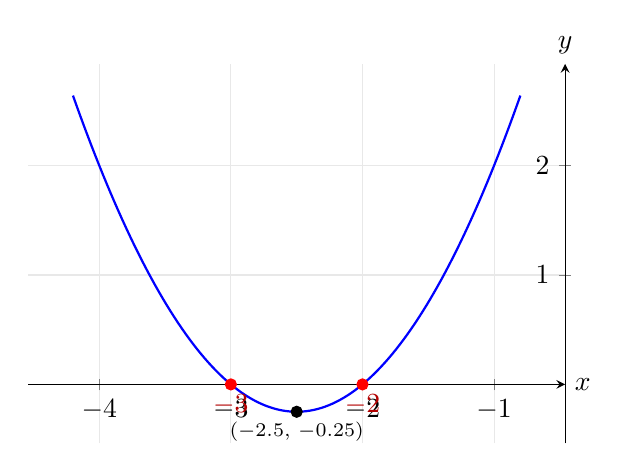
\begin{tikzpicture}
\begin{axis}[
  axis lines=middle, xlabel={$x$}, ylabel={$y$},
  width=8.4cm, height=6.4cm, grid=both, grid style={gray!18},
  enlargelimits=true, samples=120,
  domain=-4.2:-0.8, every axis x label/.style={at={(ticklabel* cs:1)},anchor=west},
  every axis y label/.style={at={(ticklabel* cs:1)},anchor=south}]
  \addplot[blue, thick]{1*x^2 + 5*x + 6};
  \addplot[only marks, mark=*, red] coordinates {(-2,0)};
  \node[red!70!black, anchor=north] at (axis cs:-2,0) {$-2$};
  \addplot[only marks, mark=*, red] coordinates {(-3,0)};
  \node[red!70!black, anchor=north] at (axis cs:-3,0) {$-3$};
  \addplot[only marks, mark=*, black] coordinates {(-2.5,-0.25)};
  \node[anchor=north] at (axis cs:-2.5,-0.25) {\scriptsize $(-2.5,\,-0.25)$};
\end{axis}
\end{tikzpicture}
\\[4pt]
{\small (a) Area / box model} & {\small (b) Graph $y=f(x)$ with its roots} \\
\end{tabular}
\end{center}
\vspace{2pt}\hrule\vspace{6pt}

\section*{Question 2 \quad {\normalfont\small\ttfamily qc1-002}}
\addcontentsline{toc}{section}{Q2. Monic ($a=1$)}
\nopagebreak
\begin{qbox}
Factorise: \( x^2 + 7x + 12 \)
\end{qbox}
\smallskip\noindent\textit{Type:} Monic ($a=1$) \hfill \textit{Marks:} 2 \quad \textit{Difficulty:} Foundation\\[2pt]
\subsection*{Worked solution}
\begin{enumerate}[leftmargin=1.6em,label=\textbf{Step \arabic*.}]
  \item Set up two brackets starting with \( x \).
  \[ (x \quad )(x \quad ) \]
  \par\smallskip{\small\itshape The leading term is \( x^2 \), so both brackets begin with \( x \).}
  \item Find two numbers that multiply to 12 and add to 7.
  \[ 3 \times 4 = 12, \quad 3 + 4 = 7 \]
  \par\smallskip{\small\itshape Factor pairs of 12 are (1,12), (2,6), (3,4). Only (3,4) adds to 7.}
  \item Write the factorised form.
  \[ (x + 3)(x + 4) \]
  \par\smallskip{\small\itshape Both signs are positive.}
\end{enumerate}
\begin{ansbox}\textbf{Final answer:}\quad \((x + 3)(x + 4)\)\end{ansbox}
\subsection*{Check by expanding}
Multiplying the brackets back out reproduces the original expression:
\[ x^{2} +4x +3x +12 \]
\subsection*{Visualising the factorisation}
\begin{center}
\begin{tabular}{cc}
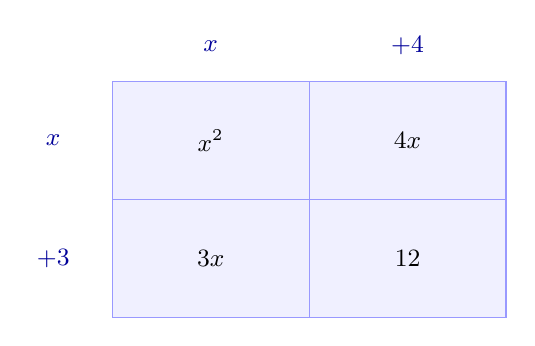
\begin{tikzpicture}[font=\small]
  \fill[blue!6] (0,0) rectangle (2.5,-1.5);
  \draw[blue!40] (0,0) rectangle (2.5,-1.5);
  \node at (1.25,-0.75) {$x^{2}$};
  \fill[blue!6] (2.5,0) rectangle (5,-1.5);
  \draw[blue!40] (2.5,0) rectangle (5,-1.5);
  \node at (3.75,-0.75) {$4x$};
  \fill[blue!6] (0,-1.5) rectangle (2.5,-3);
  \draw[blue!40] (0,-1.5) rectangle (2.5,-3);
  \node at (1.25,-2.25) {$3x$};
  \fill[blue!6] (2.5,-1.5) rectangle (5,-3);
  \draw[blue!40] (2.5,-1.5) rectangle (5,-3);
  \node at (3.75,-2.25) {$12$};
  \node[blue!60!black] at (1.25,0.45) {$x$};
  \node[blue!60!black] at (3.75,0.45) {$+4$};
  \node[blue!60!black] at (-0.75,-0.75) {$x$};
  \node[blue!60!black] at (-0.75,-2.25) {$+3$};
\end{tikzpicture} &
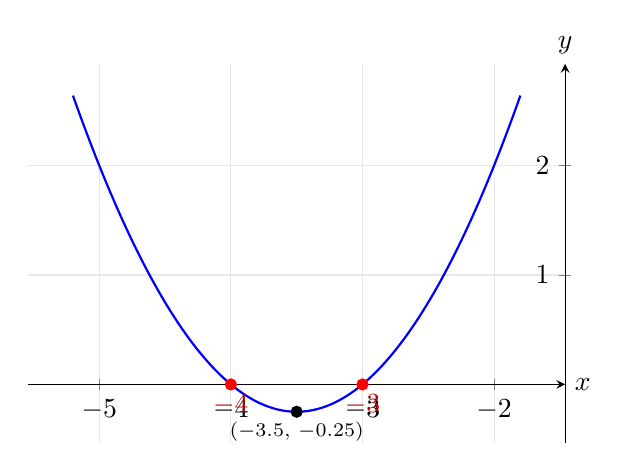
\begin{tikzpicture}
\begin{axis}[
  axis lines=middle, xlabel={$x$}, ylabel={$y$},
  width=8.4cm, height=6.4cm, grid=both, grid style={gray!18},
  enlargelimits=true, samples=120,
  domain=-5.2:-1.8, every axis x label/.style={at={(ticklabel* cs:1)},anchor=west},
  every axis y label/.style={at={(ticklabel* cs:1)},anchor=south}]
  \addplot[blue, thick]{1*x^2 + 7*x + 12};
  \addplot[only marks, mark=*, red] coordinates {(-3,0)};
  \node[red!70!black, anchor=north] at (axis cs:-3,0) {$-3$};
  \addplot[only marks, mark=*, red] coordinates {(-4,0)};
  \node[red!70!black, anchor=north] at (axis cs:-4,0) {$-4$};
  \addplot[only marks, mark=*, black] coordinates {(-3.5,-0.25)};
  \node[anchor=north] at (axis cs:-3.5,-0.25) {\scriptsize $(-3.5,\,-0.25)$};
\end{axis}
\end{tikzpicture}
\\[4pt]
{\small (a) Area / box model} & {\small (b) Graph $y=f(x)$ with its roots} \\
\end{tabular}
\end{center}
\vspace{2pt}\hrule\vspace{6pt}

\section*{Question 3 \quad {\normalfont\small\ttfamily qc1-003}}
\addcontentsline{toc}{section}{Q3. Monic ($a=1$)}
\nopagebreak
\begin{qbox}
Factorise: \( x^2 + 9x + 20 \)
\end{qbox}
\smallskip\noindent\textit{Type:} Monic ($a=1$) \hfill \textit{Marks:} 2 \quad \textit{Difficulty:} Foundation\\[2pt]
\subsection*{Worked solution}
\begin{enumerate}[leftmargin=1.6em,label=\textbf{Step \arabic*.}]
  \item Set up the two brackets.
  \[ (x \quad )(x \quad ) \]
  \par\smallskip{\small\itshape Leading coefficient is 1.}
  \item Find two numbers multiplying to 20 and adding to 9.
  \[ 4 \times 5 = 20, \quad 4 + 5 = 9 \]
  \par\smallskip{\small\itshape Factor pairs of 20: (1,20), (2,10), (4,5). Only (4,5) adds to 9.}
  \item Write the factors.
  \[ (x + 4)(x + 5) \]
  \par\smallskip{\small\itshape Both positive.}
\end{enumerate}
\begin{ansbox}\textbf{Final answer:}\quad \((x + 4)(x + 5)\)\end{ansbox}
\subsection*{Check by expanding}
Multiplying the brackets back out reproduces the original expression:
\[ x^{2} +5x +4x +20 \]
\subsection*{Visualising the factorisation}
\begin{center}
\begin{tabular}{cc}
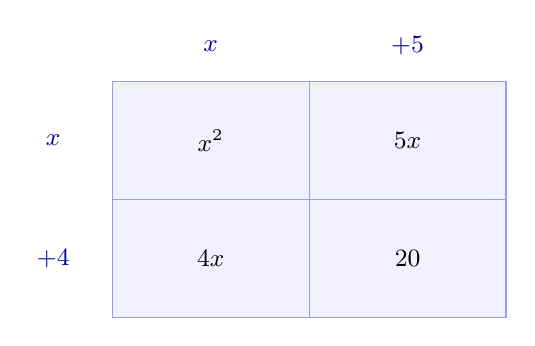
\begin{tikzpicture}[font=\small]
  \fill[blue!6] (0,0) rectangle (2.5,-1.5);
  \draw[blue!40] (0,0) rectangle (2.5,-1.5);
  \node at (1.25,-0.75) {$x^{2}$};
  \fill[blue!6] (2.5,0) rectangle (5,-1.5);
  \draw[blue!40] (2.5,0) rectangle (5,-1.5);
  \node at (3.75,-0.75) {$5x$};
  \fill[blue!6] (0,-1.5) rectangle (2.5,-3);
  \draw[blue!40] (0,-1.5) rectangle (2.5,-3);
  \node at (1.25,-2.25) {$4x$};
  \fill[blue!6] (2.5,-1.5) rectangle (5,-3);
  \draw[blue!40] (2.5,-1.5) rectangle (5,-3);
  \node at (3.75,-2.25) {$20$};
  \node[blue!60!black] at (1.25,0.45) {$x$};
  \node[blue!60!black] at (3.75,0.45) {$+5$};
  \node[blue!60!black] at (-0.75,-0.75) {$x$};
  \node[blue!60!black] at (-0.75,-2.25) {$+4$};
\end{tikzpicture} &
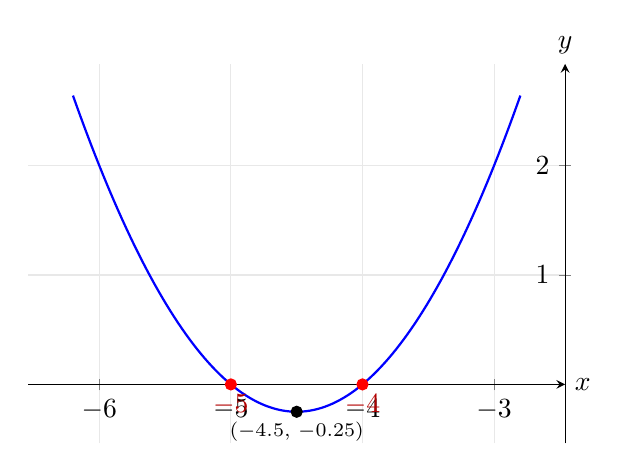
\begin{tikzpicture}
\begin{axis}[
  axis lines=middle, xlabel={$x$}, ylabel={$y$},
  width=8.4cm, height=6.4cm, grid=both, grid style={gray!18},
  enlargelimits=true, samples=120,
  domain=-6.2:-2.8, every axis x label/.style={at={(ticklabel* cs:1)},anchor=west},
  every axis y label/.style={at={(ticklabel* cs:1)},anchor=south}]
  \addplot[blue, thick]{1*x^2 + 9*x + 20};
  \addplot[only marks, mark=*, red] coordinates {(-4,0)};
  \node[red!70!black, anchor=north] at (axis cs:-4,0) {$-4$};
  \addplot[only marks, mark=*, red] coordinates {(-5,0)};
  \node[red!70!black, anchor=north] at (axis cs:-5,0) {$-5$};
  \addplot[only marks, mark=*, black] coordinates {(-4.5,-0.25)};
  \node[anchor=north] at (axis cs:-4.5,-0.25) {\scriptsize $(-4.5,\,-0.25)$};
\end{axis}
\end{tikzpicture}
\\[4pt]
{\small (a) Area / box model} & {\small (b) Graph $y=f(x)$ with its roots} \\
\end{tabular}
\end{center}
\vspace{2pt}\hrule\vspace{6pt}

\section*{Question 4 \quad {\normalfont\small\ttfamily qc1-004}}
\addcontentsline{toc}{section}{Q4. Monic ($a=1$)}
\nopagebreak
\begin{qbox}
Factorise: \( x^2 + 11x + 24 \)
\end{qbox}
\smallskip\noindent\textit{Type:} Monic ($a=1$) \hfill \textit{Marks:} 2 \quad \textit{Difficulty:} Foundation\\[2pt]
\subsection*{Worked solution}
\begin{enumerate}[leftmargin=1.6em,label=\textbf{Step \arabic*.}]
  \item Write down two brackets beginning with \( x \).
  \[ (x \quad )(x \quad ) \]
  \par\smallskip{\small\itshape Monic quadratic.}
  \item Find two numbers multiplying to 24 and adding to 11.
  \[ 3 \times 8 = 24, \quad 3 + 8 = 11 \]
  \par\smallskip{\small\itshape Factor pairs of 24: (1,24),(2,12),(3,8),(4,6). Only (3,8) sums to 11.}
  \item Write the answer.
  \[ (x + 3)(x + 8) \]
  \par\smallskip{\small\itshape Both signs positive.}
\end{enumerate}
\begin{ansbox}\textbf{Final answer:}\quad \((x + 3)(x + 8)\)\end{ansbox}
\subsection*{Check by expanding}
Multiplying the brackets back out reproduces the original expression:
\[ x^{2} +8x +3x +24 \]
\subsection*{Visualising the factorisation}
\begin{center}
\begin{tabular}{cc}
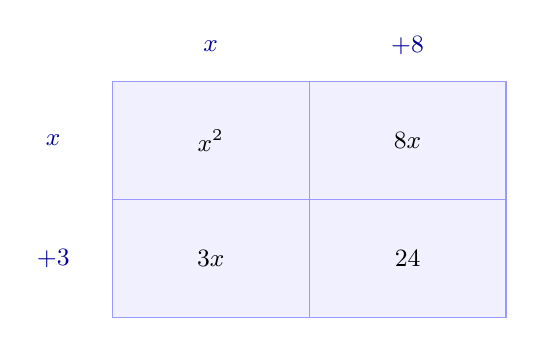
\begin{tikzpicture}[font=\small]
  \fill[blue!6] (0,0) rectangle (2.5,-1.5);
  \draw[blue!40] (0,0) rectangle (2.5,-1.5);
  \node at (1.25,-0.75) {$x^{2}$};
  \fill[blue!6] (2.5,0) rectangle (5,-1.5);
  \draw[blue!40] (2.5,0) rectangle (5,-1.5);
  \node at (3.75,-0.75) {$8x$};
  \fill[blue!6] (0,-1.5) rectangle (2.5,-3);
  \draw[blue!40] (0,-1.5) rectangle (2.5,-3);
  \node at (1.25,-2.25) {$3x$};
  \fill[blue!6] (2.5,-1.5) rectangle (5,-3);
  \draw[blue!40] (2.5,-1.5) rectangle (5,-3);
  \node at (3.75,-2.25) {$24$};
  \node[blue!60!black] at (1.25,0.45) {$x$};
  \node[blue!60!black] at (3.75,0.45) {$+8$};
  \node[blue!60!black] at (-0.75,-0.75) {$x$};
  \node[blue!60!black] at (-0.75,-2.25) {$+3$};
\end{tikzpicture} &
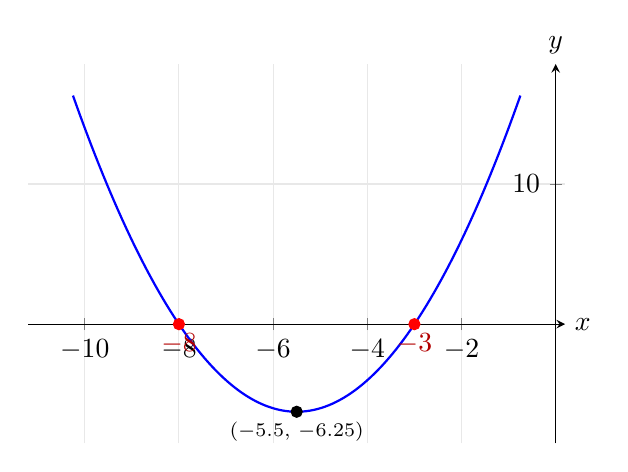
\begin{tikzpicture}
\begin{axis}[
  axis lines=middle, xlabel={$x$}, ylabel={$y$},
  width=8.4cm, height=6.4cm, grid=both, grid style={gray!18},
  enlargelimits=true, samples=120,
  domain=-10.25:-0.75, every axis x label/.style={at={(ticklabel* cs:1)},anchor=west},
  every axis y label/.style={at={(ticklabel* cs:1)},anchor=south}]
  \addplot[blue, thick]{1*x^2 + 11*x + 24};
  \addplot[only marks, mark=*, red] coordinates {(-3,0)};
  \node[red!70!black, anchor=north] at (axis cs:-3,0) {$-3$};
  \addplot[only marks, mark=*, red] coordinates {(-8,0)};
  \node[red!70!black, anchor=north] at (axis cs:-8,0) {$-8$};
  \addplot[only marks, mark=*, black] coordinates {(-5.5,-6.25)};
  \node[anchor=north] at (axis cs:-5.5,-6.25) {\scriptsize $(-5.5,\,-6.25)$};
\end{axis}
\end{tikzpicture}
\\[4pt]
{\small (a) Area / box model} & {\small (b) Graph $y=f(x)$ with its roots} \\
\end{tabular}
\end{center}
\vspace{2pt}\hrule\vspace{6pt}

\section*{Question 5 \quad {\normalfont\small\ttfamily qc1-005}}
\addcontentsline{toc}{section}{Q5. Monic ($a=1$)}
\nopagebreak
\begin{qbox}
Factorise: \( x^2 + 10x + 21 \)
\end{qbox}
\smallskip\noindent\textit{Type:} Monic ($a=1$) \hfill \textit{Marks:} 2 \quad \textit{Difficulty:} Foundation\\[2pt]
\subsection*{Worked solution}
\begin{enumerate}[leftmargin=1.6em,label=\textbf{Step \arabic*.}]
  \item Set up two brackets.
  \[ (x \quad )(x \quad ) \]
  \par\smallskip{\small\itshape Leading coefficient is 1.}
  \item Find numbers multiplying to 21 and adding to 10.
  \[ 3 \times 7 = 21, \quad 3 + 7 = 10 \]
  \par\smallskip{\small\itshape Factor pairs of 21: (1,21),(3,7). (3,7) works.}
  \item Write the answer.
  \[ (x + 3)(x + 7) \]
  \par\smallskip{\small\itshape Both signs positive.}
\end{enumerate}
\begin{ansbox}\textbf{Final answer:}\quad \((x + 3)(x + 7)\)\end{ansbox}
\subsection*{Check by expanding}
Multiplying the brackets back out reproduces the original expression:
\[ x^{2} +7x +3x +21 \]
\subsection*{Visualising the factorisation}
\begin{center}
\begin{tabular}{cc}
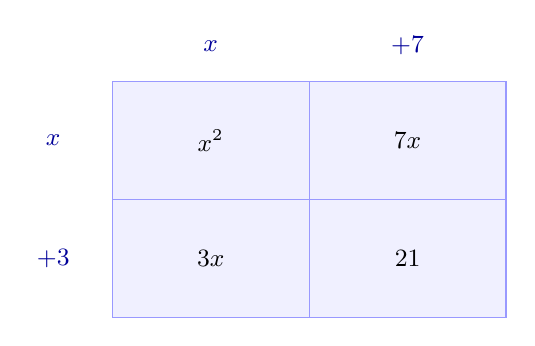
\begin{tikzpicture}[font=\small]
  \fill[blue!6] (0,0) rectangle (2.5,-1.5);
  \draw[blue!40] (0,0) rectangle (2.5,-1.5);
  \node at (1.25,-0.75) {$x^{2}$};
  \fill[blue!6] (2.5,0) rectangle (5,-1.5);
  \draw[blue!40] (2.5,0) rectangle (5,-1.5);
  \node at (3.75,-0.75) {$7x$};
  \fill[blue!6] (0,-1.5) rectangle (2.5,-3);
  \draw[blue!40] (0,-1.5) rectangle (2.5,-3);
  \node at (1.25,-2.25) {$3x$};
  \fill[blue!6] (2.5,-1.5) rectangle (5,-3);
  \draw[blue!40] (2.5,-1.5) rectangle (5,-3);
  \node at (3.75,-2.25) {$21$};
  \node[blue!60!black] at (1.25,0.45) {$x$};
  \node[blue!60!black] at (3.75,0.45) {$+7$};
  \node[blue!60!black] at (-0.75,-0.75) {$x$};
  \node[blue!60!black] at (-0.75,-2.25) {$+3$};
\end{tikzpicture} &
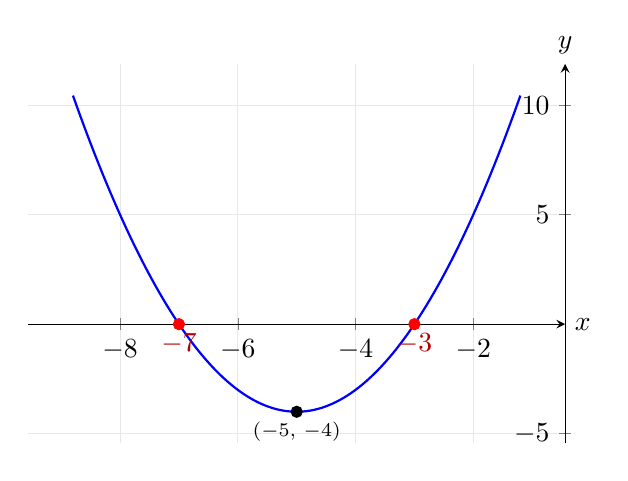
\begin{tikzpicture}
\begin{axis}[
  axis lines=middle, xlabel={$x$}, ylabel={$y$},
  width=8.4cm, height=6.4cm, grid=both, grid style={gray!18},
  enlargelimits=true, samples=120,
  domain=-8.8:-1.2, every axis x label/.style={at={(ticklabel* cs:1)},anchor=west},
  every axis y label/.style={at={(ticklabel* cs:1)},anchor=south}]
  \addplot[blue, thick]{1*x^2 + 10*x + 21};
  \addplot[only marks, mark=*, red] coordinates {(-3,0)};
  \node[red!70!black, anchor=north] at (axis cs:-3,0) {$-3$};
  \addplot[only marks, mark=*, red] coordinates {(-7,0)};
  \node[red!70!black, anchor=north] at (axis cs:-7,0) {$-7$};
  \addplot[only marks, mark=*, black] coordinates {(-5,-4)};
  \node[anchor=north] at (axis cs:-5,-4) {\scriptsize $(-5,\,-4)$};
\end{axis}
\end{tikzpicture}
\\[4pt]
{\small (a) Area / box model} & {\small (b) Graph $y=f(x)$ with its roots} \\
\end{tabular}
\end{center}
\vspace{2pt}\hrule\vspace{6pt}

\section*{Question 6 \quad {\normalfont\small\ttfamily qc1-006}}
\addcontentsline{toc}{section}{Q6. Monic ($a=1$)}
\nopagebreak
\begin{qbox}
Factorise: \( x^2 - 7x + 10 \)
\end{qbox}
\smallskip\noindent\textit{Type:} Monic ($a=1$) \hfill \textit{Marks:} 2 \quad \textit{Difficulty:} Foundation\\[2pt]
\subsection*{Worked solution}
\begin{enumerate}[leftmargin=1.6em,label=\textbf{Step \arabic*.}]
  \item Set up brackets.
  \[ (x \quad )(x \quad ) \]
  \par\smallskip{\small\itshape Monic quadratic.}
  \item Find two numbers that multiply to 10 and add to \( -7 \).
  \[ (-2) \times (-5) = 10, \quad (-2) + (-5) = -7 \]
  \par\smallskip{\small\itshape c is positive and b is negative, so both signs are negative.}
  \item Write the factorised form.
  \[ (x - 2)(x - 5) \]
  \par\smallskip{\small\itshape Both factors negative.}
\end{enumerate}
\begin{ansbox}\textbf{Final answer:}\quad \((x - 2)(x - 5)\)\end{ansbox}
\subsection*{Check by expanding}
Multiplying the brackets back out reproduces the original expression:
\[ x^{2} -5x -2x +10 \]
\subsection*{Visualising the factorisation}
\begin{center}
\begin{tabular}{cc}
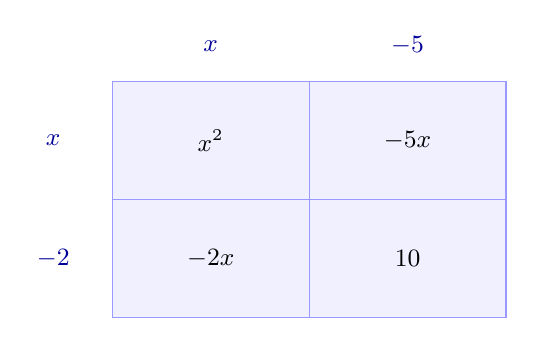
\begin{tikzpicture}[font=\small]
  \fill[blue!6] (0,0) rectangle (2.5,-1.5);
  \draw[blue!40] (0,0) rectangle (2.5,-1.5);
  \node at (1.25,-0.75) {$x^{2}$};
  \fill[blue!6] (2.5,0) rectangle (5,-1.5);
  \draw[blue!40] (2.5,0) rectangle (5,-1.5);
  \node at (3.75,-0.75) {$-5x$};
  \fill[blue!6] (0,-1.5) rectangle (2.5,-3);
  \draw[blue!40] (0,-1.5) rectangle (2.5,-3);
  \node at (1.25,-2.25) {$-2x$};
  \fill[blue!6] (2.5,-1.5) rectangle (5,-3);
  \draw[blue!40] (2.5,-1.5) rectangle (5,-3);
  \node at (3.75,-2.25) {$10$};
  \node[blue!60!black] at (1.25,0.45) {$x$};
  \node[blue!60!black] at (3.75,0.45) {$-5$};
  \node[blue!60!black] at (-0.75,-0.75) {$x$};
  \node[blue!60!black] at (-0.75,-2.25) {$-2$};
\end{tikzpicture} &
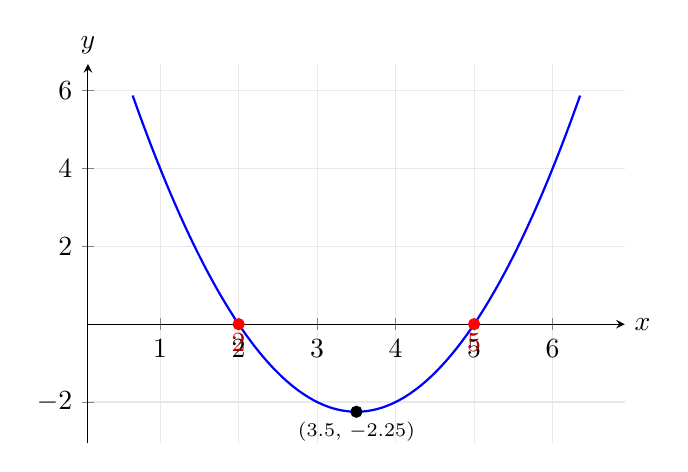
\begin{tikzpicture}
\begin{axis}[
  axis lines=middle, xlabel={$x$}, ylabel={$y$},
  width=8.4cm, height=6.4cm, grid=both, grid style={gray!18},
  enlargelimits=true, samples=120,
  domain=0.65:6.35, every axis x label/.style={at={(ticklabel* cs:1)},anchor=west},
  every axis y label/.style={at={(ticklabel* cs:1)},anchor=south}]
  \addplot[blue, thick]{1*x^2 - 7*x + 10};
  \addplot[only marks, mark=*, red] coordinates {(2,0)};
  \node[red!70!black, anchor=north] at (axis cs:2,0) {$2$};
  \addplot[only marks, mark=*, red] coordinates {(5,0)};
  \node[red!70!black, anchor=north] at (axis cs:5,0) {$5$};
  \addplot[only marks, mark=*, black] coordinates {(3.5,-2.25)};
  \node[anchor=north] at (axis cs:3.5,-2.25) {\scriptsize $(3.5,\,-2.25)$};
\end{axis}
\end{tikzpicture}
\\[4pt]
{\small (a) Area / box model} & {\small (b) Graph $y=f(x)$ with its roots} \\
\end{tabular}
\end{center}
\vspace{2pt}\hrule\vspace{6pt}

\section*{Question 7 \quad {\normalfont\small\ttfamily qc1-007}}
\addcontentsline{toc}{section}{Q7. Monic ($a=1$)}
\nopagebreak
\begin{qbox}
Factorise: \( x^2 - 9x + 18 \)
\end{qbox}
\smallskip\noindent\textit{Type:} Monic ($a=1$) \hfill \textit{Marks:} 2 \quad \textit{Difficulty:} Foundation\\[2pt]
\subsection*{Worked solution}
\begin{enumerate}[leftmargin=1.6em,label=\textbf{Step \arabic*.}]
  \item Set up brackets.
  \[ (x \quad )(x \quad ) \]
  \par\smallskip{\small\itshape Monic quadratic.}
  \item Find numbers multiplying to 18 and adding to \( -9 \).
  \[ (-3) \times (-6) = 18, \quad (-3) + (-6) = -9 \]
  \par\smallskip{\small\itshape Both signs negative because c > 0 and b < 0.}
  \item Write the answer.
  \[ (x - 3)(x - 6) \]
  \par\smallskip{\small\itshape Both factors are negative.}
\end{enumerate}
\begin{ansbox}\textbf{Final answer:}\quad \((x - 3)(x - 6)\)\end{ansbox}
\subsection*{Check by expanding}
Multiplying the brackets back out reproduces the original expression:
\[ x^{2} -6x -3x +18 \]
\subsection*{Visualising the factorisation}
\begin{center}
\begin{tabular}{cc}
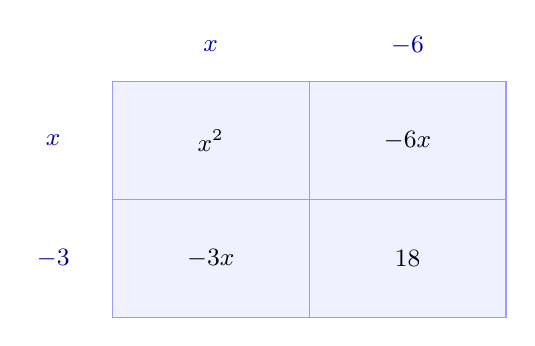
\begin{tikzpicture}[font=\small]
  \fill[blue!6] (0,0) rectangle (2.5,-1.5);
  \draw[blue!40] (0,0) rectangle (2.5,-1.5);
  \node at (1.25,-0.75) {$x^{2}$};
  \fill[blue!6] (2.5,0) rectangle (5,-1.5);
  \draw[blue!40] (2.5,0) rectangle (5,-1.5);
  \node at (3.75,-0.75) {$-6x$};
  \fill[blue!6] (0,-1.5) rectangle (2.5,-3);
  \draw[blue!40] (0,-1.5) rectangle (2.5,-3);
  \node at (1.25,-2.25) {$-3x$};
  \fill[blue!6] (2.5,-1.5) rectangle (5,-3);
  \draw[blue!40] (2.5,-1.5) rectangle (5,-3);
  \node at (3.75,-2.25) {$18$};
  \node[blue!60!black] at (1.25,0.45) {$x$};
  \node[blue!60!black] at (3.75,0.45) {$-6$};
  \node[blue!60!black] at (-0.75,-0.75) {$x$};
  \node[blue!60!black] at (-0.75,-2.25) {$-3$};
\end{tikzpicture} &
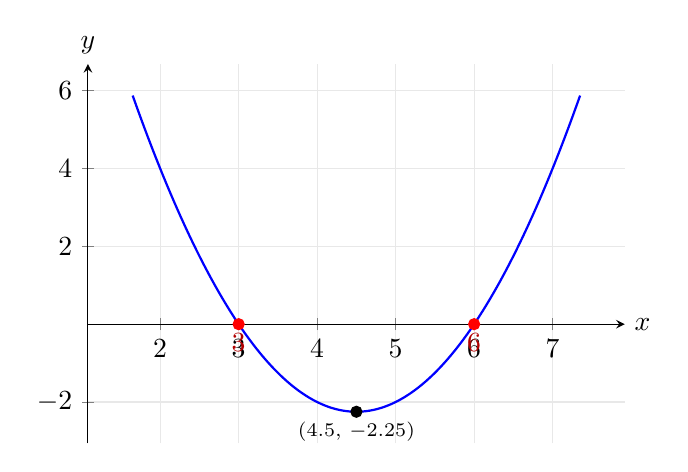
\begin{tikzpicture}
\begin{axis}[
  axis lines=middle, xlabel={$x$}, ylabel={$y$},
  width=8.4cm, height=6.4cm, grid=both, grid style={gray!18},
  enlargelimits=true, samples=120,
  domain=1.65:7.35, every axis x label/.style={at={(ticklabel* cs:1)},anchor=west},
  every axis y label/.style={at={(ticklabel* cs:1)},anchor=south}]
  \addplot[blue, thick]{1*x^2 - 9*x + 18};
  \addplot[only marks, mark=*, red] coordinates {(3,0)};
  \node[red!70!black, anchor=north] at (axis cs:3,0) {$3$};
  \addplot[only marks, mark=*, red] coordinates {(6,0)};
  \node[red!70!black, anchor=north] at (axis cs:6,0) {$6$};
  \addplot[only marks, mark=*, black] coordinates {(4.5,-2.25)};
  \node[anchor=north] at (axis cs:4.5,-2.25) {\scriptsize $(4.5,\,-2.25)$};
\end{axis}
\end{tikzpicture}
\\[4pt]
{\small (a) Area / box model} & {\small (b) Graph $y=f(x)$ with its roots} \\
\end{tabular}
\end{center}
\vspace{2pt}\hrule\vspace{6pt}

\section*{Question 8 \quad {\normalfont\small\ttfamily qc1-008}}
\addcontentsline{toc}{section}{Q8. Monic ($a=1$)}
\nopagebreak
\begin{qbox}
Factorise: \( x^2 - 11x + 28 \)
\end{qbox}
\smallskip\noindent\textit{Type:} Monic ($a=1$) \hfill \textit{Marks:} 2 \quad \textit{Difficulty:} Foundation\\[2pt]
\subsection*{Worked solution}
\begin{enumerate}[leftmargin=1.6em,label=\textbf{Step \arabic*.}]
  \item Set up brackets.
  \[ (x \quad )(x \quad ) \]
  \par\smallskip{\small\itshape Leading coefficient is 1.}
  \item Find numbers multiplying to 28 and adding to \( -11 \).
  \[ (-4) \times (-7) = 28, \quad (-4) + (-7) = -11 \]
  \par\smallskip{\small\itshape Both signs negative.}
  \item Write the answer.
  \[ (x - 4)(x - 7) \]
  \par\smallskip{\small\itshape Both factors are negative.}
\end{enumerate}
\begin{ansbox}\textbf{Final answer:}\quad \((x - 4)(x - 7)\)\end{ansbox}
\subsection*{Check by expanding}
Multiplying the brackets back out reproduces the original expression:
\[ x^{2} -7x -4x +28 \]
\subsection*{Visualising the factorisation}
\begin{center}
\begin{tabular}{cc}
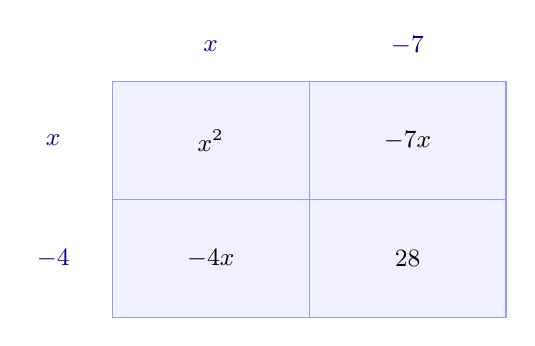
\begin{tikzpicture}[font=\small]
  \fill[blue!6] (0,0) rectangle (2.5,-1.5);
  \draw[blue!40] (0,0) rectangle (2.5,-1.5);
  \node at (1.25,-0.75) {$x^{2}$};
  \fill[blue!6] (2.5,0) rectangle (5,-1.5);
  \draw[blue!40] (2.5,0) rectangle (5,-1.5);
  \node at (3.75,-0.75) {$-7x$};
  \fill[blue!6] (0,-1.5) rectangle (2.5,-3);
  \draw[blue!40] (0,-1.5) rectangle (2.5,-3);
  \node at (1.25,-2.25) {$-4x$};
  \fill[blue!6] (2.5,-1.5) rectangle (5,-3);
  \draw[blue!40] (2.5,-1.5) rectangle (5,-3);
  \node at (3.75,-2.25) {$28$};
  \node[blue!60!black] at (1.25,0.45) {$x$};
  \node[blue!60!black] at (3.75,0.45) {$-7$};
  \node[blue!60!black] at (-0.75,-0.75) {$x$};
  \node[blue!60!black] at (-0.75,-2.25) {$-4$};
\end{tikzpicture} &
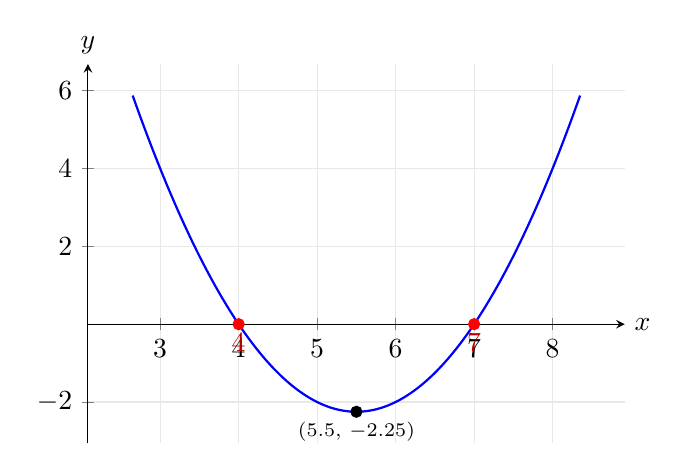
\begin{tikzpicture}
\begin{axis}[
  axis lines=middle, xlabel={$x$}, ylabel={$y$},
  width=8.4cm, height=6.4cm, grid=both, grid style={gray!18},
  enlargelimits=true, samples=120,
  domain=2.65:8.35, every axis x label/.style={at={(ticklabel* cs:1)},anchor=west},
  every axis y label/.style={at={(ticklabel* cs:1)},anchor=south}]
  \addplot[blue, thick]{1*x^2 - 11*x + 28};
  \addplot[only marks, mark=*, red] coordinates {(4,0)};
  \node[red!70!black, anchor=north] at (axis cs:4,0) {$4$};
  \addplot[only marks, mark=*, red] coordinates {(7,0)};
  \node[red!70!black, anchor=north] at (axis cs:7,0) {$7$};
  \addplot[only marks, mark=*, black] coordinates {(5.5,-2.25)};
  \node[anchor=north] at (axis cs:5.5,-2.25) {\scriptsize $(5.5,\,-2.25)$};
\end{axis}
\end{tikzpicture}
\\[4pt]
{\small (a) Area / box model} & {\small (b) Graph $y=f(x)$ with its roots} \\
\end{tabular}
\end{center}
\vspace{2pt}\hrule\vspace{6pt}

\section*{Question 9 \quad {\normalfont\small\ttfamily qc1-009}}
\addcontentsline{toc}{section}{Q9. Monic ($a=1$)}
\nopagebreak
\begin{qbox}
Factorise: \( x^2 - 13x + 36 \)
\end{qbox}
\smallskip\noindent\textit{Type:} Monic ($a=1$) \hfill \textit{Marks:} 2 \quad \textit{Difficulty:} Foundation\\[2pt]
\subsection*{Worked solution}
\begin{enumerate}[leftmargin=1.6em,label=\textbf{Step \arabic*.}]
  \item Set up brackets.
  \[ (x \quad )(x \quad ) \]
  \par\smallskip{\small\itshape Monic quadratic.}
  \item Find numbers multiplying to 36 and adding to \( -13 \).
  \[ (-4) \times (-9) = 36, \quad (-4) + (-9) = -13 \]
  \par\smallskip{\small\itshape Factor pairs of 36: (1,36),(2,18),(3,12),(4,9),(6,6). The pair (4,9) adds to 13.}
  \item Write the answer.
  \[ (x - 4)(x - 9) \]
  \par\smallskip{\small\itshape Both signs negative.}
\end{enumerate}
\begin{ansbox}\textbf{Final answer:}\quad \((x - 4)(x - 9)\)\end{ansbox}
\subsection*{Check by expanding}
Multiplying the brackets back out reproduces the original expression:
\[ x^{2} -9x -4x +36 \]
\subsection*{Visualising the factorisation}
\begin{center}
\begin{tabular}{cc}
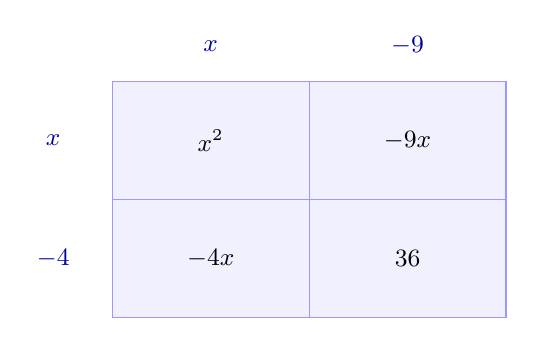
\begin{tikzpicture}[font=\small]
  \fill[blue!6] (0,0) rectangle (2.5,-1.5);
  \draw[blue!40] (0,0) rectangle (2.5,-1.5);
  \node at (1.25,-0.75) {$x^{2}$};
  \fill[blue!6] (2.5,0) rectangle (5,-1.5);
  \draw[blue!40] (2.5,0) rectangle (5,-1.5);
  \node at (3.75,-0.75) {$-9x$};
  \fill[blue!6] (0,-1.5) rectangle (2.5,-3);
  \draw[blue!40] (0,-1.5) rectangle (2.5,-3);
  \node at (1.25,-2.25) {$-4x$};
  \fill[blue!6] (2.5,-1.5) rectangle (5,-3);
  \draw[blue!40] (2.5,-1.5) rectangle (5,-3);
  \node at (3.75,-2.25) {$36$};
  \node[blue!60!black] at (1.25,0.45) {$x$};
  \node[blue!60!black] at (3.75,0.45) {$-9$};
  \node[blue!60!black] at (-0.75,-0.75) {$x$};
  \node[blue!60!black] at (-0.75,-2.25) {$-4$};
\end{tikzpicture} &
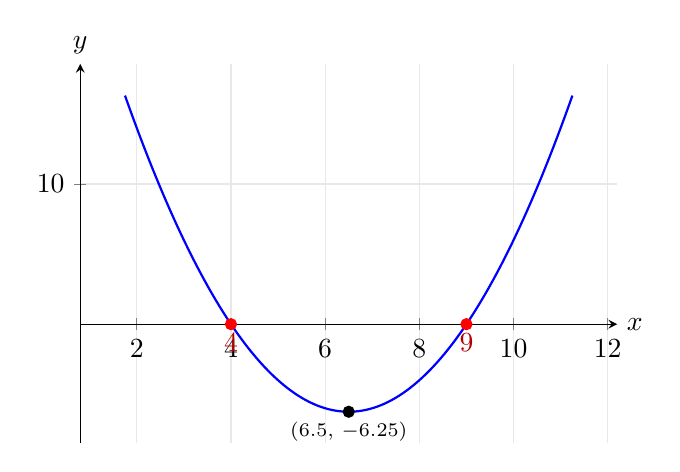
\begin{tikzpicture}
\begin{axis}[
  axis lines=middle, xlabel={$x$}, ylabel={$y$},
  width=8.4cm, height=6.4cm, grid=both, grid style={gray!18},
  enlargelimits=true, samples=120,
  domain=1.75:11.25, every axis x label/.style={at={(ticklabel* cs:1)},anchor=west},
  every axis y label/.style={at={(ticklabel* cs:1)},anchor=south}]
  \addplot[blue, thick]{1*x^2 - 13*x + 36};
  \addplot[only marks, mark=*, red] coordinates {(4,0)};
  \node[red!70!black, anchor=north] at (axis cs:4,0) {$4$};
  \addplot[only marks, mark=*, red] coordinates {(9,0)};
  \node[red!70!black, anchor=north] at (axis cs:9,0) {$9$};
  \addplot[only marks, mark=*, black] coordinates {(6.5,-6.25)};
  \node[anchor=north] at (axis cs:6.5,-6.25) {\scriptsize $(6.5,\,-6.25)$};
\end{axis}
\end{tikzpicture}
\\[4pt]
{\small (a) Area / box model} & {\small (b) Graph $y=f(x)$ with its roots} \\
\end{tabular}
\end{center}
\vspace{2pt}\hrule\vspace{6pt}

\section*{Question 10 \quad {\normalfont\small\ttfamily qc1-010}}
\addcontentsline{toc}{section}{Q10. Monic ($a=1$)}
\nopagebreak
\begin{qbox}
Factorise: \( x^2 - 15x + 56 \)
\end{qbox}
\smallskip\noindent\textit{Type:} Monic ($a=1$) \hfill \textit{Marks:} 2 \quad \textit{Difficulty:} Foundation\\[2pt]
\subsection*{Worked solution}
\begin{enumerate}[leftmargin=1.6em,label=\textbf{Step \arabic*.}]
  \item Set up brackets.
  \[ (x \quad )(x \quad ) \]
  \par\smallskip{\small\itshape Monic quadratic.}
  \item Find numbers multiplying to 56 and adding to \( -15 \).
  \[ (-7) \times (-8) = 56, \quad (-7) + (-8) = -15 \]
  \par\smallskip{\small\itshape Factor pairs: (1,56),(2,28),(4,14),(7,8). (7,8) adds to 15.}
  \item Write the answer.
  \[ (x - 7)(x - 8) \]
  \par\smallskip{\small\itshape Both signs negative.}
\end{enumerate}
\begin{ansbox}\textbf{Final answer:}\quad \((x - 7)(x - 8)\)\end{ansbox}
\subsection*{Check by expanding}
Multiplying the brackets back out reproduces the original expression:
\[ x^{2} -8x -7x +56 \]
\subsection*{Visualising the factorisation}
\begin{center}
\begin{tabular}{cc}
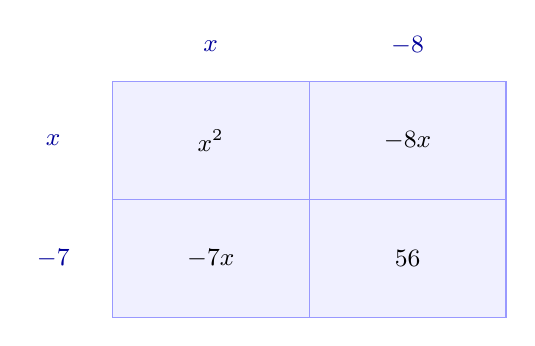
\begin{tikzpicture}[font=\small]
  \fill[blue!6] (0,0) rectangle (2.5,-1.5);
  \draw[blue!40] (0,0) rectangle (2.5,-1.5);
  \node at (1.25,-0.75) {$x^{2}$};
  \fill[blue!6] (2.5,0) rectangle (5,-1.5);
  \draw[blue!40] (2.5,0) rectangle (5,-1.5);
  \node at (3.75,-0.75) {$-8x$};
  \fill[blue!6] (0,-1.5) rectangle (2.5,-3);
  \draw[blue!40] (0,-1.5) rectangle (2.5,-3);
  \node at (1.25,-2.25) {$-7x$};
  \fill[blue!6] (2.5,-1.5) rectangle (5,-3);
  \draw[blue!40] (2.5,-1.5) rectangle (5,-3);
  \node at (3.75,-2.25) {$56$};
  \node[blue!60!black] at (1.25,0.45) {$x$};
  \node[blue!60!black] at (3.75,0.45) {$-8$};
  \node[blue!60!black] at (-0.75,-0.75) {$x$};
  \node[blue!60!black] at (-0.75,-2.25) {$-7$};
\end{tikzpicture} &
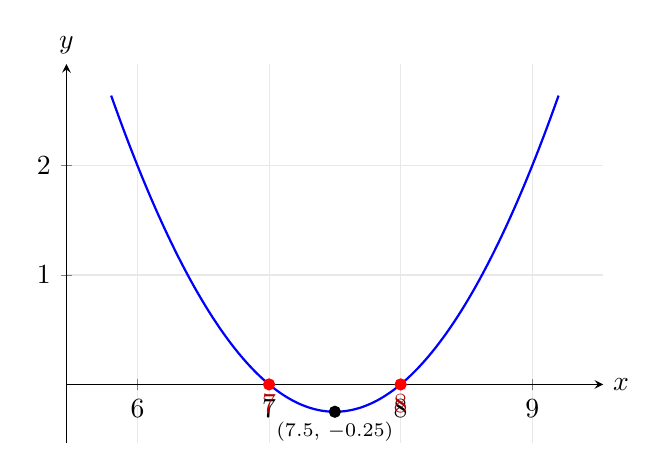
\begin{tikzpicture}
\begin{axis}[
  axis lines=middle, xlabel={$x$}, ylabel={$y$},
  width=8.4cm, height=6.4cm, grid=both, grid style={gray!18},
  enlargelimits=true, samples=120,
  domain=5.8:9.2, every axis x label/.style={at={(ticklabel* cs:1)},anchor=west},
  every axis y label/.style={at={(ticklabel* cs:1)},anchor=south}]
  \addplot[blue, thick]{1*x^2 - 15*x + 56};
  \addplot[only marks, mark=*, red] coordinates {(7,0)};
  \node[red!70!black, anchor=north] at (axis cs:7,0) {$7$};
  \addplot[only marks, mark=*, red] coordinates {(8,0)};
  \node[red!70!black, anchor=north] at (axis cs:8,0) {$8$};
  \addplot[only marks, mark=*, black] coordinates {(7.5,-0.25)};
  \node[anchor=north] at (axis cs:7.5,-0.25) {\scriptsize $(7.5,\,-0.25)$};
\end{axis}
\end{tikzpicture}
\\[4pt]
{\small (a) Area / box model} & {\small (b) Graph $y=f(x)$ with its roots} \\
\end{tabular}
\end{center}
\vspace{2pt}\hrule\vspace{6pt}

\section*{Question 11 \quad {\normalfont\small\ttfamily qc1-011}}
\addcontentsline{toc}{section}{Q11. Monic ($a=1$)}
\nopagebreak
\begin{qbox}
Factorise: \( x^2 + 2x - 15 \)
\end{qbox}
\smallskip\noindent\textit{Type:} Monic ($a=1$) \hfill \textit{Marks:} 2 \quad \textit{Difficulty:} Foundation\\[2pt]
\subsection*{Worked solution}
\begin{enumerate}[leftmargin=1.6em,label=\textbf{Step \arabic*.}]
  \item Set up brackets.
  \[ (x \quad )(x \quad ) \]
  \par\smallskip{\small\itshape Monic quadratic.}
  \item Find numbers multiplying to \( -15 \) and adding to \( +2 \).
  \[ 5 \times (-3) = -15, \quad 5 + (-3) = 2 \]
  \par\smallskip{\small\itshape c is negative so the signs are opposite.}
  \item Write the answer.
  \[ (x + 5)(x - 3) \]
  \par\smallskip{\small\itshape The larger number (5) takes the positive sign.}
\end{enumerate}
\begin{ansbox}\textbf{Final answer:}\quad \((x + 5)(x - 3)\)\end{ansbox}
\subsection*{Check by expanding}
Multiplying the brackets back out reproduces the original expression:
\[ x^{2} -3x +5x -15 \]
\subsection*{Visualising the factorisation}
\begin{center}
\begin{tabular}{cc}
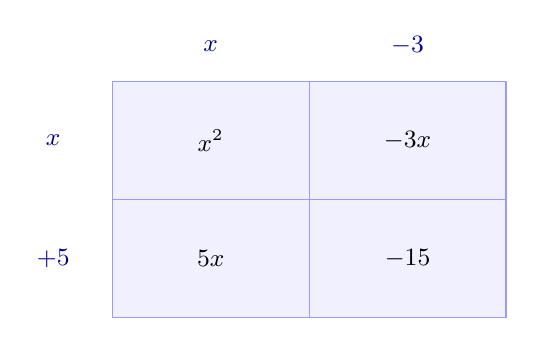
\begin{tikzpicture}[font=\small]
  \fill[blue!6] (0,0) rectangle (2.5,-1.5);
  \draw[blue!40] (0,0) rectangle (2.5,-1.5);
  \node at (1.25,-0.75) {$x^{2}$};
  \fill[blue!6] (2.5,0) rectangle (5,-1.5);
  \draw[blue!40] (2.5,0) rectangle (5,-1.5);
  \node at (3.75,-0.75) {$-3x$};
  \fill[blue!6] (0,-1.5) rectangle (2.5,-3);
  \draw[blue!40] (0,-1.5) rectangle (2.5,-3);
  \node at (1.25,-2.25) {$5x$};
  \fill[blue!6] (2.5,-1.5) rectangle (5,-3);
  \draw[blue!40] (2.5,-1.5) rectangle (5,-3);
  \node at (3.75,-2.25) {$-15$};
  \node[blue!60!black] at (1.25,0.45) {$x$};
  \node[blue!60!black] at (3.75,0.45) {$-3$};
  \node[blue!60!black] at (-0.75,-0.75) {$x$};
  \node[blue!60!black] at (-0.75,-2.25) {$+5$};
\end{tikzpicture} &
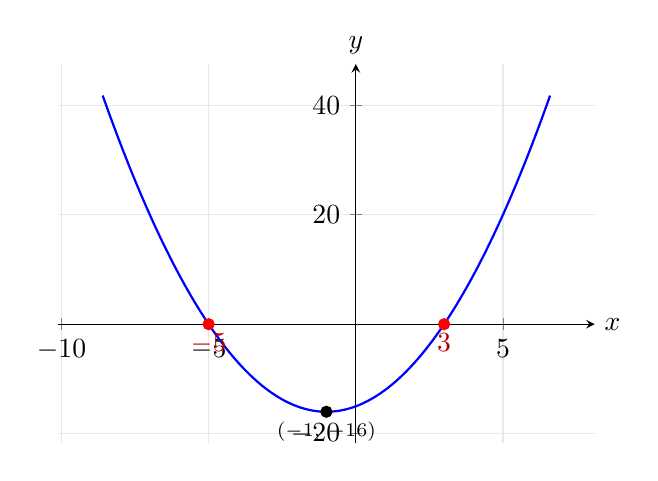
\begin{tikzpicture}
\begin{axis}[
  axis lines=middle, xlabel={$x$}, ylabel={$y$},
  width=8.4cm, height=6.4cm, grid=both, grid style={gray!18},
  enlargelimits=true, samples=120,
  domain=-8.6:6.6, every axis x label/.style={at={(ticklabel* cs:1)},anchor=west},
  every axis y label/.style={at={(ticklabel* cs:1)},anchor=south}]
  \addplot[blue, thick]{1*x^2 + 2*x - 15};
  \addplot[only marks, mark=*, red] coordinates {(-5,0)};
  \node[red!70!black, anchor=north] at (axis cs:-5,0) {$-5$};
  \addplot[only marks, mark=*, red] coordinates {(3,0)};
  \node[red!70!black, anchor=north] at (axis cs:3,0) {$3$};
  \addplot[only marks, mark=*, black] coordinates {(-1,-16)};
  \node[anchor=north] at (axis cs:-1,-16) {\scriptsize $(-1,\,-16)$};
\end{axis}
\end{tikzpicture}
\\[4pt]
{\small (a) Area / box model} & {\small (b) Graph $y=f(x)$ with its roots} \\
\end{tabular}
\end{center}
\vspace{2pt}\hrule\vspace{6pt}

\section*{Question 12 \quad {\normalfont\small\ttfamily qc1-012}}
\addcontentsline{toc}{section}{Q12. Monic ($a=1$)}
\nopagebreak
\begin{qbox}
Factorise: \( x^2 + 4x - 21 \)
\end{qbox}
\smallskip\noindent\textit{Type:} Monic ($a=1$) \hfill \textit{Marks:} 2 \quad \textit{Difficulty:} Foundation\\[2pt]
\subsection*{Worked solution}
\begin{enumerate}[leftmargin=1.6em,label=\textbf{Step \arabic*.}]
  \item Set up brackets.
  \[ (x \quad )(x \quad ) \]
  \par\smallskip{\small\itshape Monic quadratic.}
  \item Find numbers multiplying to \( -21 \) and adding to \( +4 \).
  \[ 7 \times (-3) = -21, \quad 7 + (-3) = 4 \]
  \par\smallskip{\small\itshape Opposite signs because c is negative.}
  \item Write the answer.
  \[ (x + 7)(x - 3) \]
  \par\smallskip{\small\itshape The larger value 7 is positive.}
\end{enumerate}
\begin{ansbox}\textbf{Final answer:}\quad \((x + 7)(x - 3)\)\end{ansbox}
\subsection*{Check by expanding}
Multiplying the brackets back out reproduces the original expression:
\[ x^{2} -3x +7x -21 \]
\subsection*{Visualising the factorisation}
\begin{center}
\begin{tabular}{cc}
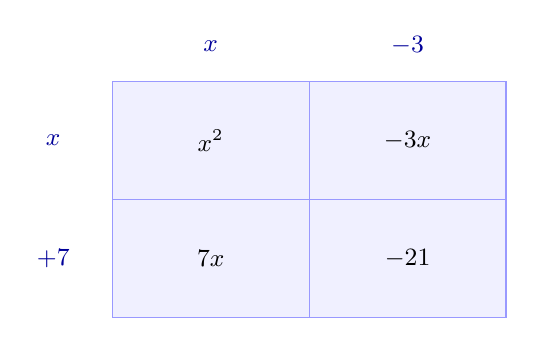
\begin{tikzpicture}[font=\small]
  \fill[blue!6] (0,0) rectangle (2.5,-1.5);
  \draw[blue!40] (0,0) rectangle (2.5,-1.5);
  \node at (1.25,-0.75) {$x^{2}$};
  \fill[blue!6] (2.5,0) rectangle (5,-1.5);
  \draw[blue!40] (2.5,0) rectangle (5,-1.5);
  \node at (3.75,-0.75) {$-3x$};
  \fill[blue!6] (0,-1.5) rectangle (2.5,-3);
  \draw[blue!40] (0,-1.5) rectangle (2.5,-3);
  \node at (1.25,-2.25) {$7x$};
  \fill[blue!6] (2.5,-1.5) rectangle (5,-3);
  \draw[blue!40] (2.5,-1.5) rectangle (5,-3);
  \node at (3.75,-2.25) {$-21$};
  \node[blue!60!black] at (1.25,0.45) {$x$};
  \node[blue!60!black] at (3.75,0.45) {$-3$};
  \node[blue!60!black] at (-0.75,-0.75) {$x$};
  \node[blue!60!black] at (-0.75,-2.25) {$+7$};
\end{tikzpicture} &
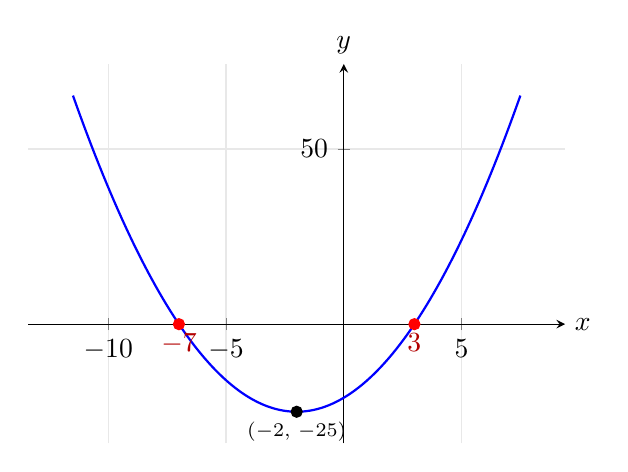
\begin{tikzpicture}
\begin{axis}[
  axis lines=middle, xlabel={$x$}, ylabel={$y$},
  width=8.4cm, height=6.4cm, grid=both, grid style={gray!18},
  enlargelimits=true, samples=120,
  domain=-11.5:7.5, every axis x label/.style={at={(ticklabel* cs:1)},anchor=west},
  every axis y label/.style={at={(ticklabel* cs:1)},anchor=south}]
  \addplot[blue, thick]{1*x^2 + 4*x - 21};
  \addplot[only marks, mark=*, red] coordinates {(-7,0)};
  \node[red!70!black, anchor=north] at (axis cs:-7,0) {$-7$};
  \addplot[only marks, mark=*, red] coordinates {(3,0)};
  \node[red!70!black, anchor=north] at (axis cs:3,0) {$3$};
  \addplot[only marks, mark=*, black] coordinates {(-2,-25)};
  \node[anchor=north] at (axis cs:-2,-25) {\scriptsize $(-2,\,-25)$};
\end{axis}
\end{tikzpicture}
\\[4pt]
{\small (a) Area / box model} & {\small (b) Graph $y=f(x)$ with its roots} \\
\end{tabular}
\end{center}
\vspace{2pt}\hrule\vspace{6pt}

\section*{Question 13 \quad {\normalfont\small\ttfamily qc1-013}}
\addcontentsline{toc}{section}{Q13. Monic ($a=1$)}
\nopagebreak
\begin{qbox}
Factorise: \( x^2 + 3x - 28 \)
\end{qbox}
\smallskip\noindent\textit{Type:} Monic ($a=1$) \hfill \textit{Marks:} 2 \quad \textit{Difficulty:} Foundation\\[2pt]
\subsection*{Worked solution}
\begin{enumerate}[leftmargin=1.6em,label=\textbf{Step \arabic*.}]
  \item Set up brackets.
  \[ (x \quad )(x \quad ) \]
  \par\smallskip{\small\itshape Monic quadratic.}
  \item Find numbers multiplying to \( -28 \) and adding to \( +3 \).
  \[ 7 \times (-4) = -28, \quad 7 + (-4) = 3 \]
  \par\smallskip{\small\itshape Factor pairs of 28: (1,28),(2,14),(4,7). (4,7) gives a difference of 3.}
  \item Write the answer.
  \[ (x + 7)(x - 4) \]
  \par\smallskip{\small\itshape Larger number (7) is positive.}
\end{enumerate}
\begin{ansbox}\textbf{Final answer:}\quad \((x + 7)(x - 4)\)\end{ansbox}
\subsection*{Check by expanding}
Multiplying the brackets back out reproduces the original expression:
\[ x^{2} -4x +7x -28 \]
\subsection*{Visualising the factorisation}
\begin{center}
\begin{tabular}{cc}
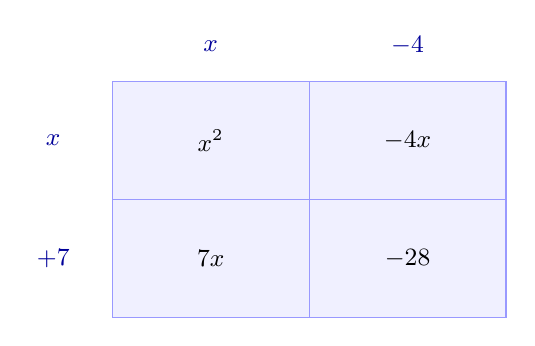
\begin{tikzpicture}[font=\small]
  \fill[blue!6] (0,0) rectangle (2.5,-1.5);
  \draw[blue!40] (0,0) rectangle (2.5,-1.5);
  \node at (1.25,-0.75) {$x^{2}$};
  \fill[blue!6] (2.5,0) rectangle (5,-1.5);
  \draw[blue!40] (2.5,0) rectangle (5,-1.5);
  \node at (3.75,-0.75) {$-4x$};
  \fill[blue!6] (0,-1.5) rectangle (2.5,-3);
  \draw[blue!40] (0,-1.5) rectangle (2.5,-3);
  \node at (1.25,-2.25) {$7x$};
  \fill[blue!6] (2.5,-1.5) rectangle (5,-3);
  \draw[blue!40] (2.5,-1.5) rectangle (5,-3);
  \node at (3.75,-2.25) {$-28$};
  \node[blue!60!black] at (1.25,0.45) {$x$};
  \node[blue!60!black] at (3.75,0.45) {$-4$};
  \node[blue!60!black] at (-0.75,-0.75) {$x$};
  \node[blue!60!black] at (-0.75,-2.25) {$+7$};
\end{tikzpicture} &
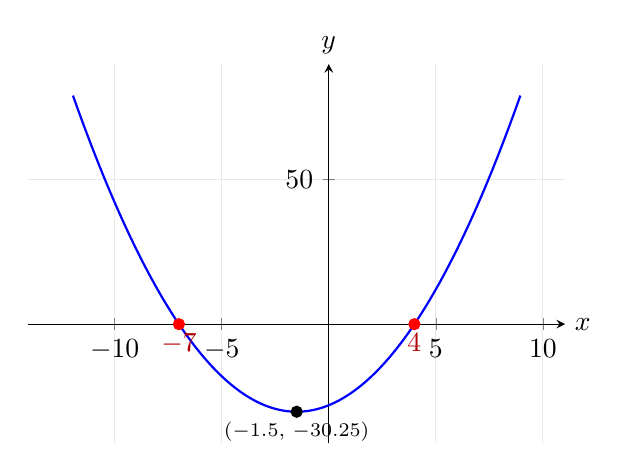
\begin{tikzpicture}
\begin{axis}[
  axis lines=middle, xlabel={$x$}, ylabel={$y$},
  width=8.4cm, height=6.4cm, grid=both, grid style={gray!18},
  enlargelimits=true, samples=120,
  domain=-11.95:8.95, every axis x label/.style={at={(ticklabel* cs:1)},anchor=west},
  every axis y label/.style={at={(ticklabel* cs:1)},anchor=south}]
  \addplot[blue, thick]{1*x^2 + 3*x - 28};
  \addplot[only marks, mark=*, red] coordinates {(-7,0)};
  \node[red!70!black, anchor=north] at (axis cs:-7,0) {$-7$};
  \addplot[only marks, mark=*, red] coordinates {(4,0)};
  \node[red!70!black, anchor=north] at (axis cs:4,0) {$4$};
  \addplot[only marks, mark=*, black] coordinates {(-1.5,-30.25)};
  \node[anchor=north] at (axis cs:-1.5,-30.25) {\scriptsize $(-1.5,\,-30.25)$};
\end{axis}
\end{tikzpicture}
\\[4pt]
{\small (a) Area / box model} & {\small (b) Graph $y=f(x)$ with its roots} \\
\end{tabular}
\end{center}
\vspace{2pt}\hrule\vspace{6pt}

\section*{Question 14 \quad {\normalfont\small\ttfamily qc1-014}}
\addcontentsline{toc}{section}{Q14. Monic ($a=1$)}
\nopagebreak
\begin{qbox}
Factorise: \( x^2 + 5x - 24 \)
\end{qbox}
\smallskip\noindent\textit{Type:} Monic ($a=1$) \hfill \textit{Marks:} 2 \quad \textit{Difficulty:} Foundation\\[2pt]
\subsection*{Worked solution}
\begin{enumerate}[leftmargin=1.6em,label=\textbf{Step \arabic*.}]
  \item Set up brackets.
  \[ (x \quad )(x \quad ) \]
  \par\smallskip{\small\itshape Monic quadratic.}
  \item Find numbers multiplying to \( -24 \) and adding to \( +5 \).
  \[ 8 \times (-3) = -24, \quad 8 + (-3) = 5 \]
  \par\smallskip{\small\itshape Factor pairs of 24: (1,24),(2,12),(3,8),(4,6). (3,8) gives a difference of 5.}
  \item Write the answer.
  \[ (x + 8)(x - 3) \]
  \par\smallskip{\small\itshape Larger (8) is positive.}
\end{enumerate}
\begin{ansbox}\textbf{Final answer:}\quad \((x + 8)(x - 3)\)\end{ansbox}
\subsection*{Check by expanding}
Multiplying the brackets back out reproduces the original expression:
\[ x^{2} -3x +8x -24 \]
\subsection*{Visualising the factorisation}
\begin{center}
\begin{tabular}{cc}
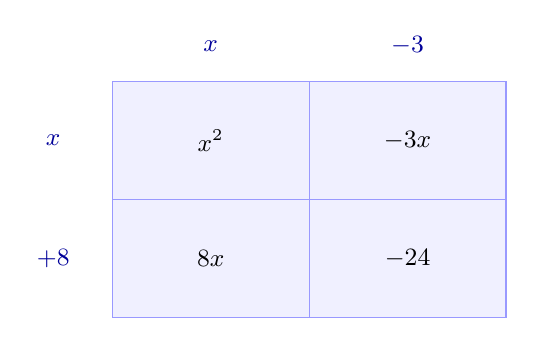
\begin{tikzpicture}[font=\small]
  \fill[blue!6] (0,0) rectangle (2.5,-1.5);
  \draw[blue!40] (0,0) rectangle (2.5,-1.5);
  \node at (1.25,-0.75) {$x^{2}$};
  \fill[blue!6] (2.5,0) rectangle (5,-1.5);
  \draw[blue!40] (2.5,0) rectangle (5,-1.5);
  \node at (3.75,-0.75) {$-3x$};
  \fill[blue!6] (0,-1.5) rectangle (2.5,-3);
  \draw[blue!40] (0,-1.5) rectangle (2.5,-3);
  \node at (1.25,-2.25) {$8x$};
  \fill[blue!6] (2.5,-1.5) rectangle (5,-3);
  \draw[blue!40] (2.5,-1.5) rectangle (5,-3);
  \node at (3.75,-2.25) {$-24$};
  \node[blue!60!black] at (1.25,0.45) {$x$};
  \node[blue!60!black] at (3.75,0.45) {$-3$};
  \node[blue!60!black] at (-0.75,-0.75) {$x$};
  \node[blue!60!black] at (-0.75,-2.25) {$+8$};
\end{tikzpicture} &
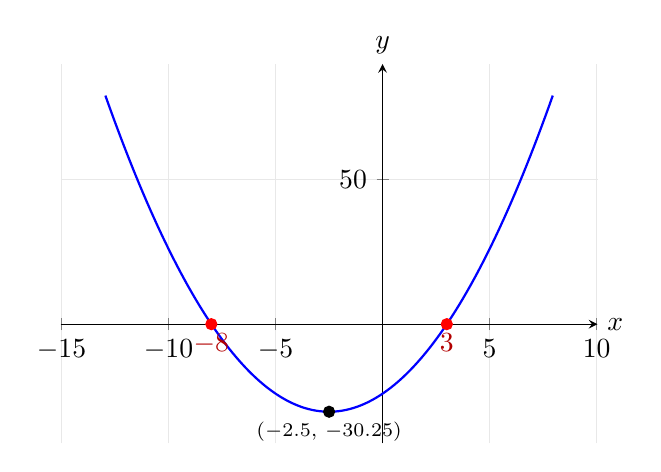
\begin{tikzpicture}
\begin{axis}[
  axis lines=middle, xlabel={$x$}, ylabel={$y$},
  width=8.4cm, height=6.4cm, grid=both, grid style={gray!18},
  enlargelimits=true, samples=120,
  domain=-12.95:7.95, every axis x label/.style={at={(ticklabel* cs:1)},anchor=west},
  every axis y label/.style={at={(ticklabel* cs:1)},anchor=south}]
  \addplot[blue, thick]{1*x^2 + 5*x - 24};
  \addplot[only marks, mark=*, red] coordinates {(-8,0)};
  \node[red!70!black, anchor=north] at (axis cs:-8,0) {$-8$};
  \addplot[only marks, mark=*, red] coordinates {(3,0)};
  \node[red!70!black, anchor=north] at (axis cs:3,0) {$3$};
  \addplot[only marks, mark=*, black] coordinates {(-2.5,-30.25)};
  \node[anchor=north] at (axis cs:-2.5,-30.25) {\scriptsize $(-2.5,\,-30.25)$};
\end{axis}
\end{tikzpicture}
\\[4pt]
{\small (a) Area / box model} & {\small (b) Graph $y=f(x)$ with its roots} \\
\end{tabular}
\end{center}
\vspace{2pt}\hrule\vspace{6pt}

\section*{Question 15 \quad {\normalfont\small\ttfamily qc1-015}}
\addcontentsline{toc}{section}{Q15. Monic ($a=1$)}
\nopagebreak
\begin{qbox}
Factorise: \( x^2 + x - 30 \)
\end{qbox}
\smallskip\noindent\textit{Type:} Monic ($a=1$) \hfill \textit{Marks:} 2 \quad \textit{Difficulty:} Foundation\\[2pt]
\subsection*{Worked solution}
\begin{enumerate}[leftmargin=1.6em,label=\textbf{Step \arabic*.}]
  \item Set up brackets.
  \[ (x \quad )(x \quad ) \]
  \par\smallskip{\small\itshape Monic quadratic.}
  \item Find numbers multiplying to \( -30 \) and adding to \( +1 \).
  \[ 6 \times (-5) = -30, \quad 6 + (-5) = 1 \]
  \par\smallskip{\small\itshape Factor pairs of 30: (1,30),(2,15),(3,10),(5,6). (5,6) differs by 1.}
  \item Write the answer.
  \[ (x + 6)(x - 5) \]
  \par\smallskip{\small\itshape Larger (6) takes the positive sign.}
\end{enumerate}
\begin{ansbox}\textbf{Final answer:}\quad \((x + 6)(x - 5)\)\end{ansbox}
\subsection*{Check by expanding}
Multiplying the brackets back out reproduces the original expression:
\[ x^{2} -5x +6x -30 \]
\subsection*{Visualising the factorisation}
\begin{center}
\begin{tabular}{cc}
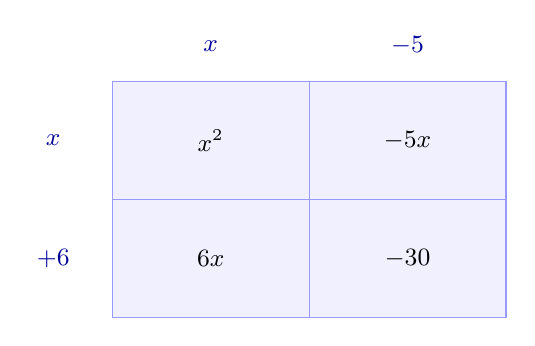
\begin{tikzpicture}[font=\small]
  \fill[blue!6] (0,0) rectangle (2.5,-1.5);
  \draw[blue!40] (0,0) rectangle (2.5,-1.5);
  \node at (1.25,-0.75) {$x^{2}$};
  \fill[blue!6] (2.5,0) rectangle (5,-1.5);
  \draw[blue!40] (2.5,0) rectangle (5,-1.5);
  \node at (3.75,-0.75) {$-5x$};
  \fill[blue!6] (0,-1.5) rectangle (2.5,-3);
  \draw[blue!40] (0,-1.5) rectangle (2.5,-3);
  \node at (1.25,-2.25) {$6x$};
  \fill[blue!6] (2.5,-1.5) rectangle (5,-3);
  \draw[blue!40] (2.5,-1.5) rectangle (5,-3);
  \node at (3.75,-2.25) {$-30$};
  \node[blue!60!black] at (1.25,0.45) {$x$};
  \node[blue!60!black] at (3.75,0.45) {$-5$};
  \node[blue!60!black] at (-0.75,-0.75) {$x$};
  \node[blue!60!black] at (-0.75,-2.25) {$+6$};
\end{tikzpicture} &
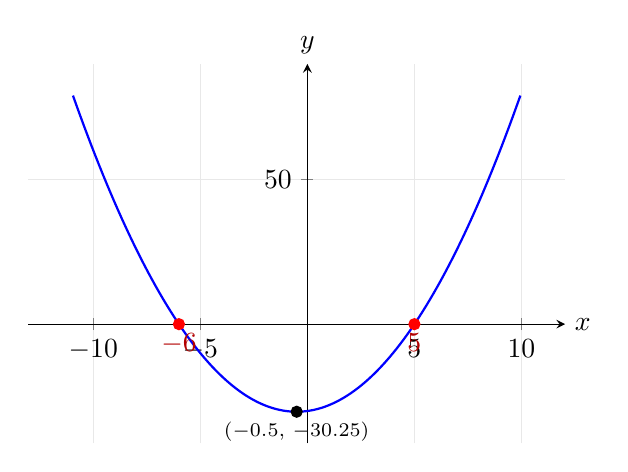
\begin{tikzpicture}
\begin{axis}[
  axis lines=middle, xlabel={$x$}, ylabel={$y$},
  width=8.4cm, height=6.4cm, grid=both, grid style={gray!18},
  enlargelimits=true, samples=120,
  domain=-10.95:9.95, every axis x label/.style={at={(ticklabel* cs:1)},anchor=west},
  every axis y label/.style={at={(ticklabel* cs:1)},anchor=south}]
  \addplot[blue, thick]{1*x^2 + 1*x - 30};
  \addplot[only marks, mark=*, red] coordinates {(-6,0)};
  \node[red!70!black, anchor=north] at (axis cs:-6,0) {$-6$};
  \addplot[only marks, mark=*, red] coordinates {(5,0)};
  \node[red!70!black, anchor=north] at (axis cs:5,0) {$5$};
  \addplot[only marks, mark=*, black] coordinates {(-0.5,-30.25)};
  \node[anchor=north] at (axis cs:-0.5,-30.25) {\scriptsize $(-0.5,\,-30.25)$};
\end{axis}
\end{tikzpicture}
\\[4pt]
{\small (a) Area / box model} & {\small (b) Graph $y=f(x)$ with its roots} \\
\end{tabular}
\end{center}
\vspace{2pt}\hrule\vspace{6pt}

\section*{Question 16 \quad {\normalfont\small\ttfamily qc1-016}}
\addcontentsline{toc}{section}{Q16. Monic ($a=1$)}
\nopagebreak
\begin{qbox}
Factorise: \( x^2 - 2x - 15 \)
\end{qbox}
\smallskip\noindent\textit{Type:} Monic ($a=1$) \hfill \textit{Marks:} 2 \quad \textit{Difficulty:} Foundation\\[2pt]
\subsection*{Worked solution}
\begin{enumerate}[leftmargin=1.6em,label=\textbf{Step \arabic*.}]
  \item Set up brackets.
  \[ (x \quad )(x \quad ) \]
  \par\smallskip{\small\itshape Monic quadratic.}
  \item Find numbers multiplying to \( -15 \) and adding to \( -2 \).
  \[ (-5) \times 3 = -15, \quad (-5) + 3 = -2 \]
  \par\smallskip{\small\itshape Opposite signs; the larger number is negative this time.}
  \item Write the answer.
  \[ (x - 5)(x + 3) \]
  \par\smallskip{\small\itshape Larger (5) takes the negative sign.}
\end{enumerate}
\begin{ansbox}\textbf{Final answer:}\quad \((x - 5)(x + 3)\)\end{ansbox}
\subsection*{Check by expanding}
Multiplying the brackets back out reproduces the original expression:
\[ x^{2} +3x -5x -15 \]
\subsection*{Visualising the factorisation}
\begin{center}
\begin{tabular}{cc}
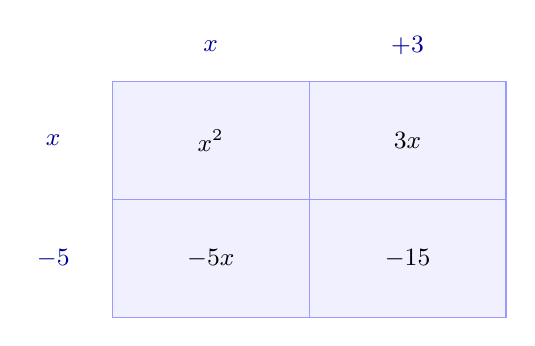
\begin{tikzpicture}[font=\small]
  \fill[blue!6] (0,0) rectangle (2.5,-1.5);
  \draw[blue!40] (0,0) rectangle (2.5,-1.5);
  \node at (1.25,-0.75) {$x^{2}$};
  \fill[blue!6] (2.5,0) rectangle (5,-1.5);
  \draw[blue!40] (2.5,0) rectangle (5,-1.5);
  \node at (3.75,-0.75) {$3x$};
  \fill[blue!6] (0,-1.5) rectangle (2.5,-3);
  \draw[blue!40] (0,-1.5) rectangle (2.5,-3);
  \node at (1.25,-2.25) {$-5x$};
  \fill[blue!6] (2.5,-1.5) rectangle (5,-3);
  \draw[blue!40] (2.5,-1.5) rectangle (5,-3);
  \node at (3.75,-2.25) {$-15$};
  \node[blue!60!black] at (1.25,0.45) {$x$};
  \node[blue!60!black] at (3.75,0.45) {$+3$};
  \node[blue!60!black] at (-0.75,-0.75) {$x$};
  \node[blue!60!black] at (-0.75,-2.25) {$-5$};
\end{tikzpicture} &
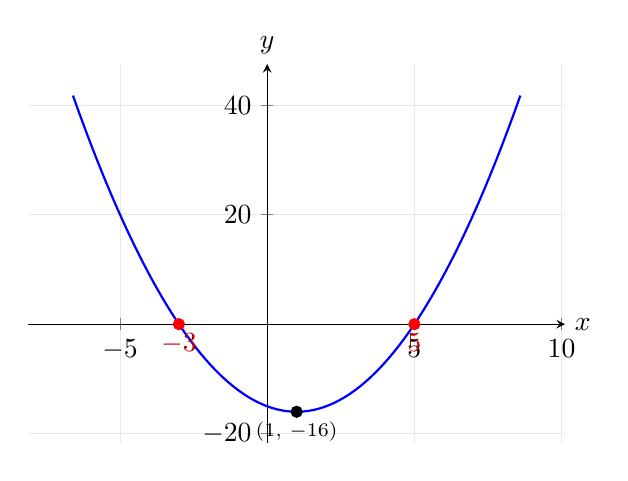
\begin{tikzpicture}
\begin{axis}[
  axis lines=middle, xlabel={$x$}, ylabel={$y$},
  width=8.4cm, height=6.4cm, grid=both, grid style={gray!18},
  enlargelimits=true, samples=120,
  domain=-6.6:8.6, every axis x label/.style={at={(ticklabel* cs:1)},anchor=west},
  every axis y label/.style={at={(ticklabel* cs:1)},anchor=south}]
  \addplot[blue, thick]{1*x^2 - 2*x - 15};
  \addplot[only marks, mark=*, red] coordinates {(5,0)};
  \node[red!70!black, anchor=north] at (axis cs:5,0) {$5$};
  \addplot[only marks, mark=*, red] coordinates {(-3,0)};
  \node[red!70!black, anchor=north] at (axis cs:-3,0) {$-3$};
  \addplot[only marks, mark=*, black] coordinates {(1,-16)};
  \node[anchor=north] at (axis cs:1,-16) {\scriptsize $(1,\,-16)$};
\end{axis}
\end{tikzpicture}
\\[4pt]
{\small (a) Area / box model} & {\small (b) Graph $y=f(x)$ with its roots} \\
\end{tabular}
\end{center}
\vspace{2pt}\hrule\vspace{6pt}

\section*{Question 17 \quad {\normalfont\small\ttfamily qc1-017}}
\addcontentsline{toc}{section}{Q17. Monic ($a=1$)}
\nopagebreak
\begin{qbox}
Factorise: \( x^2 - 3x - 10 \)
\end{qbox}
\smallskip\noindent\textit{Type:} Monic ($a=1$) \hfill \textit{Marks:} 2 \quad \textit{Difficulty:} Foundation\\[2pt]
\subsection*{Worked solution}
\begin{enumerate}[leftmargin=1.6em,label=\textbf{Step \arabic*.}]
  \item Set up brackets.
  \[ (x \quad )(x \quad ) \]
  \par\smallskip{\small\itshape Monic quadratic.}
  \item Find numbers multiplying to \( -10 \) and adding to \( -3 \).
  \[ (-5) \times 2 = -10, \quad (-5) + 2 = -3 \]
  \par\smallskip{\small\itshape Opposite signs; the larger factor (5) is negative.}
  \item Write the answer.
  \[ (x - 5)(x + 2) \]
  \par\smallskip{\small\itshape Larger goes with the negative sign.}
\end{enumerate}
\begin{ansbox}\textbf{Final answer:}\quad \((x - 5)(x + 2)\)\end{ansbox}
\subsection*{Check by expanding}
Multiplying the brackets back out reproduces the original expression:
\[ x^{2} +2x -5x -10 \]
\subsection*{Visualising the factorisation}
\begin{center}
\begin{tabular}{cc}
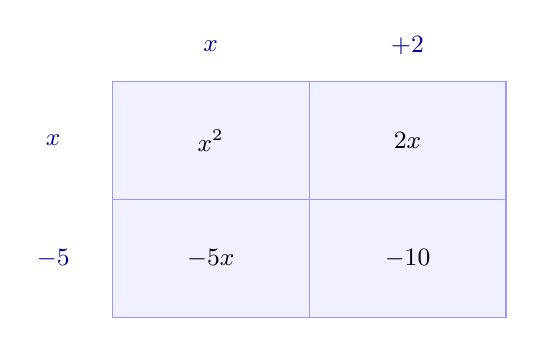
\begin{tikzpicture}[font=\small]
  \fill[blue!6] (0,0) rectangle (2.5,-1.5);
  \draw[blue!40] (0,0) rectangle (2.5,-1.5);
  \node at (1.25,-0.75) {$x^{2}$};
  \fill[blue!6] (2.5,0) rectangle (5,-1.5);
  \draw[blue!40] (2.5,0) rectangle (5,-1.5);
  \node at (3.75,-0.75) {$2x$};
  \fill[blue!6] (0,-1.5) rectangle (2.5,-3);
  \draw[blue!40] (0,-1.5) rectangle (2.5,-3);
  \node at (1.25,-2.25) {$-5x$};
  \fill[blue!6] (2.5,-1.5) rectangle (5,-3);
  \draw[blue!40] (2.5,-1.5) rectangle (5,-3);
  \node at (3.75,-2.25) {$-10$};
  \node[blue!60!black] at (1.25,0.45) {$x$};
  \node[blue!60!black] at (3.75,0.45) {$+2$};
  \node[blue!60!black] at (-0.75,-0.75) {$x$};
  \node[blue!60!black] at (-0.75,-2.25) {$-5$};
\end{tikzpicture} &
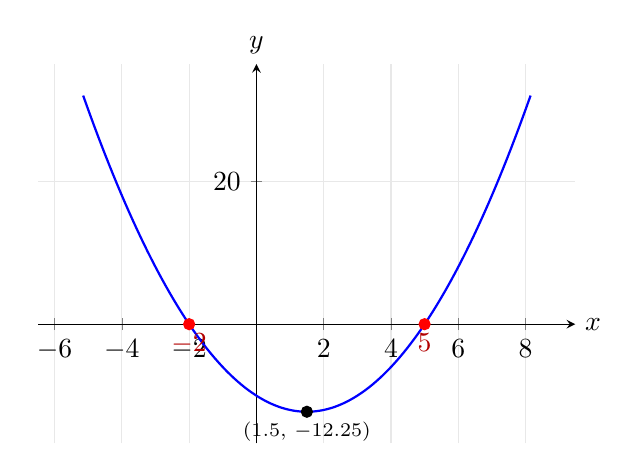
\begin{tikzpicture}
\begin{axis}[
  axis lines=middle, xlabel={$x$}, ylabel={$y$},
  width=8.4cm, height=6.4cm, grid=both, grid style={gray!18},
  enlargelimits=true, samples=120,
  domain=-5.15:8.15, every axis x label/.style={at={(ticklabel* cs:1)},anchor=west},
  every axis y label/.style={at={(ticklabel* cs:1)},anchor=south}]
  \addplot[blue, thick]{1*x^2 - 3*x - 10};
  \addplot[only marks, mark=*, red] coordinates {(5,0)};
  \node[red!70!black, anchor=north] at (axis cs:5,0) {$5$};
  \addplot[only marks, mark=*, red] coordinates {(-2,0)};
  \node[red!70!black, anchor=north] at (axis cs:-2,0) {$-2$};
  \addplot[only marks, mark=*, black] coordinates {(1.5,-12.25)};
  \node[anchor=north] at (axis cs:1.5,-12.25) {\scriptsize $(1.5,\,-12.25)$};
\end{axis}
\end{tikzpicture}
\\[4pt]
{\small (a) Area / box model} & {\small (b) Graph $y=f(x)$ with its roots} \\
\end{tabular}
\end{center}
\vspace{2pt}\hrule\vspace{6pt}

\section*{Question 18 \quad {\normalfont\small\ttfamily qc1-018}}
\addcontentsline{toc}{section}{Q18. Monic ($a=1$)}
\nopagebreak
\begin{qbox}
Factorise: \( x^2 - 5x - 14 \)
\end{qbox}
\smallskip\noindent\textit{Type:} Monic ($a=1$) \hfill \textit{Marks:} 2 \quad \textit{Difficulty:} Foundation\\[2pt]
\subsection*{Worked solution}
\begin{enumerate}[leftmargin=1.6em,label=\textbf{Step \arabic*.}]
  \item Set up brackets.
  \[ (x \quad )(x \quad ) \]
  \par\smallskip{\small\itshape Monic quadratic.}
  \item Find numbers multiplying to \( -14 \) and adding to \( -5 \).
  \[ (-7) \times 2 = -14, \quad (-7) + 2 = -5 \]
  \par\smallskip{\small\itshape Opposite signs with larger factor negative.}
  \item Write the answer.
  \[ (x - 7)(x + 2) \]
  \par\smallskip{\small\itshape Larger (7) is negative.}
\end{enumerate}
\begin{ansbox}\textbf{Final answer:}\quad \((x - 7)(x + 2)\)\end{ansbox}
\subsection*{Check by expanding}
Multiplying the brackets back out reproduces the original expression:
\[ x^{2} +2x -7x -14 \]
\subsection*{Visualising the factorisation}
\begin{center}
\begin{tabular}{cc}
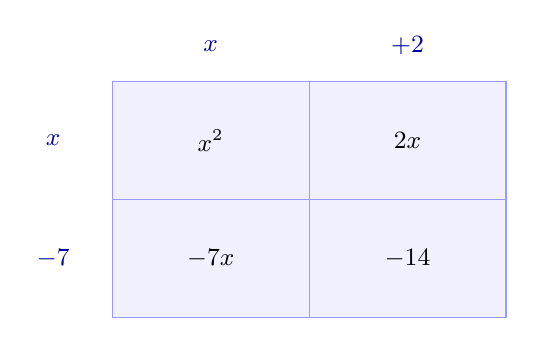
\begin{tikzpicture}[font=\small]
  \fill[blue!6] (0,0) rectangle (2.5,-1.5);
  \draw[blue!40] (0,0) rectangle (2.5,-1.5);
  \node at (1.25,-0.75) {$x^{2}$};
  \fill[blue!6] (2.5,0) rectangle (5,-1.5);
  \draw[blue!40] (2.5,0) rectangle (5,-1.5);
  \node at (3.75,-0.75) {$2x$};
  \fill[blue!6] (0,-1.5) rectangle (2.5,-3);
  \draw[blue!40] (0,-1.5) rectangle (2.5,-3);
  \node at (1.25,-2.25) {$-7x$};
  \fill[blue!6] (2.5,-1.5) rectangle (5,-3);
  \draw[blue!40] (2.5,-1.5) rectangle (5,-3);
  \node at (3.75,-2.25) {$-14$};
  \node[blue!60!black] at (1.25,0.45) {$x$};
  \node[blue!60!black] at (3.75,0.45) {$+2$};
  \node[blue!60!black] at (-0.75,-0.75) {$x$};
  \node[blue!60!black] at (-0.75,-2.25) {$-7$};
\end{tikzpicture} &
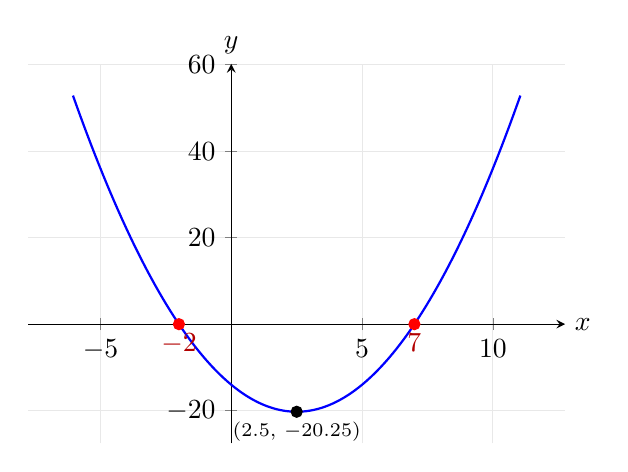
\begin{tikzpicture}
\begin{axis}[
  axis lines=middle, xlabel={$x$}, ylabel={$y$},
  width=8.4cm, height=6.4cm, grid=both, grid style={gray!18},
  enlargelimits=true, samples=120,
  domain=-6.05:11.05, every axis x label/.style={at={(ticklabel* cs:1)},anchor=west},
  every axis y label/.style={at={(ticklabel* cs:1)},anchor=south}]
  \addplot[blue, thick]{1*x^2 - 5*x - 14};
  \addplot[only marks, mark=*, red] coordinates {(7,0)};
  \node[red!70!black, anchor=north] at (axis cs:7,0) {$7$};
  \addplot[only marks, mark=*, red] coordinates {(-2,0)};
  \node[red!70!black, anchor=north] at (axis cs:-2,0) {$-2$};
  \addplot[only marks, mark=*, black] coordinates {(2.5,-20.25)};
  \node[anchor=north] at (axis cs:2.5,-20.25) {\scriptsize $(2.5,\,-20.25)$};
\end{axis}
\end{tikzpicture}
\\[4pt]
{\small (a) Area / box model} & {\small (b) Graph $y=f(x)$ with its roots} \\
\end{tabular}
\end{center}
\vspace{2pt}\hrule\vspace{6pt}

\section*{Question 19 \quad {\normalfont\small\ttfamily qc1-019}}
\addcontentsline{toc}{section}{Q19. Monic ($a=1$)}
\nopagebreak
\begin{qbox}
Factorise: \( x^2 - 6x - 16 \)
\end{qbox}
\smallskip\noindent\textit{Type:} Monic ($a=1$) \hfill \textit{Marks:} 2 \quad \textit{Difficulty:} Foundation\\[2pt]
\subsection*{Worked solution}
\begin{enumerate}[leftmargin=1.6em,label=\textbf{Step \arabic*.}]
  \item Set up brackets.
  \[ (x \quad )(x \quad ) \]
  \par\smallskip{\small\itshape Monic quadratic.}
  \item Find numbers multiplying to \( -16 \) and adding to \( -6 \).
  \[ (-8) \times 2 = -16, \quad (-8) + 2 = -6 \]
  \par\smallskip{\small\itshape Opposite signs with larger factor negative.}
  \item Write the answer.
  \[ (x - 8)(x + 2) \]
  \par\smallskip{\small\itshape Larger (8) is negative.}
\end{enumerate}
\begin{ansbox}\textbf{Final answer:}\quad \((x - 8)(x + 2)\)\end{ansbox}
\subsection*{Check by expanding}
Multiplying the brackets back out reproduces the original expression:
\[ x^{2} +2x -8x -16 \]
\subsection*{Visualising the factorisation}
\begin{center}
\begin{tabular}{cc}
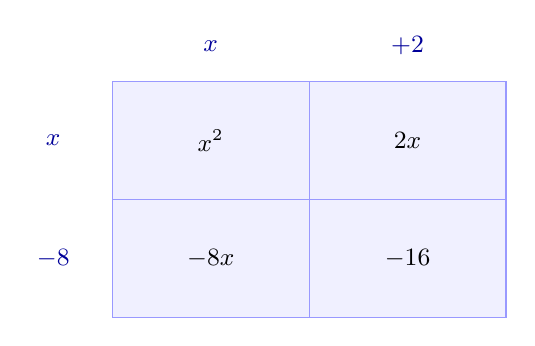
\begin{tikzpicture}[font=\small]
  \fill[blue!6] (0,0) rectangle (2.5,-1.5);
  \draw[blue!40] (0,0) rectangle (2.5,-1.5);
  \node at (1.25,-0.75) {$x^{2}$};
  \fill[blue!6] (2.5,0) rectangle (5,-1.5);
  \draw[blue!40] (2.5,0) rectangle (5,-1.5);
  \node at (3.75,-0.75) {$2x$};
  \fill[blue!6] (0,-1.5) rectangle (2.5,-3);
  \draw[blue!40] (0,-1.5) rectangle (2.5,-3);
  \node at (1.25,-2.25) {$-8x$};
  \fill[blue!6] (2.5,-1.5) rectangle (5,-3);
  \draw[blue!40] (2.5,-1.5) rectangle (5,-3);
  \node at (3.75,-2.25) {$-16$};
  \node[blue!60!black] at (1.25,0.45) {$x$};
  \node[blue!60!black] at (3.75,0.45) {$+2$};
  \node[blue!60!black] at (-0.75,-0.75) {$x$};
  \node[blue!60!black] at (-0.75,-2.25) {$-8$};
\end{tikzpicture} &
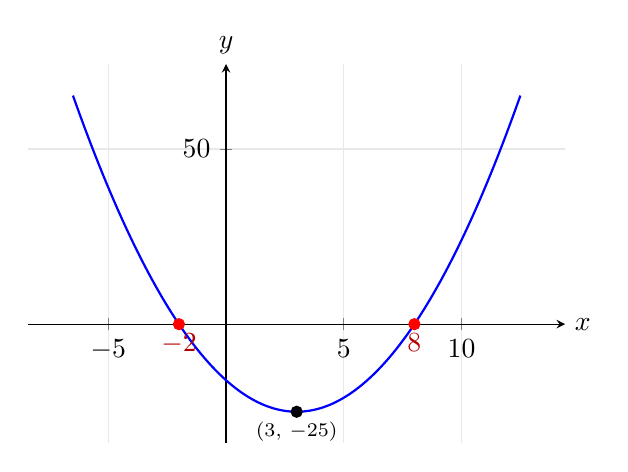
\begin{tikzpicture}
\begin{axis}[
  axis lines=middle, xlabel={$x$}, ylabel={$y$},
  width=8.4cm, height=6.4cm, grid=both, grid style={gray!18},
  enlargelimits=true, samples=120,
  domain=-6.5:12.5, every axis x label/.style={at={(ticklabel* cs:1)},anchor=west},
  every axis y label/.style={at={(ticklabel* cs:1)},anchor=south}]
  \addplot[blue, thick]{1*x^2 - 6*x - 16};
  \addplot[only marks, mark=*, red] coordinates {(8,0)};
  \node[red!70!black, anchor=north] at (axis cs:8,0) {$8$};
  \addplot[only marks, mark=*, red] coordinates {(-2,0)};
  \node[red!70!black, anchor=north] at (axis cs:-2,0) {$-2$};
  \addplot[only marks, mark=*, black] coordinates {(3,-25)};
  \node[anchor=north] at (axis cs:3,-25) {\scriptsize $(3,\,-25)$};
\end{axis}
\end{tikzpicture}
\\[4pt]
{\small (a) Area / box model} & {\small (b) Graph $y=f(x)$ with its roots} \\
\end{tabular}
\end{center}
\vspace{2pt}\hrule\vspace{6pt}

\section*{Question 20 \quad {\normalfont\small\ttfamily qc1-020}}
\addcontentsline{toc}{section}{Q20. Monic ($a=1$)}
\nopagebreak
\begin{qbox}
Factorise: \( x^2 - 4x - 32 \)
\end{qbox}
\smallskip\noindent\textit{Type:} Monic ($a=1$) \hfill \textit{Marks:} 2 \quad \textit{Difficulty:} Foundation\\[2pt]
\subsection*{Worked solution}
\begin{enumerate}[leftmargin=1.6em,label=\textbf{Step \arabic*.}]
  \item Set up brackets.
  \[ (x \quad )(x \quad ) \]
  \par\smallskip{\small\itshape Monic quadratic.}
  \item Find numbers multiplying to \( -32 \) and adding to \( -4 \).
  \[ (-8) \times 4 = -32, \quad (-8) + 4 = -4 \]
  \par\smallskip{\small\itshape Factor pairs of 32: (1,32),(2,16),(4,8). (4,8) differs by 4.}
  \item Write the answer.
  \[ (x - 8)(x + 4) \]
  \par\smallskip{\small\itshape Larger (8) is negative.}
\end{enumerate}
\begin{ansbox}\textbf{Final answer:}\quad \((x - 8)(x + 4)\)\end{ansbox}
\subsection*{Check by expanding}
Multiplying the brackets back out reproduces the original expression:
\[ x^{2} +4x -8x -32 \]
\subsection*{Visualising the factorisation}
\begin{center}
\begin{tabular}{cc}
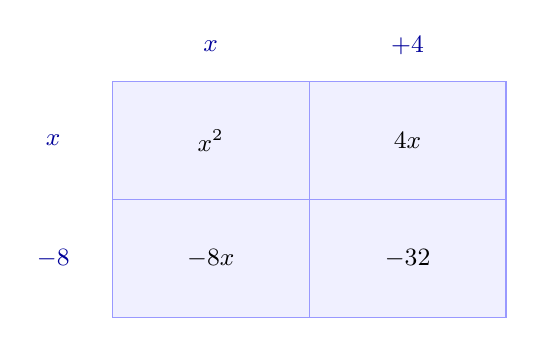
\begin{tikzpicture}[font=\small]
  \fill[blue!6] (0,0) rectangle (2.5,-1.5);
  \draw[blue!40] (0,0) rectangle (2.5,-1.5);
  \node at (1.25,-0.75) {$x^{2}$};
  \fill[blue!6] (2.5,0) rectangle (5,-1.5);
  \draw[blue!40] (2.5,0) rectangle (5,-1.5);
  \node at (3.75,-0.75) {$4x$};
  \fill[blue!6] (0,-1.5) rectangle (2.5,-3);
  \draw[blue!40] (0,-1.5) rectangle (2.5,-3);
  \node at (1.25,-2.25) {$-8x$};
  \fill[blue!6] (2.5,-1.5) rectangle (5,-3);
  \draw[blue!40] (2.5,-1.5) rectangle (5,-3);
  \node at (3.75,-2.25) {$-32$};
  \node[blue!60!black] at (1.25,0.45) {$x$};
  \node[blue!60!black] at (3.75,0.45) {$+4$};
  \node[blue!60!black] at (-0.75,-0.75) {$x$};
  \node[blue!60!black] at (-0.75,-2.25) {$-8$};
\end{tikzpicture} &
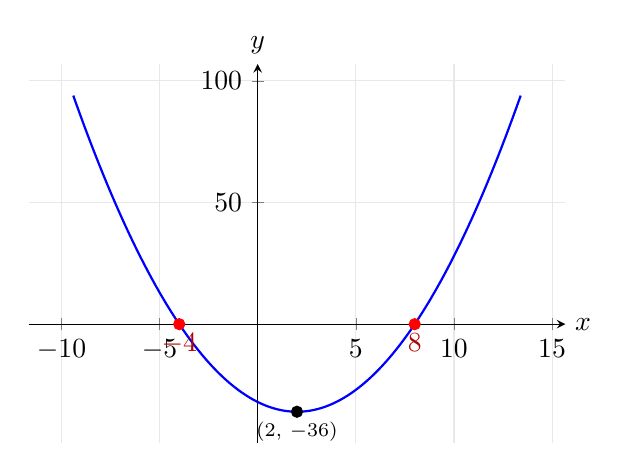
\begin{tikzpicture}
\begin{axis}[
  axis lines=middle, xlabel={$x$}, ylabel={$y$},
  width=8.4cm, height=6.4cm, grid=both, grid style={gray!18},
  enlargelimits=true, samples=120,
  domain=-9.4:13.4, every axis x label/.style={at={(ticklabel* cs:1)},anchor=west},
  every axis y label/.style={at={(ticklabel* cs:1)},anchor=south}]
  \addplot[blue, thick]{1*x^2 - 4*x - 32};
  \addplot[only marks, mark=*, red] coordinates {(8,0)};
  \node[red!70!black, anchor=north] at (axis cs:8,0) {$8$};
  \addplot[only marks, mark=*, red] coordinates {(-4,0)};
  \node[red!70!black, anchor=north] at (axis cs:-4,0) {$-4$};
  \addplot[only marks, mark=*, black] coordinates {(2,-36)};
  \node[anchor=north] at (axis cs:2,-36) {\scriptsize $(2,\,-36)$};
\end{axis}
\end{tikzpicture}
\\[4pt]
{\small (a) Area / box model} & {\small (b) Graph $y=f(x)$ with its roots} \\
\end{tabular}
\end{center}
\vspace{2pt}\hrule\vspace{6pt}

\section*{Question 21 \quad {\normalfont\small\ttfamily qc1-021}}
\addcontentsline{toc}{section}{Q21. Perfect square}
\nopagebreak
\begin{qbox}
Factorise: \( x^2 + 8x + 16 \)
\end{qbox}
\smallskip\noindent\textit{Type:} Perfect square \hfill \textit{Marks:} 2 \quad \textit{Difficulty:} Foundation\\[2pt]
\subsection*{Worked solution}
\begin{enumerate}[leftmargin=1.6em,label=\textbf{Step \arabic*.}]
  \item Set up brackets.
  \[ (x \quad )(x \quad ) \]
  \par\smallskip{\small\itshape Monic quadratic.}
  \item Find numbers multiplying to 16 and adding to 8.
  \[ 4 \times 4 = 16, \quad 4 + 4 = 8 \]
  \par\smallskip{\small\itshape A repeated factor of 4 works - this is a perfect square.}
  \item Write the answer.
  \[ (x + 4)(x + 4) = (x + 4)^2 \]
  \par\smallskip{\small\itshape Repeated factor gives a perfect square.}
\end{enumerate}
\begin{ansbox}\textbf{Final answer:}\quad \((x + 4)^2\)\end{ansbox}
\subsection*{Check by expanding}
Multiplying the brackets back out reproduces the original expression:
\[ x^{2} +4x +4x +16 \]
\subsection*{Visualising the factorisation}
\begin{center}
\begin{tabular}{cc}
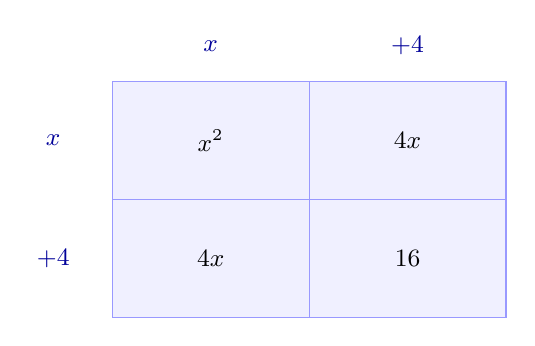
\begin{tikzpicture}[font=\small]
  \fill[blue!6] (0,0) rectangle (2.5,-1.5);
  \draw[blue!40] (0,0) rectangle (2.5,-1.5);
  \node at (1.25,-0.75) {$x^{2}$};
  \fill[blue!6] (2.5,0) rectangle (5,-1.5);
  \draw[blue!40] (2.5,0) rectangle (5,-1.5);
  \node at (3.75,-0.75) {$4x$};
  \fill[blue!6] (0,-1.5) rectangle (2.5,-3);
  \draw[blue!40] (0,-1.5) rectangle (2.5,-3);
  \node at (1.25,-2.25) {$4x$};
  \fill[blue!6] (2.5,-1.5) rectangle (5,-3);
  \draw[blue!40] (2.5,-1.5) rectangle (5,-3);
  \node at (3.75,-2.25) {$16$};
  \node[blue!60!black] at (1.25,0.45) {$x$};
  \node[blue!60!black] at (3.75,0.45) {$+4$};
  \node[blue!60!black] at (-0.75,-0.75) {$x$};
  \node[blue!60!black] at (-0.75,-2.25) {$+4$};
\end{tikzpicture} &
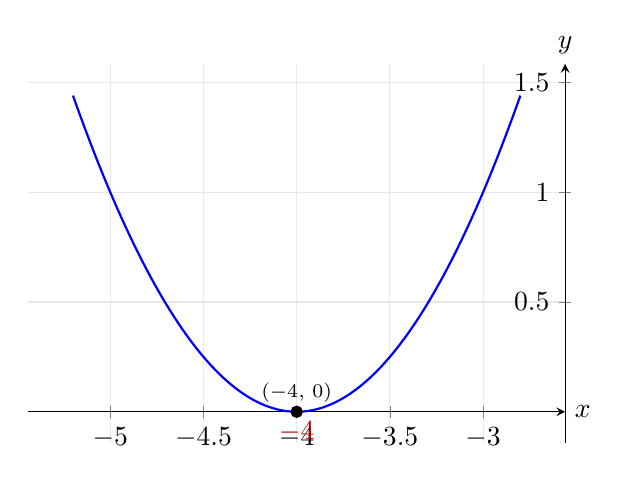
\begin{tikzpicture}
\begin{axis}[
  axis lines=middle, xlabel={$x$}, ylabel={$y$},
  width=8.4cm, height=6.4cm, grid=both, grid style={gray!18},
  enlargelimits=true, samples=120,
  domain=-5.2:-2.8, every axis x label/.style={at={(ticklabel* cs:1)},anchor=west},
  every axis y label/.style={at={(ticklabel* cs:1)},anchor=south}]
  \addplot[blue, thick]{1*x^2 + 8*x + 16};
  \addplot[only marks, mark=*, red] coordinates {(-4,0)};
  \node[red!70!black, anchor=north] at (axis cs:-4,0) {$-4$};
  \addplot[only marks, mark=*, black] coordinates {(-4,0)};
  \node[anchor=south] at (axis cs:-4,0) {\scriptsize $(-4,\,0)$};
\end{axis}
\end{tikzpicture}
\\[4pt]
{\small (a) Area / box model} & {\small (b) Graph $y=f(x)$ with its roots} \\
\end{tabular}
\end{center}
\vspace{2pt}\hrule\vspace{6pt}

\section*{Question 22 \quad {\normalfont\small\ttfamily qc1-022}}
\addcontentsline{toc}{section}{Q22. Perfect square}
\nopagebreak
\begin{qbox}
Factorise: \( x^2 - 10x + 25 \)
\end{qbox}
\smallskip\noindent\textit{Type:} Perfect square \hfill \textit{Marks:} 2 \quad \textit{Difficulty:} Foundation\\[2pt]
\subsection*{Worked solution}
\begin{enumerate}[leftmargin=1.6em,label=\textbf{Step \arabic*.}]
  \item Set up brackets.
  \[ (x \quad )(x \quad ) \]
  \par\smallskip{\small\itshape Monic quadratic.}
  \item Find numbers multiplying to 25 and adding to \( -10 \).
  \[ (-5) \times (-5) = 25, \quad (-5) + (-5) = -10 \]
  \par\smallskip{\small\itshape Repeated factor of \( -5 \).}
  \item Write the answer.
  \[ (x - 5)^2 \]
  \par\smallskip{\small\itshape Perfect square.}
\end{enumerate}
\begin{ansbox}\textbf{Final answer:}\quad \((x - 5)^2\)\end{ansbox}
\subsection*{Check by expanding}
Multiplying the brackets back out reproduces the original expression:
\[ x^{2} -5x -5x +25 \]
\subsection*{Visualising the factorisation}
\begin{center}
\begin{tabular}{cc}
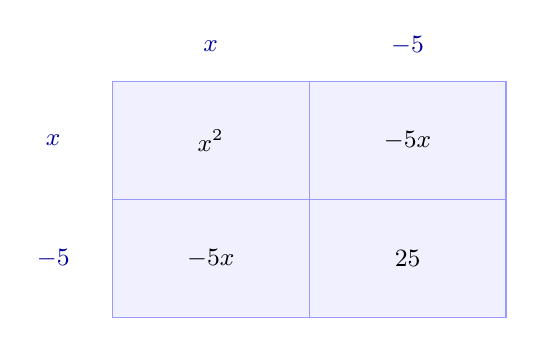
\begin{tikzpicture}[font=\small]
  \fill[blue!6] (0,0) rectangle (2.5,-1.5);
  \draw[blue!40] (0,0) rectangle (2.5,-1.5);
  \node at (1.25,-0.75) {$x^{2}$};
  \fill[blue!6] (2.5,0) rectangle (5,-1.5);
  \draw[blue!40] (2.5,0) rectangle (5,-1.5);
  \node at (3.75,-0.75) {$-5x$};
  \fill[blue!6] (0,-1.5) rectangle (2.5,-3);
  \draw[blue!40] (0,-1.5) rectangle (2.5,-3);
  \node at (1.25,-2.25) {$-5x$};
  \fill[blue!6] (2.5,-1.5) rectangle (5,-3);
  \draw[blue!40] (2.5,-1.5) rectangle (5,-3);
  \node at (3.75,-2.25) {$25$};
  \node[blue!60!black] at (1.25,0.45) {$x$};
  \node[blue!60!black] at (3.75,0.45) {$-5$};
  \node[blue!60!black] at (-0.75,-0.75) {$x$};
  \node[blue!60!black] at (-0.75,-2.25) {$-5$};
\end{tikzpicture} &
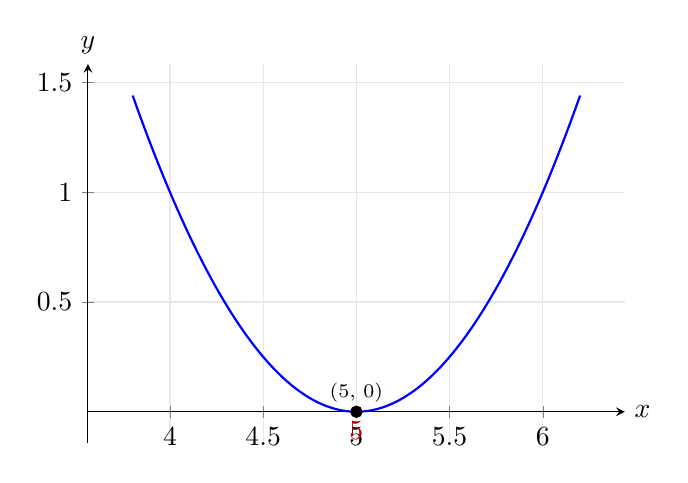
\begin{tikzpicture}
\begin{axis}[
  axis lines=middle, xlabel={$x$}, ylabel={$y$},
  width=8.4cm, height=6.4cm, grid=both, grid style={gray!18},
  enlargelimits=true, samples=120,
  domain=3.8:6.2, every axis x label/.style={at={(ticklabel* cs:1)},anchor=west},
  every axis y label/.style={at={(ticklabel* cs:1)},anchor=south}]
  \addplot[blue, thick]{1*x^2 - 10*x + 25};
  \addplot[only marks, mark=*, red] coordinates {(5,0)};
  \node[red!70!black, anchor=north] at (axis cs:5,0) {$5$};
  \addplot[only marks, mark=*, black] coordinates {(5,0)};
  \node[anchor=south] at (axis cs:5,0) {\scriptsize $(5,\,0)$};
\end{axis}
\end{tikzpicture}
\\[4pt]
{\small (a) Area / box model} & {\small (b) Graph $y=f(x)$ with its roots} \\
\end{tabular}
\end{center}
\vspace{2pt}\hrule\vspace{6pt}

\section*{Question 23 \quad {\normalfont\small\ttfamily qc1-023}}
\addcontentsline{toc}{section}{Q23. Perfect square}
\nopagebreak
\begin{qbox}
Factorise: \( x^2 + 12x + 36 \)
\end{qbox}
\smallskip\noindent\textit{Type:} Perfect square \hfill \textit{Marks:} 2 \quad \textit{Difficulty:} Foundation\\[2pt]
\subsection*{Worked solution}
\begin{enumerate}[leftmargin=1.6em,label=\textbf{Step \arabic*.}]
  \item Set up brackets.
  \[ (x \quad )(x \quad ) \]
  \par\smallskip{\small\itshape Monic quadratic.}
  \item Find numbers multiplying to 36 and adding to 12.
  \[ 6 \times 6 = 36, \quad 6 + 6 = 12 \]
  \par\smallskip{\small\itshape Repeated factor of 6.}
  \item Write the answer.
  \[ (x + 6)^2 \]
  \par\smallskip{\small\itshape Perfect square.}
\end{enumerate}
\begin{ansbox}\textbf{Final answer:}\quad \((x + 6)^2\)\end{ansbox}
\subsection*{Check by expanding}
Multiplying the brackets back out reproduces the original expression:
\[ x^{2} +6x +6x +36 \]
\subsection*{Visualising the factorisation}
\begin{center}
\begin{tabular}{cc}
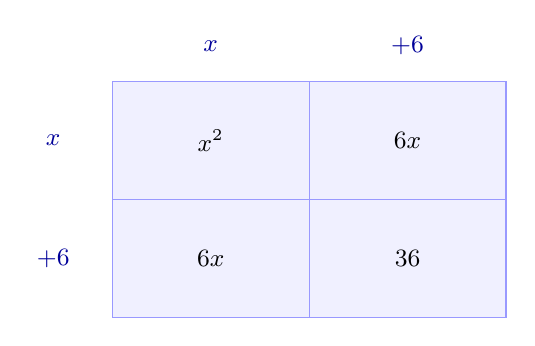
\begin{tikzpicture}[font=\small]
  \fill[blue!6] (0,0) rectangle (2.5,-1.5);
  \draw[blue!40] (0,0) rectangle (2.5,-1.5);
  \node at (1.25,-0.75) {$x^{2}$};
  \fill[blue!6] (2.5,0) rectangle (5,-1.5);
  \draw[blue!40] (2.5,0) rectangle (5,-1.5);
  \node at (3.75,-0.75) {$6x$};
  \fill[blue!6] (0,-1.5) rectangle (2.5,-3);
  \draw[blue!40] (0,-1.5) rectangle (2.5,-3);
  \node at (1.25,-2.25) {$6x$};
  \fill[blue!6] (2.5,-1.5) rectangle (5,-3);
  \draw[blue!40] (2.5,-1.5) rectangle (5,-3);
  \node at (3.75,-2.25) {$36$};
  \node[blue!60!black] at (1.25,0.45) {$x$};
  \node[blue!60!black] at (3.75,0.45) {$+6$};
  \node[blue!60!black] at (-0.75,-0.75) {$x$};
  \node[blue!60!black] at (-0.75,-2.25) {$+6$};
\end{tikzpicture} &
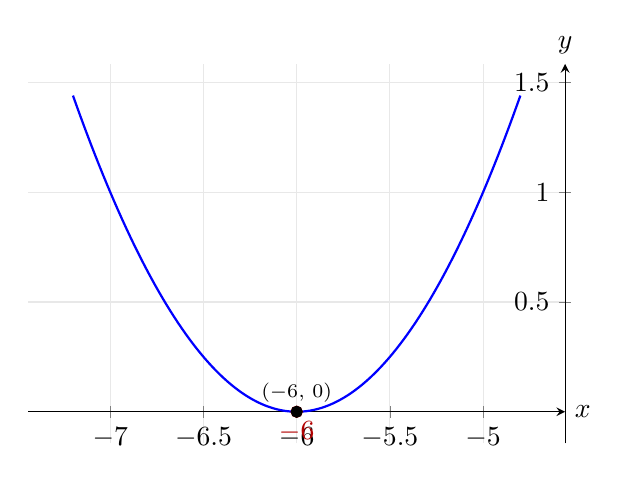
\begin{tikzpicture}
\begin{axis}[
  axis lines=middle, xlabel={$x$}, ylabel={$y$},
  width=8.4cm, height=6.4cm, grid=both, grid style={gray!18},
  enlargelimits=true, samples=120,
  domain=-7.2:-4.8, every axis x label/.style={at={(ticklabel* cs:1)},anchor=west},
  every axis y label/.style={at={(ticklabel* cs:1)},anchor=south}]
  \addplot[blue, thick]{1*x^2 + 12*x + 36};
  \addplot[only marks, mark=*, red] coordinates {(-6,0)};
  \node[red!70!black, anchor=north] at (axis cs:-6,0) {$-6$};
  \addplot[only marks, mark=*, black] coordinates {(-6,0)};
  \node[anchor=south] at (axis cs:-6,0) {\scriptsize $(-6,\,0)$};
\end{axis}
\end{tikzpicture}
\\[4pt]
{\small (a) Area / box model} & {\small (b) Graph $y=f(x)$ with its roots} \\
\end{tabular}
\end{center}
\vspace{2pt}\hrule\vspace{6pt}

\section*{Question 24 \quad {\normalfont\small\ttfamily qc1-024}}
\addcontentsline{toc}{section}{Q24. Perfect square}
\nopagebreak
\begin{qbox}
Factorise: \( x^2 - 14x + 49 \)
\end{qbox}
\smallskip\noindent\textit{Type:} Perfect square \hfill \textit{Marks:} 2 \quad \textit{Difficulty:} Foundation\\[2pt]
\subsection*{Worked solution}
\begin{enumerate}[leftmargin=1.6em,label=\textbf{Step \arabic*.}]
  \item Set up brackets.
  \[ (x \quad )(x \quad ) \]
  \par\smallskip{\small\itshape Monic quadratic.}
  \item Find numbers multiplying to 49 and adding to \( -14 \).
  \[ (-7) \times (-7) = 49, \quad (-7) + (-7) = -14 \]
  \par\smallskip{\small\itshape Repeated factor of \( -7 \).}
  \item Write the answer.
  \[ (x - 7)^2 \]
  \par\smallskip{\small\itshape Perfect square.}
\end{enumerate}
\begin{ansbox}\textbf{Final answer:}\quad \((x - 7)^2\)\end{ansbox}
\subsection*{Check by expanding}
Multiplying the brackets back out reproduces the original expression:
\[ x^{2} -7x -7x +49 \]
\subsection*{Visualising the factorisation}
\begin{center}
\begin{tabular}{cc}
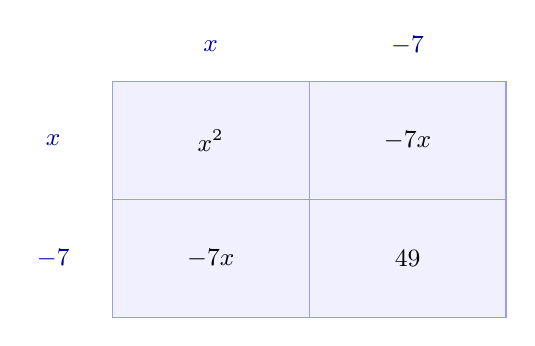
\begin{tikzpicture}[font=\small]
  \fill[blue!6] (0,0) rectangle (2.5,-1.5);
  \draw[blue!40] (0,0) rectangle (2.5,-1.5);
  \node at (1.25,-0.75) {$x^{2}$};
  \fill[blue!6] (2.5,0) rectangle (5,-1.5);
  \draw[blue!40] (2.5,0) rectangle (5,-1.5);
  \node at (3.75,-0.75) {$-7x$};
  \fill[blue!6] (0,-1.5) rectangle (2.5,-3);
  \draw[blue!40] (0,-1.5) rectangle (2.5,-3);
  \node at (1.25,-2.25) {$-7x$};
  \fill[blue!6] (2.5,-1.5) rectangle (5,-3);
  \draw[blue!40] (2.5,-1.5) rectangle (5,-3);
  \node at (3.75,-2.25) {$49$};
  \node[blue!60!black] at (1.25,0.45) {$x$};
  \node[blue!60!black] at (3.75,0.45) {$-7$};
  \node[blue!60!black] at (-0.75,-0.75) {$x$};
  \node[blue!60!black] at (-0.75,-2.25) {$-7$};
\end{tikzpicture} &
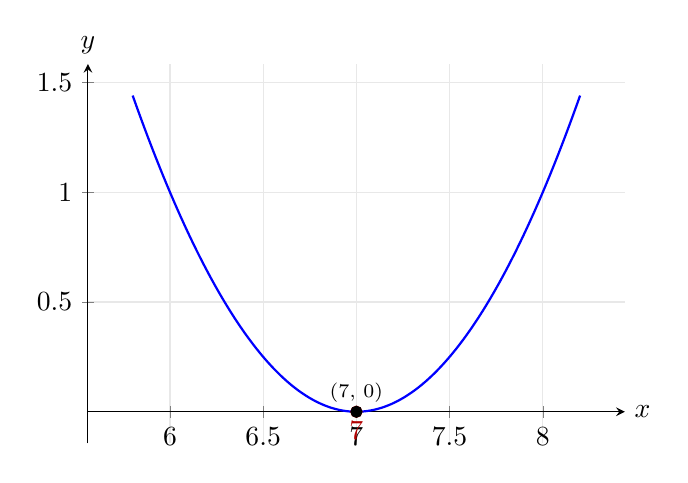
\begin{tikzpicture}
\begin{axis}[
  axis lines=middle, xlabel={$x$}, ylabel={$y$},
  width=8.4cm, height=6.4cm, grid=both, grid style={gray!18},
  enlargelimits=true, samples=120,
  domain=5.8:8.2, every axis x label/.style={at={(ticklabel* cs:1)},anchor=west},
  every axis y label/.style={at={(ticklabel* cs:1)},anchor=south}]
  \addplot[blue, thick]{1*x^2 - 14*x + 49};
  \addplot[only marks, mark=*, red] coordinates {(7,0)};
  \node[red!70!black, anchor=north] at (axis cs:7,0) {$7$};
  \addplot[only marks, mark=*, black] coordinates {(7,0)};
  \node[anchor=south] at (axis cs:7,0) {\scriptsize $(7,\,0)$};
\end{axis}
\end{tikzpicture}
\\[4pt]
{\small (a) Area / box model} & {\small (b) Graph $y=f(x)$ with its roots} \\
\end{tabular}
\end{center}
\vspace{2pt}\hrule\vspace{6pt}

\section*{Question 25 \quad {\normalfont\small\ttfamily qc1-025}}
\addcontentsline{toc}{section}{Q25. Difference of two squares}
\nopagebreak
\begin{qbox}
Factorise: \( x^2 - 25 \)
\end{qbox}
\smallskip\noindent\textit{Type:} Difference of two squares \hfill \textit{Marks:} 2 \quad \textit{Difficulty:} Foundation\\[2pt]
\subsection*{Worked solution}
\begin{enumerate}[leftmargin=1.6em,label=\textbf{Step \arabic*.}]
  \item Recognise the difference of two squares.
  \[ x^2 - 25 = x^2 - 5^2 \]
  \par\smallskip{\small\itshape Both \( x^2 \) and 25 are perfect squares separated by a minus sign.}
  \item Apply \( a^2 - b^2 = (a - b)(a + b) \).
  \[ (x - 5)(x + 5) \]
  \par\smallskip{\small\itshape Replace \( a \) with \( x \) and \( b \) with 5.}
\end{enumerate}
\begin{ansbox}\textbf{Final answer:}\quad \((x - 5)(x + 5)\)\end{ansbox}
\subsection*{Check by expanding}
Multiplying the brackets back out reproduces the original expression:
\[ x^{2} +5x -5x -25 \]
\subsection*{Visualising the factorisation}
\begin{center}
\begin{tabular}{cc}
\begin{tikzpicture}[font=\small]
  \fill[blue!6] (0,0) rectangle (2.5,-1.5);
  \draw[blue!40] (0,0) rectangle (2.5,-1.5);
  \node at (1.25,-0.75) {$x^{2}$};
  \fill[blue!6] (2.5,0) rectangle (5,-1.5);
  \draw[blue!40] (2.5,0) rectangle (5,-1.5);
  \node at (3.75,-0.75) {$5x$};
  \fill[blue!6] (0,-1.5) rectangle (2.5,-3);
  \draw[blue!40] (0,-1.5) rectangle (2.5,-3);
  \node at (1.25,-2.25) {$-5x$};
  \fill[blue!6] (2.5,-1.5) rectangle (5,-3);
  \draw[blue!40] (2.5,-1.5) rectangle (5,-3);
  \node at (3.75,-2.25) {$-25$};
  \node[blue!60!black] at (1.25,0.45) {$x$};
  \node[blue!60!black] at (3.75,0.45) {$+5$};
  \node[blue!60!black] at (-0.75,-0.75) {$x$};
  \node[blue!60!black] at (-0.75,-2.25) {$-5$};
\end{tikzpicture} &
\begin{tikzpicture}
\begin{axis}[
  axis lines=middle, xlabel={$x$}, ylabel={$y$},
  width=8.4cm, height=6.4cm, grid=both, grid style={gray!18},
  enlargelimits=true, samples=120,
  domain=-9.5:9.5, every axis x label/.style={at={(ticklabel* cs:1)},anchor=west},
  every axis y label/.style={at={(ticklabel* cs:1)},anchor=south}]
  \addplot[blue, thick]{1*x^2 + 0*x - 25};
  \addplot[only marks, mark=*, red] coordinates {(5,0)};
  \node[red!70!black, anchor=north] at (axis cs:5,0) {$5$};
  \addplot[only marks, mark=*, red] coordinates {(-5,0)};
  \node[red!70!black, anchor=north] at (axis cs:-5,0) {$-5$};
  \addplot[only marks, mark=*, black] coordinates {(0,-25)};
  \node[anchor=north] at (axis cs:0,-25) {\scriptsize $(0,\,-25)$};
\end{axis}
\end{tikzpicture}
\\[4pt]
{\small (a) Area / box model} & {\small (b) Graph $y=f(x)$ with its roots} \\
\end{tabular}
\end{center}
\vspace{2pt}\hrule\vspace{6pt}

\section*{Question 26 \quad {\normalfont\small\ttfamily qc1-026}}
\addcontentsline{toc}{section}{Q26. Difference of two squares}
\nopagebreak
\begin{qbox}
Factorise: \( x^2 - 64 \)
\end{qbox}
\smallskip\noindent\textit{Type:} Difference of two squares \hfill \textit{Marks:} 2 \quad \textit{Difficulty:} Foundation\\[2pt]
\subsection*{Worked solution}
\begin{enumerate}[leftmargin=1.6em,label=\textbf{Step \arabic*.}]
  \item Recognise the difference of two squares.
  \[ x^2 - 64 = x^2 - 8^2 \]
  \par\smallskip{\small\itshape 64 = \( 8^2 \).}
  \item Apply the difference of two squares formula.
  \[ (x - 8)(x + 8) \]
  \par\smallskip{\small\itshape One bracket with a minus, one with a plus.}
\end{enumerate}
\begin{ansbox}\textbf{Final answer:}\quad \((x - 8)(x + 8)\)\end{ansbox}
\subsection*{Check by expanding}
Multiplying the brackets back out reproduces the original expression:
\[ x^{2} +8x -8x -64 \]
\subsection*{Visualising the factorisation}
\begin{center}
\begin{tabular}{cc}
\begin{tikzpicture}[font=\small]
  \fill[blue!6] (0,0) rectangle (2.5,-1.5);
  \draw[blue!40] (0,0) rectangle (2.5,-1.5);
  \node at (1.25,-0.75) {$x^{2}$};
  \fill[blue!6] (2.5,0) rectangle (5,-1.5);
  \draw[blue!40] (2.5,0) rectangle (5,-1.5);
  \node at (3.75,-0.75) {$8x$};
  \fill[blue!6] (0,-1.5) rectangle (2.5,-3);
  \draw[blue!40] (0,-1.5) rectangle (2.5,-3);
  \node at (1.25,-2.25) {$-8x$};
  \fill[blue!6] (2.5,-1.5) rectangle (5,-3);
  \draw[blue!40] (2.5,-1.5) rectangle (5,-3);
  \node at (3.75,-2.25) {$-64$};
  \node[blue!60!black] at (1.25,0.45) {$x$};
  \node[blue!60!black] at (3.75,0.45) {$+8$};
  \node[blue!60!black] at (-0.75,-0.75) {$x$};
  \node[blue!60!black] at (-0.75,-2.25) {$-8$};
\end{tikzpicture} &
\begin{tikzpicture}
\begin{axis}[
  axis lines=middle, xlabel={$x$}, ylabel={$y$},
  width=8.4cm, height=6.4cm, grid=both, grid style={gray!18},
  enlargelimits=true, samples=120,
  domain=-15.2:15.2, every axis x label/.style={at={(ticklabel* cs:1)},anchor=west},
  every axis y label/.style={at={(ticklabel* cs:1)},anchor=south}]
  \addplot[blue, thick]{1*x^2 + 0*x - 64};
  \addplot[only marks, mark=*, red] coordinates {(8,0)};
  \node[red!70!black, anchor=north] at (axis cs:8,0) {$8$};
  \addplot[only marks, mark=*, red] coordinates {(-8,0)};
  \node[red!70!black, anchor=north] at (axis cs:-8,0) {$-8$};
  \addplot[only marks, mark=*, black] coordinates {(0,-64)};
  \node[anchor=north] at (axis cs:0,-64) {\scriptsize $(0,\,-64)$};
\end{axis}
\end{tikzpicture}
\\[4pt]
{\small (a) Area / box model} & {\small (b) Graph $y=f(x)$ with its roots} \\
\end{tabular}
\end{center}
\vspace{2pt}\hrule\vspace{6pt}

\section*{Question 27 \quad {\normalfont\small\ttfamily qc1-027}}
\addcontentsline{toc}{section}{Q27. Difference of two squares}
\nopagebreak
\begin{qbox}
Factorise: \( x^2 - 100 \)
\end{qbox}
\smallskip\noindent\textit{Type:} Difference of two squares \hfill \textit{Marks:} 2 \quad \textit{Difficulty:} Foundation\\[2pt]
\subsection*{Worked solution}
\begin{enumerate}[leftmargin=1.6em,label=\textbf{Step \arabic*.}]
  \item Recognise the difference of two squares.
  \[ x^2 - 100 = x^2 - 10^2 \]
  \par\smallskip{\small\itshape 100 = \( 10^2 \).}
  \item Apply the formula.
  \[ (x - 10)(x + 10) \]
  \par\smallskip{\small\itshape Difference of two squares.}
\end{enumerate}
\begin{ansbox}\textbf{Final answer:}\quad \((x - 10)(x + 10)\)\end{ansbox}
\subsection*{Check by expanding}
Multiplying the brackets back out reproduces the original expression:
\[ x^{2} +10x -10x -100 \]
\subsection*{Visualising the factorisation}
\begin{center}
\begin{tabular}{cc}
\begin{tikzpicture}[font=\small]
  \fill[blue!6] (0,0) rectangle (2.5,-1.5);
  \draw[blue!40] (0,0) rectangle (2.5,-1.5);
  \node at (1.25,-0.75) {$x^{2}$};
  \fill[blue!6] (2.5,0) rectangle (5,-1.5);
  \draw[blue!40] (2.5,0) rectangle (5,-1.5);
  \node at (3.75,-0.75) {$10x$};
  \fill[blue!6] (0,-1.5) rectangle (2.5,-3);
  \draw[blue!40] (0,-1.5) rectangle (2.5,-3);
  \node at (1.25,-2.25) {$-10x$};
  \fill[blue!6] (2.5,-1.5) rectangle (5,-3);
  \draw[blue!40] (2.5,-1.5) rectangle (5,-3);
  \node at (3.75,-2.25) {$-100$};
  \node[blue!60!black] at (1.25,0.45) {$x$};
  \node[blue!60!black] at (3.75,0.45) {$+10$};
  \node[blue!60!black] at (-0.75,-0.75) {$x$};
  \node[blue!60!black] at (-0.75,-2.25) {$-10$};
\end{tikzpicture} &
\begin{tikzpicture}
\begin{axis}[
  axis lines=middle, xlabel={$x$}, ylabel={$y$},
  width=8.4cm, height=6.4cm, grid=both, grid style={gray!18},
  enlargelimits=true, samples=120,
  domain=-19:19, every axis x label/.style={at={(ticklabel* cs:1)},anchor=west},
  every axis y label/.style={at={(ticklabel* cs:1)},anchor=south}]
  \addplot[blue, thick]{1*x^2 + 0*x - 100};
  \addplot[only marks, mark=*, red] coordinates {(10,0)};
  \node[red!70!black, anchor=north] at (axis cs:10,0) {$10$};
  \addplot[only marks, mark=*, red] coordinates {(-10,0)};
  \node[red!70!black, anchor=north] at (axis cs:-10,0) {$-10$};
  \addplot[only marks, mark=*, black] coordinates {(0,-100)};
  \node[anchor=north] at (axis cs:0,-100) {\scriptsize $(0,\,-100)$};
\end{axis}
\end{tikzpicture}
\\[4pt]
{\small (a) Area / box model} & {\small (b) Graph $y=f(x)$ with its roots} \\
\end{tabular}
\end{center}
\vspace{2pt}\hrule\vspace{6pt}

\section*{Question 28 \quad {\normalfont\small\ttfamily qc1-028}}
\addcontentsline{toc}{section}{Q28. Difference of two squares}
\nopagebreak
\begin{qbox}
Factorise: \( x^2 - 81 \)
\end{qbox}
\smallskip\noindent\textit{Type:} Difference of two squares \hfill \textit{Marks:} 2 \quad \textit{Difficulty:} Foundation\\[2pt]
\subsection*{Worked solution}
\begin{enumerate}[leftmargin=1.6em,label=\textbf{Step \arabic*.}]
  \item Recognise the difference of two squares.
  \[ x^2 - 81 = x^2 - 9^2 \]
  \par\smallskip{\small\itshape 81 = \( 9^2 \).}
  \item Apply the formula.
  \[ (x - 9)(x + 9) \]
  \par\smallskip{\small\itshape Difference of two squares.}
\end{enumerate}
\begin{ansbox}\textbf{Final answer:}\quad \((x - 9)(x + 9)\)\end{ansbox}
\subsection*{Check by expanding}
Multiplying the brackets back out reproduces the original expression:
\[ x^{2} +9x -9x -81 \]
\subsection*{Visualising the factorisation}
\begin{center}
\begin{tabular}{cc}
\begin{tikzpicture}[font=\small]
  \fill[blue!6] (0,0) rectangle (2.5,-1.5);
  \draw[blue!40] (0,0) rectangle (2.5,-1.5);
  \node at (1.25,-0.75) {$x^{2}$};
  \fill[blue!6] (2.5,0) rectangle (5,-1.5);
  \draw[blue!40] (2.5,0) rectangle (5,-1.5);
  \node at (3.75,-0.75) {$9x$};
  \fill[blue!6] (0,-1.5) rectangle (2.5,-3);
  \draw[blue!40] (0,-1.5) rectangle (2.5,-3);
  \node at (1.25,-2.25) {$-9x$};
  \fill[blue!6] (2.5,-1.5) rectangle (5,-3);
  \draw[blue!40] (2.5,-1.5) rectangle (5,-3);
  \node at (3.75,-2.25) {$-81$};
  \node[blue!60!black] at (1.25,0.45) {$x$};
  \node[blue!60!black] at (3.75,0.45) {$+9$};
  \node[blue!60!black] at (-0.75,-0.75) {$x$};
  \node[blue!60!black] at (-0.75,-2.25) {$-9$};
\end{tikzpicture} &
\begin{tikzpicture}
\begin{axis}[
  axis lines=middle, xlabel={$x$}, ylabel={$y$},
  width=8.4cm, height=6.4cm, grid=both, grid style={gray!18},
  enlargelimits=true, samples=120,
  domain=-17.1:17.1, every axis x label/.style={at={(ticklabel* cs:1)},anchor=west},
  every axis y label/.style={at={(ticklabel* cs:1)},anchor=south}]
  \addplot[blue, thick]{1*x^2 + 0*x - 81};
  \addplot[only marks, mark=*, red] coordinates {(9,0)};
  \node[red!70!black, anchor=north] at (axis cs:9,0) {$9$};
  \addplot[only marks, mark=*, red] coordinates {(-9,0)};
  \node[red!70!black, anchor=north] at (axis cs:-9,0) {$-9$};
  \addplot[only marks, mark=*, black] coordinates {(0,-81)};
  \node[anchor=north] at (axis cs:0,-81) {\scriptsize $(0,\,-81)$};
\end{axis}
\end{tikzpicture}
\\[4pt]
{\small (a) Area / box model} & {\small (b) Graph $y=f(x)$ with its roots} \\
\end{tabular}
\end{center}
\vspace{2pt}\hrule\vspace{6pt}

\section*{Question 29 \quad {\normalfont\small\ttfamily qc1-029}}
\addcontentsline{toc}{section}{Q29. Common factor}
\nopagebreak
\begin{qbox}
Factorise: \( x^2 - 8x \)
\end{qbox}
\smallskip\noindent\textit{Type:} Common factor \hfill \textit{Marks:} 2 \quad \textit{Difficulty:} Foundation\\[2pt]
\subsection*{Worked solution}
\begin{enumerate}[leftmargin=1.6em,label=\textbf{Step \arabic*.}]
  \item Find the common factor in both terms.
  \[ x^2 - 8x \]
  \par\smallskip{\small\itshape Both terms contain an \( x \).}
  \item Factor out \( x \).
  \[ x(x - 8) \]
  \par\smallskip{\small\itshape Dividing each term by \( x \) gives \( x \) and \( -8 \).}
\end{enumerate}
\begin{ansbox}\textbf{Final answer:}\quad \(x(x - 8)\)\end{ansbox}
\subsection*{Check by expanding}
Multiplying the brackets back out reproduces the original expression:
\[ x^{2} -8x \]
\subsection*{Visualising the factorisation}
\begin{center}
\begin{tabular}{cc}
\begin{tikzpicture}[font=\small]
  \fill[blue!6] (0,0) rectangle (2.5,-1.5);
  \draw[blue!40] (0,0) rectangle (2.5,-1.5);
  \node at (1.25,-0.75) {$x^{2}$};
  \fill[blue!6] (2.5,0) rectangle (5,-1.5);
  \draw[blue!40] (2.5,0) rectangle (5,-1.5);
  \node at (3.75,-0.75) {$-8x$};
  \node[blue!60!black] at (1.25,0.45) {$x$};
  \node[blue!60!black] at (3.75,0.45) {$-8$};
  \node[blue!60!black] at (-0.75,-0.75) {$x$};
\end{tikzpicture} &
\begin{tikzpicture}
\begin{axis}[
  axis lines=middle, xlabel={$x$}, ylabel={$y$},
  width=8.4cm, height=6.4cm, grid=both, grid style={gray!18},
  enlargelimits=true, samples=120,
  domain=-3.6:11.6, every axis x label/.style={at={(ticklabel* cs:1)},anchor=west},
  every axis y label/.style={at={(ticklabel* cs:1)},anchor=south}]
  \addplot[blue, thick]{1*x^2 - 8*x + 0};
  \addplot[only marks, mark=*, red] coordinates {(0,0)};
  \node[red!70!black, anchor=north] at (axis cs:0,0) {$0$};
  \addplot[only marks, mark=*, red] coordinates {(8,0)};
  \node[red!70!black, anchor=north] at (axis cs:8,0) {$8$};
  \addplot[only marks, mark=*, black] coordinates {(4,-16)};
  \node[anchor=north] at (axis cs:4,-16) {\scriptsize $(4,\,-16)$};
\end{axis}
\end{tikzpicture}
\\[4pt]
{\small (a) Area / box model} & {\small (b) Graph $y=f(x)$ with its roots} \\
\end{tabular}
\end{center}
\vspace{2pt}\hrule\vspace{6pt}

\section*{Question 30 \quad {\normalfont\small\ttfamily qc1-030}}
\addcontentsline{toc}{section}{Q30. Common factor}
\nopagebreak
\begin{qbox}
Factorise: \( x^2 + 11x \)
\end{qbox}
\smallskip\noindent\textit{Type:} Common factor \hfill \textit{Marks:} 2 \quad \textit{Difficulty:} Foundation\\[2pt]
\subsection*{Worked solution}
\begin{enumerate}[leftmargin=1.6em,label=\textbf{Step \arabic*.}]
  \item Identify the common factor.
  \[ x^2 + 11x \]
  \par\smallskip{\small\itshape Both terms share an \( x \).}
  \item Factor out \( x \).
  \[ x(x + 11) \]
  \par\smallskip{\small\itshape Pulling out \( x \) leaves \( x + 11 \) inside the bracket.}
\end{enumerate}
\begin{ansbox}\textbf{Final answer:}\quad \(x(x + 11)\)\end{ansbox}
\subsection*{Check by expanding}
Multiplying the brackets back out reproduces the original expression:
\[ x^{2} +11x \]
\subsection*{Visualising the factorisation}
\begin{center}
\begin{tabular}{cc}
\begin{tikzpicture}[font=\small]
  \fill[blue!6] (0,0) rectangle (2.5,-1.5);
  \draw[blue!40] (0,0) rectangle (2.5,-1.5);
  \node at (1.25,-0.75) {$x^{2}$};
  \fill[blue!6] (2.5,0) rectangle (5,-1.5);
  \draw[blue!40] (2.5,0) rectangle (5,-1.5);
  \node at (3.75,-0.75) {$11x$};
  \node[blue!60!black] at (1.25,0.45) {$x$};
  \node[blue!60!black] at (3.75,0.45) {$+11$};
  \node[blue!60!black] at (-0.75,-0.75) {$x$};
\end{tikzpicture} &
\begin{tikzpicture}
\begin{axis}[
  axis lines=middle, xlabel={$x$}, ylabel={$y$},
  width=8.4cm, height=6.4cm, grid=both, grid style={gray!18},
  enlargelimits=true, samples=120,
  domain=-15.95:4.95, every axis x label/.style={at={(ticklabel* cs:1)},anchor=west},
  every axis y label/.style={at={(ticklabel* cs:1)},anchor=south}]
  \addplot[blue, thick]{1*x^2 + 11*x + 0};
  \addplot[only marks, mark=*, red] coordinates {(0,0)};
  \node[red!70!black, anchor=north] at (axis cs:0,0) {$0$};
  \addplot[only marks, mark=*, red] coordinates {(-11,0)};
  \node[red!70!black, anchor=north] at (axis cs:-11,0) {$-11$};
  \addplot[only marks, mark=*, black] coordinates {(-5.5,-30.25)};
  \node[anchor=north] at (axis cs:-5.5,-30.25) {\scriptsize $(-5.5,\,-30.25)$};
\end{axis}
\end{tikzpicture}
\\[4pt]
{\small (a) Area / box model} & {\small (b) Graph $y=f(x)$ with its roots} \\
\end{tabular}
\end{center}
\vspace{2pt}\hrule\vspace{6pt}

\section*{Question 31 \quad {\normalfont\small\ttfamily qc1-031}}
\addcontentsline{toc}{section}{Q31. Non-monic ($a\neq1$)}
\nopagebreak
\begin{qbox}
Factorise: \( 2x^2 + 7x + 3 \)
\end{qbox}
\smallskip\noindent\textit{Type:} Non-monic ($a\neq1$) \hfill \textit{Marks:} 3 \quad \textit{Difficulty:} Foundation\\[2pt]
\subsection*{Worked solution}
\begin{enumerate}[leftmargin=1.6em,label=\textbf{Step \arabic*.}]
  \item Set up brackets that will give \( 2x^2 \) when multiplied.
  \[ (2x \quad )(x \quad ) \]
  \par\smallskip{\small\itshape \( 2x \times x = 2x^2 \).}
  \item Find numbers multiplying to 3 that combine with 2x and x to give 7x.
  \[ (2x + 1)(x + 3): \; 2x \cdot 3 + 1 \cdot x = 6x + x = 7x \]
  \par\smallskip{\small\itshape Try the pair (1, 3) and check which arrangement gives 7x.}
  \item Write the answer.
  \[ (2x + 1)(x + 3) \]
  \par\smallskip{\small\itshape All signs positive.}
\end{enumerate}
\begin{ansbox}\textbf{Final answer:}\quad \((2x + 1)(x + 3)\)\end{ansbox}
\subsection*{Check by expanding}
Multiplying the brackets back out reproduces the original expression:
\[ 2x^{2} +6x +x +3 \]
\subsection*{Visualising the factorisation}
\begin{center}
\begin{tabular}{cc}
\begin{tikzpicture}[font=\small]
  \fill[blue!6] (0,0) rectangle (2.5,-1.5);
  \draw[blue!40] (0,0) rectangle (2.5,-1.5);
  \node at (1.25,-0.75) {$2x^{2}$};
  \fill[blue!6] (2.5,0) rectangle (5,-1.5);
  \draw[blue!40] (2.5,0) rectangle (5,-1.5);
  \node at (3.75,-0.75) {$6x$};
  \fill[blue!6] (0,-1.5) rectangle (2.5,-3);
  \draw[blue!40] (0,-1.5) rectangle (2.5,-3);
  \node at (1.25,-2.25) {$x$};
  \fill[blue!6] (2.5,-1.5) rectangle (5,-3);
  \draw[blue!40] (2.5,-1.5) rectangle (5,-3);
  \node at (3.75,-2.25) {$3$};
  \node[blue!60!black] at (1.25,0.45) {$x$};
  \node[blue!60!black] at (3.75,0.45) {$+3$};
  \node[blue!60!black] at (-0.75,-0.75) {$2x$};
  \node[blue!60!black] at (-0.75,-2.25) {$+1$};
\end{tikzpicture} &
\begin{tikzpicture}
\begin{axis}[
  axis lines=middle, xlabel={$x$}, ylabel={$y$},
  width=8.4cm, height=6.4cm, grid=both, grid style={gray!18},
  enlargelimits=true, samples=120,
  domain=-4.2:0.7, every axis x label/.style={at={(ticklabel* cs:1)},anchor=west},
  every axis y label/.style={at={(ticklabel* cs:1)},anchor=south}]
  \addplot[blue, thick]{2*x^2 + 7*x + 3};
  \addplot[only marks, mark=*, red] coordinates {(-0.5,0)};
  \node[red!70!black, anchor=north] at (axis cs:-0.5,0) {$-\tfrac{1}{2}$};
  \addplot[only marks, mark=*, red] coordinates {(-3,0)};
  \node[red!70!black, anchor=north] at (axis cs:-3,0) {$-3$};
  \addplot[only marks, mark=*, black] coordinates {(-1.75,-3.13)};
  \node[anchor=north] at (axis cs:-1.75,-3.13) {\scriptsize $(-1.75,\,-3.13)$};
\end{axis}
\end{tikzpicture}
\\[4pt]
{\small (a) Area / box model} & {\small (b) Graph $y=f(x)$ with its roots} \\
\end{tabular}
\end{center}
\vspace{2pt}\hrule\vspace{6pt}

\section*{Question 32 \quad {\normalfont\small\ttfamily qc1-032}}
\addcontentsline{toc}{section}{Q32. Non-monic ($a\neq1$)}
\nopagebreak
\begin{qbox}
Factorise: \( 2x^2 + 9x + 4 \)
\end{qbox}
\smallskip\noindent\textit{Type:} Non-monic ($a\neq1$) \hfill \textit{Marks:} 3 \quad \textit{Difficulty:} Foundation\\[2pt]
\subsection*{Worked solution}
\begin{enumerate}[leftmargin=1.6em,label=\textbf{Step \arabic*.}]
  \item Set up brackets.
  \[ (2x \quad )(x \quad ) \]
  \par\smallskip{\small\itshape \( 2x \times x = 2x^2 \).}
  \item Try pairs that multiply to 4 and give a middle term of 9x.
  \[ (2x + 1)(x + 4): \; 2x \cdot 4 + 1 \cdot x = 8x + x = 9x \]
  \par\smallskip{\small\itshape The pair (1, 4) works with 1 in the first bracket.}
  \item Write the answer.
  \[ (2x + 1)(x + 4) \]
  \par\smallskip{\small\itshape All signs positive.}
\end{enumerate}
\begin{ansbox}\textbf{Final answer:}\quad \((2x + 1)(x + 4)\)\end{ansbox}
\subsection*{Check by expanding}
Multiplying the brackets back out reproduces the original expression:
\[ 2x^{2} +8x +x +4 \]
\subsection*{Visualising the factorisation}
\begin{center}
\begin{tabular}{cc}
\begin{tikzpicture}[font=\small]
  \fill[blue!6] (0,0) rectangle (2.5,-1.5);
  \draw[blue!40] (0,0) rectangle (2.5,-1.5);
  \node at (1.25,-0.75) {$2x^{2}$};
  \fill[blue!6] (2.5,0) rectangle (5,-1.5);
  \draw[blue!40] (2.5,0) rectangle (5,-1.5);
  \node at (3.75,-0.75) {$8x$};
  \fill[blue!6] (0,-1.5) rectangle (2.5,-3);
  \draw[blue!40] (0,-1.5) rectangle (2.5,-3);
  \node at (1.25,-2.25) {$x$};
  \fill[blue!6] (2.5,-1.5) rectangle (5,-3);
  \draw[blue!40] (2.5,-1.5) rectangle (5,-3);
  \node at (3.75,-2.25) {$4$};
  \node[blue!60!black] at (1.25,0.45) {$x$};
  \node[blue!60!black] at (3.75,0.45) {$+4$};
  \node[blue!60!black] at (-0.75,-0.75) {$2x$};
  \node[blue!60!black] at (-0.75,-2.25) {$+1$};
\end{tikzpicture} &
\begin{tikzpicture}
\begin{axis}[
  axis lines=middle, xlabel={$x$}, ylabel={$y$},
  width=8.4cm, height=6.4cm, grid=both, grid style={gray!18},
  enlargelimits=true, samples=120,
  domain=-5.58:1.07, every axis x label/.style={at={(ticklabel* cs:1)},anchor=west},
  every axis y label/.style={at={(ticklabel* cs:1)},anchor=south}]
  \addplot[blue, thick]{2*x^2 + 9*x + 4};
  \addplot[only marks, mark=*, red] coordinates {(-0.5,0)};
  \node[red!70!black, anchor=north] at (axis cs:-0.5,0) {$-\tfrac{1}{2}$};
  \addplot[only marks, mark=*, red] coordinates {(-4,0)};
  \node[red!70!black, anchor=north] at (axis cs:-4,0) {$-4$};
  \addplot[only marks, mark=*, black] coordinates {(-2.25,-6.13)};
  \node[anchor=north] at (axis cs:-2.25,-6.13) {\scriptsize $(-2.25,\,-6.13)$};
\end{axis}
\end{tikzpicture}
\\[4pt]
{\small (a) Area / box model} & {\small (b) Graph $y=f(x)$ with its roots} \\
\end{tabular}
\end{center}
\vspace{2pt}\hrule\vspace{6pt}

\section*{Question 33 \quad {\normalfont\small\ttfamily qc1-033}}
\addcontentsline{toc}{section}{Q33. Non-monic ($a\neq1$)}
\nopagebreak
\begin{qbox}
Factorise: \( 2x^2 + 11x + 5 \)
\end{qbox}
\smallskip\noindent\textit{Type:} Non-monic ($a\neq1$) \hfill \textit{Marks:} 3 \quad \textit{Difficulty:} Foundation\\[2pt]
\subsection*{Worked solution}
\begin{enumerate}[leftmargin=1.6em,label=\textbf{Step \arabic*.}]
  \item Set up brackets.
  \[ (2x \quad )(x \quad ) \]
  \par\smallskip{\small\itshape \( 2x \times x = 2x^2 \).}
  \item Find a pair multiplying to 5 that gives middle term 11x.
  \[ (2x + 1)(x + 5): \; 10x + x = 11x \]
  \par\smallskip{\small\itshape Put 1 with 2x and 5 with x.}
  \item Write the answer.
  \[ (2x + 1)(x + 5) \]
  \par\smallskip{\small\itshape All signs positive.}
\end{enumerate}
\begin{ansbox}\textbf{Final answer:}\quad \((2x + 1)(x + 5)\)\end{ansbox}
\subsection*{Check by expanding}
Multiplying the brackets back out reproduces the original expression:
\[ 2x^{2} +10x +x +5 \]
\subsection*{Visualising the factorisation}
\begin{center}
\begin{tabular}{cc}
\begin{tikzpicture}[font=\small]
  \fill[blue!6] (0,0) rectangle (2.5,-1.5);
  \draw[blue!40] (0,0) rectangle (2.5,-1.5);
  \node at (1.25,-0.75) {$2x^{2}$};
  \fill[blue!6] (2.5,0) rectangle (5,-1.5);
  \draw[blue!40] (2.5,0) rectangle (5,-1.5);
  \node at (3.75,-0.75) {$10x$};
  \fill[blue!6] (0,-1.5) rectangle (2.5,-3);
  \draw[blue!40] (0,-1.5) rectangle (2.5,-3);
  \node at (1.25,-2.25) {$x$};
  \fill[blue!6] (2.5,-1.5) rectangle (5,-3);
  \draw[blue!40] (2.5,-1.5) rectangle (5,-3);
  \node at (3.75,-2.25) {$5$};
  \node[blue!60!black] at (1.25,0.45) {$x$};
  \node[blue!60!black] at (3.75,0.45) {$+5$};
  \node[blue!60!black] at (-0.75,-0.75) {$2x$};
  \node[blue!60!black] at (-0.75,-2.25) {$+1$};
\end{tikzpicture} &
\begin{tikzpicture}
\begin{axis}[
  axis lines=middle, xlabel={$x$}, ylabel={$y$},
  width=8.4cm, height=6.4cm, grid=both, grid style={gray!18},
  enlargelimits=true, samples=120,
  domain=-7.03:1.52, every axis x label/.style={at={(ticklabel* cs:1)},anchor=west},
  every axis y label/.style={at={(ticklabel* cs:1)},anchor=south}]
  \addplot[blue, thick]{2*x^2 + 11*x + 5};
  \addplot[only marks, mark=*, red] coordinates {(-0.5,0)};
  \node[red!70!black, anchor=north] at (axis cs:-0.5,0) {$-\tfrac{1}{2}$};
  \addplot[only marks, mark=*, red] coordinates {(-5,0)};
  \node[red!70!black, anchor=north] at (axis cs:-5,0) {$-5$};
  \addplot[only marks, mark=*, black] coordinates {(-2.75,-10.13)};
  \node[anchor=north] at (axis cs:-2.75,-10.13) {\scriptsize $(-2.75,\,-10.13)$};
\end{axis}
\end{tikzpicture}
\\[4pt]
{\small (a) Area / box model} & {\small (b) Graph $y=f(x)$ with its roots} \\
\end{tabular}
\end{center}
\vspace{2pt}\hrule\vspace{6pt}

\section*{Question 34 \quad {\normalfont\small\ttfamily qc1-034}}
\addcontentsline{toc}{section}{Q34. Non-monic ($a\neq1$)}
\nopagebreak
\begin{qbox}
Factorise: \( 3x^2 + 10x + 3 \)
\end{qbox}
\smallskip\noindent\textit{Type:} Non-monic ($a\neq1$) \hfill \textit{Marks:} 3 \quad \textit{Difficulty:} Foundation\\[2pt]
\subsection*{Worked solution}
\begin{enumerate}[leftmargin=1.6em,label=\textbf{Step \arabic*.}]
  \item Set up brackets.
  \[ (3x \quad )(x \quad ) \]
  \par\smallskip{\small\itshape \( 3x \times x = 3x^2 \).}
  \item Find a pair multiplying to 3 that gives middle term 10x.
  \[ (3x + 1)(x + 3): \; 9x + x = 10x \]
  \par\smallskip{\small\itshape Put 1 with 3x and 3 with x.}
  \item Write the answer.
  \[ (3x + 1)(x + 3) \]
  \par\smallskip{\small\itshape All signs positive.}
\end{enumerate}
\begin{ansbox}\textbf{Final answer:}\quad \((3x + 1)(x + 3)\)\end{ansbox}
\subsection*{Check by expanding}
Multiplying the brackets back out reproduces the original expression:
\[ 3x^{2} +9x +x +3 \]
\subsection*{Visualising the factorisation}
\begin{center}
\begin{tabular}{cc}
\begin{tikzpicture}[font=\small]
  \fill[blue!6] (0,0) rectangle (2.5,-1.5);
  \draw[blue!40] (0,0) rectangle (2.5,-1.5);
  \node at (1.25,-0.75) {$3x^{2}$};
  \fill[blue!6] (2.5,0) rectangle (5,-1.5);
  \draw[blue!40] (2.5,0) rectangle (5,-1.5);
  \node at (3.75,-0.75) {$9x$};
  \fill[blue!6] (0,-1.5) rectangle (2.5,-3);
  \draw[blue!40] (0,-1.5) rectangle (2.5,-3);
  \node at (1.25,-2.25) {$x$};
  \fill[blue!6] (2.5,-1.5) rectangle (5,-3);
  \draw[blue!40] (2.5,-1.5) rectangle (5,-3);
  \node at (3.75,-2.25) {$3$};
  \node[blue!60!black] at (1.25,0.45) {$x$};
  \node[blue!60!black] at (3.75,0.45) {$+3$};
  \node[blue!60!black] at (-0.75,-0.75) {$3x$};
  \node[blue!60!black] at (-0.75,-2.25) {$+1$};
\end{tikzpicture} &
\begin{tikzpicture}
\begin{axis}[
  axis lines=middle, xlabel={$x$}, ylabel={$y$},
  width=8.4cm, height=6.4cm, grid=both, grid style={gray!18},
  enlargelimits=true, samples=120,
  domain=-4.2:0.87, every axis x label/.style={at={(ticklabel* cs:1)},anchor=west},
  every axis y label/.style={at={(ticklabel* cs:1)},anchor=south}]
  \addplot[blue, thick]{3*x^2 + 10*x + 3};
  \addplot[only marks, mark=*, red] coordinates {(-0.33,0)};
  \node[red!70!black, anchor=north] at (axis cs:-0.33,0) {$-\tfrac{1}{3}$};
  \addplot[only marks, mark=*, red] coordinates {(-3,0)};
  \node[red!70!black, anchor=north] at (axis cs:-3,0) {$-3$};
  \addplot[only marks, mark=*, black] coordinates {(-1.67,-5.33)};
  \node[anchor=north] at (axis cs:-1.67,-5.33) {\scriptsize $(-1.67,\,-5.33)$};
\end{axis}
\end{tikzpicture}
\\[4pt]
{\small (a) Area / box model} & {\small (b) Graph $y=f(x)$ with its roots} \\
\end{tabular}
\end{center}
\vspace{2pt}\hrule\vspace{6pt}

\section*{Question 35 \quad {\normalfont\small\ttfamily qc1-035}}
\addcontentsline{toc}{section}{Q35. Non-monic ($a\neq1$)}
\nopagebreak
\begin{qbox}
Factorise: \( 3x^2 + 8x + 4 \)
\end{qbox}
\smallskip\noindent\textit{Type:} Non-monic ($a\neq1$) \hfill \textit{Marks:} 3 \quad \textit{Difficulty:} Foundation\\[2pt]
\subsection*{Worked solution}
\begin{enumerate}[leftmargin=1.6em,label=\textbf{Step \arabic*.}]
  \item Set up brackets.
  \[ (3x \quad )(x \quad ) \]
  \par\smallskip{\small\itshape \( 3x \times x = 3x^2 \).}
  \item Find a pair multiplying to 4 that gives middle term 8x.
  \[ (3x + 2)(x + 2): \; 6x + 2x = 8x \]
  \par\smallskip{\small\itshape Pair (2, 2) works.}
  \item Write the answer.
  \[ (3x + 2)(x + 2) \]
  \par\smallskip{\small\itshape All signs positive.}
\end{enumerate}
\begin{ansbox}\textbf{Final answer:}\quad \((3x + 2)(x + 2)\)\end{ansbox}
\subsection*{Check by expanding}
Multiplying the brackets back out reproduces the original expression:
\[ 3x^{2} +6x +2x +4 \]
\subsection*{Visualising the factorisation}
\begin{center}
\begin{tabular}{cc}
\begin{tikzpicture}[font=\small]
  \fill[blue!6] (0,0) rectangle (2.5,-1.5);
  \draw[blue!40] (0,0) rectangle (2.5,-1.5);
  \node at (1.25,-0.75) {$3x^{2}$};
  \fill[blue!6] (2.5,0) rectangle (5,-1.5);
  \draw[blue!40] (2.5,0) rectangle (5,-1.5);
  \node at (3.75,-0.75) {$6x$};
  \fill[blue!6] (0,-1.5) rectangle (2.5,-3);
  \draw[blue!40] (0,-1.5) rectangle (2.5,-3);
  \node at (1.25,-2.25) {$2x$};
  \fill[blue!6] (2.5,-1.5) rectangle (5,-3);
  \draw[blue!40] (2.5,-1.5) rectangle (5,-3);
  \node at (3.75,-2.25) {$4$};
  \node[blue!60!black] at (1.25,0.45) {$x$};
  \node[blue!60!black] at (3.75,0.45) {$+2$};
  \node[blue!60!black] at (-0.75,-0.75) {$3x$};
  \node[blue!60!black] at (-0.75,-2.25) {$+2$};
\end{tikzpicture} &
\begin{tikzpicture}
\begin{axis}[
  axis lines=middle, xlabel={$x$}, ylabel={$y$},
  width=8.4cm, height=6.4cm, grid=both, grid style={gray!18},
  enlargelimits=true, samples=120,
  domain=-3.2:0.53, every axis x label/.style={at={(ticklabel* cs:1)},anchor=west},
  every axis y label/.style={at={(ticklabel* cs:1)},anchor=south}]
  \addplot[blue, thick]{3*x^2 + 8*x + 4};
  \addplot[only marks, mark=*, red] coordinates {(-0.67,0)};
  \node[red!70!black, anchor=north] at (axis cs:-0.67,0) {$-\tfrac{2}{3}$};
  \addplot[only marks, mark=*, red] coordinates {(-2,0)};
  \node[red!70!black, anchor=north] at (axis cs:-2,0) {$-2$};
  \addplot[only marks, mark=*, black] coordinates {(-1.33,-1.33)};
  \node[anchor=north] at (axis cs:-1.33,-1.33) {\scriptsize $(-1.33,\,-1.33)$};
\end{axis}
\end{tikzpicture}
\\[4pt]
{\small (a) Area / box model} & {\small (b) Graph $y=f(x)$ with its roots} \\
\end{tabular}
\end{center}
\vspace{2pt}\hrule\vspace{6pt}

\section*{Question 36 \quad {\normalfont\small\ttfamily qc1-036}}
\addcontentsline{toc}{section}{Q36. Non-monic ($a\neq1$)}
\nopagebreak
\begin{qbox}
Factorise: \( 2x^2 - 7x + 3 \)
\end{qbox}
\smallskip\noindent\textit{Type:} Non-monic ($a\neq1$) \hfill \textit{Marks:} 3 \quad \textit{Difficulty:} Foundation\\[2pt]
\subsection*{Worked solution}
\begin{enumerate}[leftmargin=1.6em,label=\textbf{Step \arabic*.}]
  \item Set up brackets.
  \[ (2x \quad )(x \quad ) \]
  \par\smallskip{\small\itshape \( 2x \times x = 2x^2 \).}
  \item Since c > 0 and b < 0, both signs are negative. Find a pair with product 3 giving middle term \( -7x \).
  \[ (2x - 1)(x - 3): \; -6x - x = -7x \]
  \par\smallskip{\small\itshape Place \( -1 \) with \( 2x \) and \( -3 \) with \( x \).}
  \item Write the answer.
  \[ (2x - 1)(x - 3) \]
  \par\smallskip{\small\itshape Both signs negative.}
\end{enumerate}
\begin{ansbox}\textbf{Final answer:}\quad \((2x - 1)(x - 3)\)\end{ansbox}
\subsection*{Check by expanding}
Multiplying the brackets back out reproduces the original expression:
\[ 2x^{2} -6x -x +3 \]
\subsection*{Visualising the factorisation}
\begin{center}
\begin{tabular}{cc}
\begin{tikzpicture}[font=\small]
  \fill[blue!6] (0,0) rectangle (2.5,-1.5);
  \draw[blue!40] (0,0) rectangle (2.5,-1.5);
  \node at (1.25,-0.75) {$2x^{2}$};
  \fill[blue!6] (2.5,0) rectangle (5,-1.5);
  \draw[blue!40] (2.5,0) rectangle (5,-1.5);
  \node at (3.75,-0.75) {$-6x$};
  \fill[blue!6] (0,-1.5) rectangle (2.5,-3);
  \draw[blue!40] (0,-1.5) rectangle (2.5,-3);
  \node at (1.25,-2.25) {$-x$};
  \fill[blue!6] (2.5,-1.5) rectangle (5,-3);
  \draw[blue!40] (2.5,-1.5) rectangle (5,-3);
  \node at (3.75,-2.25) {$3$};
  \node[blue!60!black] at (1.25,0.45) {$x$};
  \node[blue!60!black] at (3.75,0.45) {$-3$};
  \node[blue!60!black] at (-0.75,-0.75) {$2x$};
  \node[blue!60!black] at (-0.75,-2.25) {$-1$};
\end{tikzpicture} &
\begin{tikzpicture}
\begin{axis}[
  axis lines=middle, xlabel={$x$}, ylabel={$y$},
  width=8.4cm, height=6.4cm, grid=both, grid style={gray!18},
  enlargelimits=true, samples=120,
  domain=-0.7:4.2, every axis x label/.style={at={(ticklabel* cs:1)},anchor=west},
  every axis y label/.style={at={(ticklabel* cs:1)},anchor=south}]
  \addplot[blue, thick]{2*x^2 - 7*x + 3};
  \addplot[only marks, mark=*, red] coordinates {(0.5,0)};
  \node[red!70!black, anchor=north] at (axis cs:0.5,0) {$\tfrac{1}{2}$};
  \addplot[only marks, mark=*, red] coordinates {(3,0)};
  \node[red!70!black, anchor=north] at (axis cs:3,0) {$3$};
  \addplot[only marks, mark=*, black] coordinates {(1.75,-3.13)};
  \node[anchor=north] at (axis cs:1.75,-3.13) {\scriptsize $(1.75,\,-3.13)$};
\end{axis}
\end{tikzpicture}
\\[4pt]
{\small (a) Area / box model} & {\small (b) Graph $y=f(x)$ with its roots} \\
\end{tabular}
\end{center}
\vspace{2pt}\hrule\vspace{6pt}

\section*{Question 37 \quad {\normalfont\small\ttfamily qc1-037}}
\addcontentsline{toc}{section}{Q37. Non-monic ($a\neq1$)}
\nopagebreak
\begin{qbox}
Factorise: \( 3x^2 - 11x + 6 \)
\end{qbox}
\smallskip\noindent\textit{Type:} Non-monic ($a\neq1$) \hfill \textit{Marks:} 3 \quad \textit{Difficulty:} Foundation\\[2pt]
\subsection*{Worked solution}
\begin{enumerate}[leftmargin=1.6em,label=\textbf{Step \arabic*.}]
  \item Set up brackets.
  \[ (3x \quad )(x \quad ) \]
  \par\smallskip{\small\itshape \( 3x \times x = 3x^2 \).}
  \item Both signs negative. Try pairs of 6 that give \( -11x \) in the middle.
  \[ (3x - 2)(x - 3): \; -9x - 2x = -11x \]
  \par\smallskip{\small\itshape \( -2 \) with \( 3x \) and \( -3 \) with \( x \).}
  \item Write the answer.
  \[ (3x - 2)(x - 3) \]
  \par\smallskip{\small\itshape Both signs negative.}
\end{enumerate}
\begin{ansbox}\textbf{Final answer:}\quad \((3x - 2)(x - 3)\)\end{ansbox}
\subsection*{Check by expanding}
Multiplying the brackets back out reproduces the original expression:
\[ 3x^{2} -9x -2x +6 \]
\subsection*{Visualising the factorisation}
\begin{center}
\begin{tabular}{cc}
\begin{tikzpicture}[font=\small]
  \fill[blue!6] (0,0) rectangle (2.5,-1.5);
  \draw[blue!40] (0,0) rectangle (2.5,-1.5);
  \node at (1.25,-0.75) {$3x^{2}$};
  \fill[blue!6] (2.5,0) rectangle (5,-1.5);
  \draw[blue!40] (2.5,0) rectangle (5,-1.5);
  \node at (3.75,-0.75) {$-9x$};
  \fill[blue!6] (0,-1.5) rectangle (2.5,-3);
  \draw[blue!40] (0,-1.5) rectangle (2.5,-3);
  \node at (1.25,-2.25) {$-2x$};
  \fill[blue!6] (2.5,-1.5) rectangle (5,-3);
  \draw[blue!40] (2.5,-1.5) rectangle (5,-3);
  \node at (3.75,-2.25) {$6$};
  \node[blue!60!black] at (1.25,0.45) {$x$};
  \node[blue!60!black] at (3.75,0.45) {$-3$};
  \node[blue!60!black] at (-0.75,-0.75) {$3x$};
  \node[blue!60!black] at (-0.75,-2.25) {$-2$};
\end{tikzpicture} &
\begin{tikzpicture}
\begin{axis}[
  axis lines=middle, xlabel={$x$}, ylabel={$y$},
  width=8.4cm, height=6.4cm, grid=both, grid style={gray!18},
  enlargelimits=true, samples=120,
  domain=-0.53:4.2, every axis x label/.style={at={(ticklabel* cs:1)},anchor=west},
  every axis y label/.style={at={(ticklabel* cs:1)},anchor=south}]
  \addplot[blue, thick]{3*x^2 - 11*x + 6};
  \addplot[only marks, mark=*, red] coordinates {(0.67,0)};
  \node[red!70!black, anchor=north] at (axis cs:0.67,0) {$\tfrac{2}{3}$};
  \addplot[only marks, mark=*, red] coordinates {(3,0)};
  \node[red!70!black, anchor=north] at (axis cs:3,0) {$3$};
  \addplot[only marks, mark=*, black] coordinates {(1.83,-4.08)};
  \node[anchor=north] at (axis cs:1.83,-4.08) {\scriptsize $(1.83,\,-4.08)$};
\end{axis}
\end{tikzpicture}
\\[4pt]
{\small (a) Area / box model} & {\small (b) Graph $y=f(x)$ with its roots} \\
\end{tabular}
\end{center}
\vspace{2pt}\hrule\vspace{6pt}

\section*{Question 38 \quad {\normalfont\small\ttfamily qc1-038}}
\addcontentsline{toc}{section}{Q38. Non-monic ($a\neq1$)}
\nopagebreak
\begin{qbox}
Factorise: \( 2x^2 + 5x - 3 \)
\end{qbox}
\smallskip\noindent\textit{Type:} Non-monic ($a\neq1$) \hfill \textit{Marks:} 3 \quad \textit{Difficulty:} Foundation\\[2pt]
\subsection*{Worked solution}
\begin{enumerate}[leftmargin=1.6em,label=\textbf{Step \arabic*.}]
  \item Set up brackets.
  \[ (2x \quad )(x \quad ) \]
  \par\smallskip{\small\itshape \( 2x \times x = 2x^2 \).}
  \item Since c < 0, the signs are opposite. Find a combination giving \( +5x \).
  \[ (2x - 1)(x + 3): \; 6x - x = 5x \]
  \par\smallskip{\small\itshape Place \( -1 \) with \( 2x \) and \( +3 \) with \( x \).}
  \item Write the answer.
  \[ (2x - 1)(x + 3) \]
  \par\smallskip{\small\itshape Opposite signs.}
\end{enumerate}
\begin{ansbox}\textbf{Final answer:}\quad \((2x - 1)(x + 3)\)\end{ansbox}
\subsection*{Check by expanding}
Multiplying the brackets back out reproduces the original expression:
\[ 2x^{2} +6x -x -3 \]
\subsection*{Visualising the factorisation}
\begin{center}
\begin{tabular}{cc}
\begin{tikzpicture}[font=\small]
  \fill[blue!6] (0,0) rectangle (2.5,-1.5);
  \draw[blue!40] (0,0) rectangle (2.5,-1.5);
  \node at (1.25,-0.75) {$2x^{2}$};
  \fill[blue!6] (2.5,0) rectangle (5,-1.5);
  \draw[blue!40] (2.5,0) rectangle (5,-1.5);
  \node at (3.75,-0.75) {$6x$};
  \fill[blue!6] (0,-1.5) rectangle (2.5,-3);
  \draw[blue!40] (0,-1.5) rectangle (2.5,-3);
  \node at (1.25,-2.25) {$-x$};
  \fill[blue!6] (2.5,-1.5) rectangle (5,-3);
  \draw[blue!40] (2.5,-1.5) rectangle (5,-3);
  \node at (3.75,-2.25) {$-3$};
  \node[blue!60!black] at (1.25,0.45) {$x$};
  \node[blue!60!black] at (3.75,0.45) {$+3$};
  \node[blue!60!black] at (-0.75,-0.75) {$2x$};
  \node[blue!60!black] at (-0.75,-2.25) {$-1$};
\end{tikzpicture} &
\begin{tikzpicture}
\begin{axis}[
  axis lines=middle, xlabel={$x$}, ylabel={$y$},
  width=8.4cm, height=6.4cm, grid=both, grid style={gray!18},
  enlargelimits=true, samples=120,
  domain=-4.58:2.08, every axis x label/.style={at={(ticklabel* cs:1)},anchor=west},
  every axis y label/.style={at={(ticklabel* cs:1)},anchor=south}]
  \addplot[blue, thick]{2*x^2 + 5*x - 3};
  \addplot[only marks, mark=*, red] coordinates {(0.5,0)};
  \node[red!70!black, anchor=north] at (axis cs:0.5,0) {$\tfrac{1}{2}$};
  \addplot[only marks, mark=*, red] coordinates {(-3,0)};
  \node[red!70!black, anchor=north] at (axis cs:-3,0) {$-3$};
  \addplot[only marks, mark=*, black] coordinates {(-1.25,-6.13)};
  \node[anchor=north] at (axis cs:-1.25,-6.13) {\scriptsize $(-1.25,\,-6.13)$};
\end{axis}
\end{tikzpicture}
\\[4pt]
{\small (a) Area / box model} & {\small (b) Graph $y=f(x)$ with its roots} \\
\end{tabular}
\end{center}
\vspace{2pt}\hrule\vspace{6pt}

\section*{Question 39 \quad {\normalfont\small\ttfamily qc1-039}}
\addcontentsline{toc}{section}{Q39. Non-monic ($a\neq1$)}
\nopagebreak
\begin{qbox}
Factorise: \( 3x^2 + 5x - 2 \)
\end{qbox}
\smallskip\noindent\textit{Type:} Non-monic ($a\neq1$) \hfill \textit{Marks:} 3 \quad \textit{Difficulty:} Foundation\\[2pt]
\subsection*{Worked solution}
\begin{enumerate}[leftmargin=1.6em,label=\textbf{Step \arabic*.}]
  \item Set up brackets.
  \[ (3x \quad )(x \quad ) \]
  \par\smallskip{\small\itshape \( 3x \times x = 3x^2 \).}
  \item c is negative so signs are opposite. Find a combination giving \( +5x \).
  \[ (3x - 1)(x + 2): \; 6x - x = 5x \]
  \par\smallskip{\small\itshape \( -1 \) with \( 3x \) and \( +2 \) with \( x \).}
  \item Write the answer.
  \[ (3x - 1)(x + 2) \]
  \par\smallskip{\small\itshape Opposite signs.}
\end{enumerate}
\begin{ansbox}\textbf{Final answer:}\quad \((3x - 1)(x + 2)\)\end{ansbox}
\subsection*{Check by expanding}
Multiplying the brackets back out reproduces the original expression:
\[ 3x^{2} +6x -x -2 \]
\subsection*{Visualising the factorisation}
\begin{center}
\begin{tabular}{cc}
\begin{tikzpicture}[font=\small]
  \fill[blue!6] (0,0) rectangle (2.5,-1.5);
  \draw[blue!40] (0,0) rectangle (2.5,-1.5);
  \node at (1.25,-0.75) {$3x^{2}$};
  \fill[blue!6] (2.5,0) rectangle (5,-1.5);
  \draw[blue!40] (2.5,0) rectangle (5,-1.5);
  \node at (3.75,-0.75) {$6x$};
  \fill[blue!6] (0,-1.5) rectangle (2.5,-3);
  \draw[blue!40] (0,-1.5) rectangle (2.5,-3);
  \node at (1.25,-2.25) {$-x$};
  \fill[blue!6] (2.5,-1.5) rectangle (5,-3);
  \draw[blue!40] (2.5,-1.5) rectangle (5,-3);
  \node at (3.75,-2.25) {$-2$};
  \node[blue!60!black] at (1.25,0.45) {$x$};
  \node[blue!60!black] at (3.75,0.45) {$+2$};
  \node[blue!60!black] at (-0.75,-0.75) {$3x$};
  \node[blue!60!black] at (-0.75,-2.25) {$-1$};
\end{tikzpicture} &
\begin{tikzpicture}
\begin{axis}[
  axis lines=middle, xlabel={$x$}, ylabel={$y$},
  width=8.4cm, height=6.4cm, grid=both, grid style={gray!18},
  enlargelimits=true, samples=120,
  domain=-3.2:1.53, every axis x label/.style={at={(ticklabel* cs:1)},anchor=west},
  every axis y label/.style={at={(ticklabel* cs:1)},anchor=south}]
  \addplot[blue, thick]{3*x^2 + 5*x - 2};
  \addplot[only marks, mark=*, red] coordinates {(0.33,0)};
  \node[red!70!black, anchor=north] at (axis cs:0.33,0) {$\tfrac{1}{3}$};
  \addplot[only marks, mark=*, red] coordinates {(-2,0)};
  \node[red!70!black, anchor=north] at (axis cs:-2,0) {$-2$};
  \addplot[only marks, mark=*, black] coordinates {(-0.83,-4.08)};
  \node[anchor=north] at (axis cs:-0.83,-4.08) {\scriptsize $(-0.83,\,-4.08)$};
\end{axis}
\end{tikzpicture}
\\[4pt]
{\small (a) Area / box model} & {\small (b) Graph $y=f(x)$ with its roots} \\
\end{tabular}
\end{center}
\vspace{2pt}\hrule\vspace{6pt}

\section*{Question 40 \quad {\normalfont\small\ttfamily qc1-040}}
\addcontentsline{toc}{section}{Q40. Non-monic ($a\neq1$)}
\nopagebreak
\begin{qbox}
Factorise: \( 2x^2 - 5x - 3 \)
\end{qbox}
\smallskip\noindent\textit{Type:} Non-monic ($a\neq1$) \hfill \textit{Marks:} 3 \quad \textit{Difficulty:} Foundation\\[2pt]
\subsection*{Worked solution}
\begin{enumerate}[leftmargin=1.6em,label=\textbf{Step \arabic*.}]
  \item Set up brackets.
  \[ (2x \quad )(x \quad ) \]
  \par\smallskip{\small\itshape \( 2x \times x = 2x^2 \).}
  \item Opposite signs needed. Find a combination giving \( -5x \).
  \[ (2x + 1)(x - 3): \; -6x + x = -5x \]
  \par\smallskip{\small\itshape \( +1 \) with \( 2x \) and \( -3 \) with \( x \).}
  \item Write the answer.
  \[ (2x + 1)(x - 3) \]
  \par\smallskip{\small\itshape Opposite signs.}
\end{enumerate}
\begin{ansbox}\textbf{Final answer:}\quad \((2x + 1)(x - 3)\)\end{ansbox}
\subsection*{Check by expanding}
Multiplying the brackets back out reproduces the original expression:
\[ 2x^{2} -6x +x -3 \]
\subsection*{Visualising the factorisation}
\begin{center}
\begin{tabular}{cc}
\begin{tikzpicture}[font=\small]
  \fill[blue!6] (0,0) rectangle (2.5,-1.5);
  \draw[blue!40] (0,0) rectangle (2.5,-1.5);
  \node at (1.25,-0.75) {$2x^{2}$};
  \fill[blue!6] (2.5,0) rectangle (5,-1.5);
  \draw[blue!40] (2.5,0) rectangle (5,-1.5);
  \node at (3.75,-0.75) {$-6x$};
  \fill[blue!6] (0,-1.5) rectangle (2.5,-3);
  \draw[blue!40] (0,-1.5) rectangle (2.5,-3);
  \node at (1.25,-2.25) {$x$};
  \fill[blue!6] (2.5,-1.5) rectangle (5,-3);
  \draw[blue!40] (2.5,-1.5) rectangle (5,-3);
  \node at (3.75,-2.25) {$-3$};
  \node[blue!60!black] at (1.25,0.45) {$x$};
  \node[blue!60!black] at (3.75,0.45) {$-3$};
  \node[blue!60!black] at (-0.75,-0.75) {$2x$};
  \node[blue!60!black] at (-0.75,-2.25) {$+1$};
\end{tikzpicture} &
\begin{tikzpicture}
\begin{axis}[
  axis lines=middle, xlabel={$x$}, ylabel={$y$},
  width=8.4cm, height=6.4cm, grid=both, grid style={gray!18},
  enlargelimits=true, samples=120,
  domain=-2.08:4.58, every axis x label/.style={at={(ticklabel* cs:1)},anchor=west},
  every axis y label/.style={at={(ticklabel* cs:1)},anchor=south}]
  \addplot[blue, thick]{2*x^2 - 5*x - 3};
  \addplot[only marks, mark=*, red] coordinates {(-0.5,0)};
  \node[red!70!black, anchor=north] at (axis cs:-0.5,0) {$-\tfrac{1}{2}$};
  \addplot[only marks, mark=*, red] coordinates {(3,0)};
  \node[red!70!black, anchor=north] at (axis cs:3,0) {$3$};
  \addplot[only marks, mark=*, black] coordinates {(1.25,-6.13)};
  \node[anchor=north] at (axis cs:1.25,-6.13) {\scriptsize $(1.25,\,-6.13)$};
\end{axis}
\end{tikzpicture}
\\[4pt]
{\small (a) Area / box model} & {\small (b) Graph $y=f(x)$ with its roots} \\
\end{tabular}
\end{center}
\vspace{2pt}\hrule\vspace{6pt}

\section*{Question 41 \quad {\normalfont\small\ttfamily qc1-041}}
\addcontentsline{toc}{section}{Q41. Non-monic ($a\neq1$)}
\nopagebreak
\begin{qbox}
Factorise: \( 3x^2 - 7x - 6 \)
\end{qbox}
\smallskip\noindent\textit{Type:} Non-monic ($a\neq1$) \hfill \textit{Marks:} 3 \quad \textit{Difficulty:} Foundation\\[2pt]
\subsection*{Worked solution}
\begin{enumerate}[leftmargin=1.6em,label=\textbf{Step \arabic*.}]
  \item Set up brackets.
  \[ (3x \quad )(x \quad ) \]
  \par\smallskip{\small\itshape \( 3x \times x = 3x^2 \).}
  \item Opposite signs. Try (3x + 2)(x - 3).
  \[ (3x + 2)(x - 3): \; -9x + 2x = -7x \]
  \par\smallskip{\small\itshape \( +2 \) with \( 3x \) and \( -3 \) with \( x \) gives the correct middle term.}
  \item Write the answer.
  \[ (3x + 2)(x - 3) \]
  \par\smallskip{\small\itshape Opposite signs.}
\end{enumerate}
\begin{ansbox}\textbf{Final answer:}\quad \((3x + 2)(x - 3)\)\end{ansbox}
\subsection*{Check by expanding}
Multiplying the brackets back out reproduces the original expression:
\[ 3x^{2} -9x +2x -6 \]
\subsection*{Visualising the factorisation}
\begin{center}
\begin{tabular}{cc}
\begin{tikzpicture}[font=\small]
  \fill[blue!6] (0,0) rectangle (2.5,-1.5);
  \draw[blue!40] (0,0) rectangle (2.5,-1.5);
  \node at (1.25,-0.75) {$3x^{2}$};
  \fill[blue!6] (2.5,0) rectangle (5,-1.5);
  \draw[blue!40] (2.5,0) rectangle (5,-1.5);
  \node at (3.75,-0.75) {$-9x$};
  \fill[blue!6] (0,-1.5) rectangle (2.5,-3);
  \draw[blue!40] (0,-1.5) rectangle (2.5,-3);
  \node at (1.25,-2.25) {$2x$};
  \fill[blue!6] (2.5,-1.5) rectangle (5,-3);
  \draw[blue!40] (2.5,-1.5) rectangle (5,-3);
  \node at (3.75,-2.25) {$-6$};
  \node[blue!60!black] at (1.25,0.45) {$x$};
  \node[blue!60!black] at (3.75,0.45) {$-3$};
  \node[blue!60!black] at (-0.75,-0.75) {$3x$};
  \node[blue!60!black] at (-0.75,-2.25) {$+2$};
\end{tikzpicture} &
\begin{tikzpicture}
\begin{axis}[
  axis lines=middle, xlabel={$x$}, ylabel={$y$},
  width=8.4cm, height=6.4cm, grid=both, grid style={gray!18},
  enlargelimits=true, samples=120,
  domain=-2.32:4.65, every axis x label/.style={at={(ticklabel* cs:1)},anchor=west},
  every axis y label/.style={at={(ticklabel* cs:1)},anchor=south}]
  \addplot[blue, thick]{3*x^2 - 7*x - 6};
  \addplot[only marks, mark=*, red] coordinates {(-0.67,0)};
  \node[red!70!black, anchor=north] at (axis cs:-0.67,0) {$-\tfrac{2}{3}$};
  \addplot[only marks, mark=*, red] coordinates {(3,0)};
  \node[red!70!black, anchor=north] at (axis cs:3,0) {$3$};
  \addplot[only marks, mark=*, black] coordinates {(1.17,-10.08)};
  \node[anchor=north] at (axis cs:1.17,-10.08) {\scriptsize $(1.17,\,-10.08)$};
\end{axis}
\end{tikzpicture}
\\[4pt]
{\small (a) Area / box model} & {\small (b) Graph $y=f(x)$ with its roots} \\
\end{tabular}
\end{center}
\vspace{2pt}\hrule\vspace{6pt}

\section*{Question 42 \quad {\normalfont\small\ttfamily qc1-042}}
\addcontentsline{toc}{section}{Q42. Difference of two squares}
\nopagebreak
\begin{qbox}
Factorise: \( 4x^2 - 9 \)
\end{qbox}
\smallskip\noindent\textit{Type:} Difference of two squares \hfill \textit{Marks:} 2 \quad \textit{Difficulty:} Foundation\\[2pt]
\subsection*{Worked solution}
\begin{enumerate}[leftmargin=1.6em,label=\textbf{Step \arabic*.}]
  \item Recognise the difference of two squares.
  \[ 4x^2 - 9 = (2x)^2 - 3^2 \]
  \par\smallskip{\small\itshape Both \( 4x^2 \) and 9 are perfect squares.}
  \item Apply \( a^2 - b^2 = (a - b)(a + b) \).
  \[ (2x - 3)(2x + 3) \]
  \par\smallskip{\small\itshape Here \( a = 2x \) and \( b = 3 \).}
\end{enumerate}
\begin{ansbox}\textbf{Final answer:}\quad \((2x - 3)(2x + 3)\)\end{ansbox}
\subsection*{Check by expanding}
Multiplying the brackets back out reproduces the original expression:
\[ 4x^{2} +6x -6x -9 \]
\subsection*{Visualising the factorisation}
\begin{center}
\begin{tabular}{cc}
\begin{tikzpicture}[font=\small]
  \fill[blue!6] (0,0) rectangle (2.5,-1.5);
  \draw[blue!40] (0,0) rectangle (2.5,-1.5);
  \node at (1.25,-0.75) {$4x^{2}$};
  \fill[blue!6] (2.5,0) rectangle (5,-1.5);
  \draw[blue!40] (2.5,0) rectangle (5,-1.5);
  \node at (3.75,-0.75) {$6x$};
  \fill[blue!6] (0,-1.5) rectangle (2.5,-3);
  \draw[blue!40] (0,-1.5) rectangle (2.5,-3);
  \node at (1.25,-2.25) {$-6x$};
  \fill[blue!6] (2.5,-1.5) rectangle (5,-3);
  \draw[blue!40] (2.5,-1.5) rectangle (5,-3);
  \node at (3.75,-2.25) {$-9$};
  \node[blue!60!black] at (1.25,0.45) {$2x$};
  \node[blue!60!black] at (3.75,0.45) {$+3$};
  \node[blue!60!black] at (-0.75,-0.75) {$2x$};
  \node[blue!60!black] at (-0.75,-2.25) {$-3$};
\end{tikzpicture} &
\begin{tikzpicture}
\begin{axis}[
  axis lines=middle, xlabel={$x$}, ylabel={$y$},
  width=8.4cm, height=6.4cm, grid=both, grid style={gray!18},
  enlargelimits=true, samples=120,
  domain=-2.85:2.85, every axis x label/.style={at={(ticklabel* cs:1)},anchor=west},
  every axis y label/.style={at={(ticklabel* cs:1)},anchor=south}]
  \addplot[blue, thick]{4*x^2 + 0*x - 9};
  \addplot[only marks, mark=*, red] coordinates {(1.5,0)};
  \node[red!70!black, anchor=north] at (axis cs:1.5,0) {$\tfrac{3}{2}$};
  \addplot[only marks, mark=*, red] coordinates {(-1.5,0)};
  \node[red!70!black, anchor=north] at (axis cs:-1.5,0) {$-\tfrac{3}{2}$};
  \addplot[only marks, mark=*, black] coordinates {(0,-9)};
  \node[anchor=north] at (axis cs:0,-9) {\scriptsize $(0,\,-9)$};
\end{axis}
\end{tikzpicture}
\\[4pt]
{\small (a) Area / box model} & {\small (b) Graph $y=f(x)$ with its roots} \\
\end{tabular}
\end{center}
\vspace{2pt}\hrule\vspace{6pt}

\section*{Question 43 \quad {\normalfont\small\ttfamily qc1-043}}
\addcontentsline{toc}{section}{Q43. Difference of two squares}
\nopagebreak
\begin{qbox}
Factorise: \( 9x^2 - 16 \)
\end{qbox}
\smallskip\noindent\textit{Type:} Difference of two squares \hfill \textit{Marks:} 2 \quad \textit{Difficulty:} Foundation\\[2pt]
\subsection*{Worked solution}
\begin{enumerate}[leftmargin=1.6em,label=\textbf{Step \arabic*.}]
  \item Recognise the difference of two squares.
  \[ 9x^2 - 16 = (3x)^2 - 4^2 \]
  \par\smallskip{\small\itshape \( 9x^2 = (3x)^2 \) and \( 16 = 4^2 \).}
  \item Apply the formula.
  \[ (3x - 4)(3x + 4) \]
  \par\smallskip{\small\itshape Here \( a = 3x \) and \( b = 4 \).}
\end{enumerate}
\begin{ansbox}\textbf{Final answer:}\quad \((3x - 4)(3x + 4)\)\end{ansbox}
\subsection*{Check by expanding}
Multiplying the brackets back out reproduces the original expression:
\[ 9x^{2} +12x -12x -16 \]
\subsection*{Visualising the factorisation}
\begin{center}
\begin{tabular}{cc}
\begin{tikzpicture}[font=\small]
  \fill[blue!6] (0,0) rectangle (2.5,-1.5);
  \draw[blue!40] (0,0) rectangle (2.5,-1.5);
  \node at (1.25,-0.75) {$9x^{2}$};
  \fill[blue!6] (2.5,0) rectangle (5,-1.5);
  \draw[blue!40] (2.5,0) rectangle (5,-1.5);
  \node at (3.75,-0.75) {$12x$};
  \fill[blue!6] (0,-1.5) rectangle (2.5,-3);
  \draw[blue!40] (0,-1.5) rectangle (2.5,-3);
  \node at (1.25,-2.25) {$-12x$};
  \fill[blue!6] (2.5,-1.5) rectangle (5,-3);
  \draw[blue!40] (2.5,-1.5) rectangle (5,-3);
  \node at (3.75,-2.25) {$-16$};
  \node[blue!60!black] at (1.25,0.45) {$3x$};
  \node[blue!60!black] at (3.75,0.45) {$+4$};
  \node[blue!60!black] at (-0.75,-0.75) {$3x$};
  \node[blue!60!black] at (-0.75,-2.25) {$-4$};
\end{tikzpicture} &
\begin{tikzpicture}
\begin{axis}[
  axis lines=middle, xlabel={$x$}, ylabel={$y$},
  width=8.4cm, height=6.4cm, grid=both, grid style={gray!18},
  enlargelimits=true, samples=120,
  domain=-2.53:2.53, every axis x label/.style={at={(ticklabel* cs:1)},anchor=west},
  every axis y label/.style={at={(ticklabel* cs:1)},anchor=south}]
  \addplot[blue, thick]{9*x^2 + 0*x - 16};
  \addplot[only marks, mark=*, red] coordinates {(1.33,0)};
  \node[red!70!black, anchor=north] at (axis cs:1.33,0) {$\tfrac{4}{3}$};
  \addplot[only marks, mark=*, red] coordinates {(-1.33,0)};
  \node[red!70!black, anchor=north] at (axis cs:-1.33,0) {$-\tfrac{4}{3}$};
  \addplot[only marks, mark=*, black] coordinates {(0,-16)};
  \node[anchor=north] at (axis cs:0,-16) {\scriptsize $(0,\,-16)$};
\end{axis}
\end{tikzpicture}
\\[4pt]
{\small (a) Area / box model} & {\small (b) Graph $y=f(x)$ with its roots} \\
\end{tabular}
\end{center}
\vspace{2pt}\hrule\vspace{6pt}

\section*{Question 44 \quad {\normalfont\small\ttfamily qc1-044}}
\addcontentsline{toc}{section}{Q44. Difference of two squares}
\nopagebreak
\begin{qbox}
Factorise: \( 25x^2 - 49 \)
\end{qbox}
\smallskip\noindent\textit{Type:} Difference of two squares \hfill \textit{Marks:} 2 \quad \textit{Difficulty:} Foundation\\[2pt]
\subsection*{Worked solution}
\begin{enumerate}[leftmargin=1.6em,label=\textbf{Step \arabic*.}]
  \item Recognise the difference of two squares.
  \[ 25x^2 - 49 = (5x)^2 - 7^2 \]
  \par\smallskip{\small\itshape \( 25x^2 = (5x)^2 \) and \( 49 = 7^2 \).}
  \item Apply the formula.
  \[ (5x - 7)(5x + 7) \]
  \par\smallskip{\small\itshape Here \( a = 5x \) and \( b = 7 \).}
\end{enumerate}
\begin{ansbox}\textbf{Final answer:}\quad \((5x - 7)(5x + 7)\)\end{ansbox}
\subsection*{Check by expanding}
Multiplying the brackets back out reproduces the original expression:
\[ 25x^{2} +35x -35x -49 \]
\subsection*{Visualising the factorisation}
\begin{center}
\begin{tabular}{cc}
\begin{tikzpicture}[font=\small]
  \fill[blue!6] (0,0) rectangle (2.5,-1.5);
  \draw[blue!40] (0,0) rectangle (2.5,-1.5);
  \node at (1.25,-0.75) {$25x^{2}$};
  \fill[blue!6] (2.5,0) rectangle (5,-1.5);
  \draw[blue!40] (2.5,0) rectangle (5,-1.5);
  \node at (3.75,-0.75) {$35x$};
  \fill[blue!6] (0,-1.5) rectangle (2.5,-3);
  \draw[blue!40] (0,-1.5) rectangle (2.5,-3);
  \node at (1.25,-2.25) {$-35x$};
  \fill[blue!6] (2.5,-1.5) rectangle (5,-3);
  \draw[blue!40] (2.5,-1.5) rectangle (5,-3);
  \node at (3.75,-2.25) {$-49$};
  \node[blue!60!black] at (1.25,0.45) {$5x$};
  \node[blue!60!black] at (3.75,0.45) {$+7$};
  \node[blue!60!black] at (-0.75,-0.75) {$5x$};
  \node[blue!60!black] at (-0.75,-2.25) {$-7$};
\end{tikzpicture} &
\begin{tikzpicture}
\begin{axis}[
  axis lines=middle, xlabel={$x$}, ylabel={$y$},
  width=8.4cm, height=6.4cm, grid=both, grid style={gray!18},
  enlargelimits=true, samples=120,
  domain=-2.66:2.66, every axis x label/.style={at={(ticklabel* cs:1)},anchor=west},
  every axis y label/.style={at={(ticklabel* cs:1)},anchor=south}]
  \addplot[blue, thick]{25*x^2 + 0*x - 49};
  \addplot[only marks, mark=*, red] coordinates {(1.4,0)};
  \node[red!70!black, anchor=north] at (axis cs:1.4,0) {$\tfrac{7}{5}$};
  \addplot[only marks, mark=*, red] coordinates {(-1.4,0)};
  \node[red!70!black, anchor=north] at (axis cs:-1.4,0) {$-\tfrac{7}{5}$};
  \addplot[only marks, mark=*, black] coordinates {(0,-49)};
  \node[anchor=north] at (axis cs:0,-49) {\scriptsize $(0,\,-49)$};
\end{axis}
\end{tikzpicture}
\\[4pt]
{\small (a) Area / box model} & {\small (b) Graph $y=f(x)$ with its roots} \\
\end{tabular}
\end{center}
\vspace{2pt}\hrule\vspace{6pt}

\section*{Question 45 \quad {\normalfont\small\ttfamily qc1-045}}
\addcontentsline{toc}{section}{Q45. Difference of two squares}
\nopagebreak
\begin{qbox}
Factorise: \( 2x^2 - 18 \)
\end{qbox}
\smallskip\noindent\textit{Type:} Difference of two squares \hfill \textit{Marks:} 3 \quad \textit{Difficulty:} Foundation\\[2pt]
\subsection*{Worked solution}
\begin{enumerate}[leftmargin=1.6em,label=\textbf{Step \arabic*.}]
  \item Take out the common factor 2.
  \[ 2(x^2 - 9) \]
  \par\smallskip{\small\itshape Both terms share a factor of 2.}
  \item Factorise \( x^2 - 9 \) as a difference of two squares.
  \[ 2(x - 3)(x + 3) \]
  \par\smallskip{\small\itshape \( x^2 - 9 = (x - 3)(x + 3) \).}
\end{enumerate}
\begin{ansbox}\textbf{Final answer:}\quad \(2(x - 3)(x + 3)\)\end{ansbox}
\subsection*{Check by expanding}
Multiplying the brackets back out reproduces the original expression:
\[ 2\big(x^{2} +3x -3x -9\big) \]
\subsection*{Visualising the factorisation}
\begin{center}
\begin{tabular}{cc}
\begin{tikzpicture}[font=\small]
  \fill[blue!6] (0,0) rectangle (2.5,-1.5);
  \draw[blue!40] (0,0) rectangle (2.5,-1.5);
  \node at (1.25,-0.75) {$x^{2}$};
  \fill[blue!6] (2.5,0) rectangle (5,-1.5);
  \draw[blue!40] (2.5,0) rectangle (5,-1.5);
  \node at (3.75,-0.75) {$3x$};
  \fill[blue!6] (0,-1.5) rectangle (2.5,-3);
  \draw[blue!40] (0,-1.5) rectangle (2.5,-3);
  \node at (1.25,-2.25) {$-3x$};
  \fill[blue!6] (2.5,-1.5) rectangle (5,-3);
  \draw[blue!40] (2.5,-1.5) rectangle (5,-3);
  \node at (3.75,-2.25) {$-9$};
  \node[blue!60!black] at (1.25,0.45) {$x$};
  \node[blue!60!black] at (3.75,0.45) {$+3$};
  \node[blue!60!black] at (-0.75,-0.75) {$x$};
  \node[blue!60!black] at (-0.75,-2.25) {$-3$};
  \node[red!60!black] at (-1.9,-1.5) {$2\,\times$};
\end{tikzpicture} &
\begin{tikzpicture}
\begin{axis}[
  axis lines=middle, xlabel={$x$}, ylabel={$y$},
  width=8.4cm, height=6.4cm, grid=both, grid style={gray!18},
  enlargelimits=true, samples=120,
  domain=-5.7:5.7, every axis x label/.style={at={(ticklabel* cs:1)},anchor=west},
  every axis y label/.style={at={(ticklabel* cs:1)},anchor=south}]
  \addplot[blue, thick]{2*x^2 + 0*x - 18};
  \addplot[only marks, mark=*, red] coordinates {(3,0)};
  \node[red!70!black, anchor=north] at (axis cs:3,0) {$3$};
  \addplot[only marks, mark=*, red] coordinates {(-3,0)};
  \node[red!70!black, anchor=north] at (axis cs:-3,0) {$-3$};
  \addplot[only marks, mark=*, black] coordinates {(0,-18)};
  \node[anchor=north] at (axis cs:0,-18) {\scriptsize $(0,\,-18)$};
\end{axis}
\end{tikzpicture}
\\[4pt]
{\small (a) Area / box model} & {\small (b) Graph $y=f(x)$ with its roots} \\
\end{tabular}
\end{center}
\vspace{2pt}\hrule\vspace{6pt}

\section*{Question 46 \quad {\normalfont\small\ttfamily qc1-046}}
\addcontentsline{toc}{section}{Q46. Common factor}
\nopagebreak
\begin{qbox}
Factorise: \( 3x^2 + 12x + 9 \)
\end{qbox}
\smallskip\noindent\textit{Type:} Common factor \hfill \textit{Marks:} 3 \quad \textit{Difficulty:} Foundation\\[2pt]
\subsection*{Worked solution}
\begin{enumerate}[leftmargin=1.6em,label=\textbf{Step \arabic*.}]
  \item Take out the common factor 3.
  \[ 3(x^2 + 4x + 3) \]
  \par\smallskip{\small\itshape All three terms share a factor of 3.}
  \item Factorise the bracket: numbers multiplying to 3 and adding to 4.
  \[ 1 \times 3 = 3, \quad 1 + 3 = 4 \]
  \par\smallskip{\small\itshape The pair (1, 3) works.}
  \item Write the answer.
  \[ 3(x + 1)(x + 3) \]
  \par\smallskip{\small\itshape Keep the factor 3 outside.}
\end{enumerate}
\begin{ansbox}\textbf{Final answer:}\quad \(3(x + 1)(x + 3)\)\end{ansbox}
\subsection*{Check by expanding}
Multiplying the brackets back out reproduces the original expression:
\[ 3\big(x^{2} +3x +x +3\big) \]
\subsection*{Visualising the factorisation}
\begin{center}
\begin{tabular}{cc}
\begin{tikzpicture}[font=\small]
  \fill[blue!6] (0,0) rectangle (2.5,-1.5);
  \draw[blue!40] (0,0) rectangle (2.5,-1.5);
  \node at (1.25,-0.75) {$x^{2}$};
  \fill[blue!6] (2.5,0) rectangle (5,-1.5);
  \draw[blue!40] (2.5,0) rectangle (5,-1.5);
  \node at (3.75,-0.75) {$3x$};
  \fill[blue!6] (0,-1.5) rectangle (2.5,-3);
  \draw[blue!40] (0,-1.5) rectangle (2.5,-3);
  \node at (1.25,-2.25) {$x$};
  \fill[blue!6] (2.5,-1.5) rectangle (5,-3);
  \draw[blue!40] (2.5,-1.5) rectangle (5,-3);
  \node at (3.75,-2.25) {$3$};
  \node[blue!60!black] at (1.25,0.45) {$x$};
  \node[blue!60!black] at (3.75,0.45) {$+3$};
  \node[blue!60!black] at (-0.75,-0.75) {$x$};
  \node[blue!60!black] at (-0.75,-2.25) {$+1$};
  \node[red!60!black] at (-1.9,-1.5) {$3\,\times$};
\end{tikzpicture} &
\begin{tikzpicture}
\begin{axis}[
  axis lines=middle, xlabel={$x$}, ylabel={$y$},
  width=8.4cm, height=6.4cm, grid=both, grid style={gray!18},
  enlargelimits=true, samples=120,
  domain=-4.2:0.2, every axis x label/.style={at={(ticklabel* cs:1)},anchor=west},
  every axis y label/.style={at={(ticklabel* cs:1)},anchor=south}]
  \addplot[blue, thick]{3*x^2 + 12*x + 9};
  \addplot[only marks, mark=*, red] coordinates {(-1,0)};
  \node[red!70!black, anchor=north] at (axis cs:-1,0) {$-1$};
  \addplot[only marks, mark=*, red] coordinates {(-3,0)};
  \node[red!70!black, anchor=north] at (axis cs:-3,0) {$-3$};
  \addplot[only marks, mark=*, black] coordinates {(-2,-3)};
  \node[anchor=north] at (axis cs:-2,-3) {\scriptsize $(-2,\,-3)$};
\end{axis}
\end{tikzpicture}
\\[4pt]
{\small (a) Area / box model} & {\small (b) Graph $y=f(x)$ with its roots} \\
\end{tabular}
\end{center}
\vspace{2pt}\hrule\vspace{6pt}

\section*{Question 47 \quad {\normalfont\small\ttfamily qc1-047}}
\addcontentsline{toc}{section}{Q47. Solving by factorising}
\nopagebreak
\begin{qbox}
Solve by factorising: \( x^2 + 6x + 8 = 0 \)
\end{qbox}
\smallskip\noindent\textit{Type:} Solving by factorising \hfill \textit{Marks:} 3 \quad \textit{Difficulty:} Foundation\\[2pt]
\subsection*{Worked solution}
\begin{enumerate}[leftmargin=1.6em,label=\textbf{Step \arabic*.}]
  \item Factorise the quadratic.
  \[ (x + 2)(x + 4) = 0 \]
  \par\smallskip{\small\itshape 2 and 4 multiply to 8 and add to 6.}
  \item Set each factor equal to zero.
  \[ x + 2 = 0 \; \text{or} \; x + 4 = 0 \]
  \par\smallskip{\small\itshape If a product is zero, at least one factor must be zero.}
  \item Solve each equation.
  \[ x = -2 \; \text{or} \; x = -4 \]
  \par\smallskip{\small\itshape These are the two roots.}
\end{enumerate}
\begin{ansbox}\textbf{Final answer:}\quad \(x = -2\) or \(x = -4\)\end{ansbox}
\subsection*{Check by expanding}
Multiplying the brackets back out reproduces the original expression:
\[ x^{2} +4x +2x +8 \]
\subsection*{Visualising the factorisation}
\begin{center}
\begin{tabular}{cc}
\begin{tikzpicture}[font=\small]
  \fill[blue!6] (0,0) rectangle (2.5,-1.5);
  \draw[blue!40] (0,0) rectangle (2.5,-1.5);
  \node at (1.25,-0.75) {$x^{2}$};
  \fill[blue!6] (2.5,0) rectangle (5,-1.5);
  \draw[blue!40] (2.5,0) rectangle (5,-1.5);
  \node at (3.75,-0.75) {$4x$};
  \fill[blue!6] (0,-1.5) rectangle (2.5,-3);
  \draw[blue!40] (0,-1.5) rectangle (2.5,-3);
  \node at (1.25,-2.25) {$2x$};
  \fill[blue!6] (2.5,-1.5) rectangle (5,-3);
  \draw[blue!40] (2.5,-1.5) rectangle (5,-3);
  \node at (3.75,-2.25) {$8$};
  \node[blue!60!black] at (1.25,0.45) {$x$};
  \node[blue!60!black] at (3.75,0.45) {$+4$};
  \node[blue!60!black] at (-0.75,-0.75) {$x$};
  \node[blue!60!black] at (-0.75,-2.25) {$+2$};
\end{tikzpicture} &
\begin{tikzpicture}
\begin{axis}[
  axis lines=middle, xlabel={$x$}, ylabel={$y$},
  width=8.4cm, height=6.4cm, grid=both, grid style={gray!18},
  enlargelimits=true, samples=120,
  domain=-5.2:-0.8, every axis x label/.style={at={(ticklabel* cs:1)},anchor=west},
  every axis y label/.style={at={(ticklabel* cs:1)},anchor=south}]
  \addplot[blue, thick]{1*x^2 + 6*x + 8};
  \addplot[only marks, mark=*, red] coordinates {(-2,0)};
  \node[red!70!black, anchor=north] at (axis cs:-2,0) {$-2$};
  \addplot[only marks, mark=*, red] coordinates {(-4,0)};
  \node[red!70!black, anchor=north] at (axis cs:-4,0) {$-4$};
  \addplot[only marks, mark=*, black] coordinates {(-3,-1)};
  \node[anchor=north] at (axis cs:-3,-1) {\scriptsize $(-3,\,-1)$};
\end{axis}
\end{tikzpicture}
\\[4pt]
{\small (a) Area / box model} & {\small (b) Graph $y=f(x)$ with its roots} \\
\end{tabular}
\end{center}
\vspace{2pt}\hrule\vspace{6pt}

\section*{Question 48 \quad {\normalfont\small\ttfamily qc1-048}}
\addcontentsline{toc}{section}{Q48. Solving by factorising}
\nopagebreak
\begin{qbox}
Solve by factorising: \( x^2 - 5x + 6 = 0 \)
\end{qbox}
\smallskip\noindent\textit{Type:} Solving by factorising \hfill \textit{Marks:} 3 \quad \textit{Difficulty:} Foundation\\[2pt]
\subsection*{Worked solution}
\begin{enumerate}[leftmargin=1.6em,label=\textbf{Step \arabic*.}]
  \item Factorise the quadratic.
  \[ (x - 2)(x - 3) = 0 \]
  \par\smallskip{\small\itshape \( (-2) \times (-3) = 6 \) and \( -2 - 3 = -5 \).}
  \item Set each factor equal to zero.
  \[ x - 2 = 0 \; \text{or} \; x - 3 = 0 \]
  \par\smallskip{\small\itshape One of the factors must be zero.}
  \item Solve for \( x \).
  \[ x = 2 \; \text{or} \; x = 3 \]
  \par\smallskip{\small\itshape These are the two solutions.}
\end{enumerate}
\begin{ansbox}\textbf{Final answer:}\quad \(x = 2\) or \(x = 3\)\end{ansbox}
\subsection*{Check by expanding}
Multiplying the brackets back out reproduces the original expression:
\[ x^{2} -3x -2x +6 \]
\subsection*{Visualising the factorisation}
\begin{center}
\begin{tabular}{cc}
\begin{tikzpicture}[font=\small]
  \fill[blue!6] (0,0) rectangle (2.5,-1.5);
  \draw[blue!40] (0,0) rectangle (2.5,-1.5);
  \node at (1.25,-0.75) {$x^{2}$};
  \fill[blue!6] (2.5,0) rectangle (5,-1.5);
  \draw[blue!40] (2.5,0) rectangle (5,-1.5);
  \node at (3.75,-0.75) {$-3x$};
  \fill[blue!6] (0,-1.5) rectangle (2.5,-3);
  \draw[blue!40] (0,-1.5) rectangle (2.5,-3);
  \node at (1.25,-2.25) {$-2x$};
  \fill[blue!6] (2.5,-1.5) rectangle (5,-3);
  \draw[blue!40] (2.5,-1.5) rectangle (5,-3);
  \node at (3.75,-2.25) {$6$};
  \node[blue!60!black] at (1.25,0.45) {$x$};
  \node[blue!60!black] at (3.75,0.45) {$-3$};
  \node[blue!60!black] at (-0.75,-0.75) {$x$};
  \node[blue!60!black] at (-0.75,-2.25) {$-2$};
\end{tikzpicture} &
\begin{tikzpicture}
\begin{axis}[
  axis lines=middle, xlabel={$x$}, ylabel={$y$},
  width=8.4cm, height=6.4cm, grid=both, grid style={gray!18},
  enlargelimits=true, samples=120,
  domain=0.8:4.2, every axis x label/.style={at={(ticklabel* cs:1)},anchor=west},
  every axis y label/.style={at={(ticklabel* cs:1)},anchor=south}]
  \addplot[blue, thick]{1*x^2 - 5*x + 6};
  \addplot[only marks, mark=*, red] coordinates {(2,0)};
  \node[red!70!black, anchor=north] at (axis cs:2,0) {$2$};
  \addplot[only marks, mark=*, red] coordinates {(3,0)};
  \node[red!70!black, anchor=north] at (axis cs:3,0) {$3$};
  \addplot[only marks, mark=*, black] coordinates {(2.5,-0.25)};
  \node[anchor=north] at (axis cs:2.5,-0.25) {\scriptsize $(2.5,\,-0.25)$};
\end{axis}
\end{tikzpicture}
\\[4pt]
{\small (a) Area / box model} & {\small (b) Graph $y=f(x)$ with its roots} \\
\end{tabular}
\end{center}
\vspace{2pt}\hrule\vspace{6pt}

\section*{Question 49 \quad {\normalfont\small\ttfamily qc1-049}}
\addcontentsline{toc}{section}{Q49. Solving by factorising}
\nopagebreak
\begin{qbox}
Solve by factorising: \( x^2 - x - 12 = 0 \)
\end{qbox}
\smallskip\noindent\textit{Type:} Solving by factorising \hfill \textit{Marks:} 3 \quad \textit{Difficulty:} Foundation\\[2pt]
\subsection*{Worked solution}
\begin{enumerate}[leftmargin=1.6em,label=\textbf{Step \arabic*.}]
  \item Factorise the quadratic.
  \[ (x - 4)(x + 3) = 0 \]
  \par\smallskip{\small\itshape \( (-4) \times 3 = -12 \) and \( -4 + 3 = -1 \).}
  \item Set each factor equal to zero.
  \[ x - 4 = 0 \; \text{or} \; x + 3 = 0 \]
  \par\smallskip{\small\itshape One factor must be zero.}
  \item Solve for \( x \).
  \[ x = 4 \; \text{or} \; x = -3 \]
  \par\smallskip{\small\itshape The two solutions.}
\end{enumerate}
\begin{ansbox}\textbf{Final answer:}\quad \(x = 4\) or \(x = -3\)\end{ansbox}
\subsection*{Check by expanding}
Multiplying the brackets back out reproduces the original expression:
\[ x^{2} +3x -4x -12 \]
\subsection*{Visualising the factorisation}
\begin{center}
\begin{tabular}{cc}
\begin{tikzpicture}[font=\small]
  \fill[blue!6] (0,0) rectangle (2.5,-1.5);
  \draw[blue!40] (0,0) rectangle (2.5,-1.5);
  \node at (1.25,-0.75) {$x^{2}$};
  \fill[blue!6] (2.5,0) rectangle (5,-1.5);
  \draw[blue!40] (2.5,0) rectangle (5,-1.5);
  \node at (3.75,-0.75) {$3x$};
  \fill[blue!6] (0,-1.5) rectangle (2.5,-3);
  \draw[blue!40] (0,-1.5) rectangle (2.5,-3);
  \node at (1.25,-2.25) {$-4x$};
  \fill[blue!6] (2.5,-1.5) rectangle (5,-3);
  \draw[blue!40] (2.5,-1.5) rectangle (5,-3);
  \node at (3.75,-2.25) {$-12$};
  \node[blue!60!black] at (1.25,0.45) {$x$};
  \node[blue!60!black] at (3.75,0.45) {$+3$};
  \node[blue!60!black] at (-0.75,-0.75) {$x$};
  \node[blue!60!black] at (-0.75,-2.25) {$-4$};
\end{tikzpicture} &
\begin{tikzpicture}
\begin{axis}[
  axis lines=middle, xlabel={$x$}, ylabel={$y$},
  width=8.4cm, height=6.4cm, grid=both, grid style={gray!18},
  enlargelimits=true, samples=120,
  domain=-6.15:7.15, every axis x label/.style={at={(ticklabel* cs:1)},anchor=west},
  every axis y label/.style={at={(ticklabel* cs:1)},anchor=south}]
  \addplot[blue, thick]{1*x^2 - 1*x - 12};
  \addplot[only marks, mark=*, red] coordinates {(4,0)};
  \node[red!70!black, anchor=north] at (axis cs:4,0) {$4$};
  \addplot[only marks, mark=*, red] coordinates {(-3,0)};
  \node[red!70!black, anchor=north] at (axis cs:-3,0) {$-3$};
  \addplot[only marks, mark=*, black] coordinates {(0.5,-12.25)};
  \node[anchor=north] at (axis cs:0.5,-12.25) {\scriptsize $(0.5,\,-12.25)$};
\end{axis}
\end{tikzpicture}
\\[4pt]
{\small (a) Area / box model} & {\small (b) Graph $y=f(x)$ with its roots} \\
\end{tabular}
\end{center}
\vspace{2pt}\hrule\vspace{6pt}

\section*{Question 50 \quad {\normalfont\small\ttfamily qc1-050}}
\addcontentsline{toc}{section}{Q50. Difference of two squares}
\nopagebreak
\begin{qbox}
Solve by factorising: \( x^2 - 9 = 0 \)
\end{qbox}
\smallskip\noindent\textit{Type:} Difference of two squares \hfill \textit{Marks:} 3 \quad \textit{Difficulty:} Foundation\\[2pt]
\subsection*{Worked solution}
\begin{enumerate}[leftmargin=1.6em,label=\textbf{Step \arabic*.}]
  \item Recognise the difference of two squares and factorise.
  \[ (x - 3)(x + 3) = 0 \]
  \par\smallskip{\small\itshape \( x^2 - 9 = x^2 - 3^2 \).}
  \item Set each factor equal to zero.
  \[ x - 3 = 0 \; \text{or} \; x + 3 = 0 \]
  \par\smallskip{\small\itshape One of the factors must be zero.}
  \item Solve for \( x \).
  \[ x = 3 \; \text{or} \; x = -3 \]
  \par\smallskip{\small\itshape Both roots are \( \pm 3 \).}
\end{enumerate}
\begin{ansbox}\textbf{Final answer:}\quad \(x = 3\) or \(x = -3\)\end{ansbox}
\subsection*{Check by expanding}
Multiplying the brackets back out reproduces the original expression:
\[ x^{2} +3x -3x -9 \]
\subsection*{Visualising the factorisation}
\begin{center}
\begin{tabular}{cc}
\begin{tikzpicture}[font=\small]
  \fill[blue!6] (0,0) rectangle (2.5,-1.5);
  \draw[blue!40] (0,0) rectangle (2.5,-1.5);
  \node at (1.25,-0.75) {$x^{2}$};
  \fill[blue!6] (2.5,0) rectangle (5,-1.5);
  \draw[blue!40] (2.5,0) rectangle (5,-1.5);
  \node at (3.75,-0.75) {$3x$};
  \fill[blue!6] (0,-1.5) rectangle (2.5,-3);
  \draw[blue!40] (0,-1.5) rectangle (2.5,-3);
  \node at (1.25,-2.25) {$-3x$};
  \fill[blue!6] (2.5,-1.5) rectangle (5,-3);
  \draw[blue!40] (2.5,-1.5) rectangle (5,-3);
  \node at (3.75,-2.25) {$-9$};
  \node[blue!60!black] at (1.25,0.45) {$x$};
  \node[blue!60!black] at (3.75,0.45) {$+3$};
  \node[blue!60!black] at (-0.75,-0.75) {$x$};
  \node[blue!60!black] at (-0.75,-2.25) {$-3$};
\end{tikzpicture} &
\begin{tikzpicture}
\begin{axis}[
  axis lines=middle, xlabel={$x$}, ylabel={$y$},
  width=8.4cm, height=6.4cm, grid=both, grid style={gray!18},
  enlargelimits=true, samples=120,
  domain=-5.7:5.7, every axis x label/.style={at={(ticklabel* cs:1)},anchor=west},
  every axis y label/.style={at={(ticklabel* cs:1)},anchor=south}]
  \addplot[blue, thick]{1*x^2 + 0*x - 9};
  \addplot[only marks, mark=*, red] coordinates {(3,0)};
  \node[red!70!black, anchor=north] at (axis cs:3,0) {$3$};
  \addplot[only marks, mark=*, red] coordinates {(-3,0)};
  \node[red!70!black, anchor=north] at (axis cs:-3,0) {$-3$};
  \addplot[only marks, mark=*, black] coordinates {(0,-9)};
  \node[anchor=north] at (axis cs:0,-9) {\scriptsize $(0,\,-9)$};
\end{axis}
\end{tikzpicture}
\\[4pt]
{\small (a) Area / box model} & {\small (b) Graph $y=f(x)$ with its roots} \\
\end{tabular}
\end{center}
\vspace{2pt}\hrule\vspace{6pt}

\section*{Question 51 \quad {\normalfont\small\ttfamily qc1-051}}
\addcontentsline{toc}{section}{Q51. Solving by factorising}
\nopagebreak
\begin{qbox}
Solve by factorising: \( x^2 - 2x - 8 = 0 \)
\end{qbox}
\smallskip\noindent\textit{Type:} Solving by factorising \hfill \textit{Marks:} 3 \quad \textit{Difficulty:} Foundation\\[2pt]
\subsection*{Worked solution}
\begin{enumerate}[leftmargin=1.6em,label=\textbf{Step \arabic*.}]
  \item Factorise the quadratic. Find two numbers that multiply to \( -8 \) and add to \( -2 \).
  \[ (x - 4)(x + 2) = 0 \]
  \par\smallskip{\small\itshape \( -4 \times 2 = -8 \) and \( -4 + 2 = -2 \).}
  \item Set each factor equal to zero.
  \[ x - 4 = 0 \; \text{or} \; x + 2 = 0 \]
  \par\smallskip{\small\itshape If a product is zero, at least one factor is zero.}
  \item Solve each equation.
  \[ x = 4 \; \text{or} \; x = -2 \]
  \par\smallskip{\small\itshape These are the two roots.}
\end{enumerate}
\begin{ansbox}\textbf{Final answer:}\quad \(x = 4\) or \(x = -2\)\end{ansbox}
\subsection*{Check by expanding}
Multiplying the brackets back out reproduces the original expression:
\[ x^{2} +2x -4x -8 \]
\subsection*{Visualising the factorisation}
\begin{center}
\begin{tabular}{cc}
\begin{tikzpicture}[font=\small]
  \fill[blue!6] (0,0) rectangle (2.5,-1.5);
  \draw[blue!40] (0,0) rectangle (2.5,-1.5);
  \node at (1.25,-0.75) {$x^{2}$};
  \fill[blue!6] (2.5,0) rectangle (5,-1.5);
  \draw[blue!40] (2.5,0) rectangle (5,-1.5);
  \node at (3.75,-0.75) {$2x$};
  \fill[blue!6] (0,-1.5) rectangle (2.5,-3);
  \draw[blue!40] (0,-1.5) rectangle (2.5,-3);
  \node at (1.25,-2.25) {$-4x$};
  \fill[blue!6] (2.5,-1.5) rectangle (5,-3);
  \draw[blue!40] (2.5,-1.5) rectangle (5,-3);
  \node at (3.75,-2.25) {$-8$};
  \node[blue!60!black] at (1.25,0.45) {$x$};
  \node[blue!60!black] at (3.75,0.45) {$+2$};
  \node[blue!60!black] at (-0.75,-0.75) {$x$};
  \node[blue!60!black] at (-0.75,-2.25) {$-4$};
\end{tikzpicture} &
\begin{tikzpicture}
\begin{axis}[
  axis lines=middle, xlabel={$x$}, ylabel={$y$},
  width=8.4cm, height=6.4cm, grid=both, grid style={gray!18},
  enlargelimits=true, samples=120,
  domain=-4.7:6.7, every axis x label/.style={at={(ticklabel* cs:1)},anchor=west},
  every axis y label/.style={at={(ticklabel* cs:1)},anchor=south}]
  \addplot[blue, thick]{1*x^2 - 2*x - 8};
  \addplot[only marks, mark=*, red] coordinates {(4,0)};
  \node[red!70!black, anchor=north] at (axis cs:4,0) {$4$};
  \addplot[only marks, mark=*, red] coordinates {(-2,0)};
  \node[red!70!black, anchor=north] at (axis cs:-2,0) {$-2$};
  \addplot[only marks, mark=*, black] coordinates {(1,-9)};
  \node[anchor=north] at (axis cs:1,-9) {\scriptsize $(1,\,-9)$};
\end{axis}
\end{tikzpicture}
\\[4pt]
{\small (a) Area / box model} & {\small (b) Graph $y=f(x)$ with its roots} \\
\end{tabular}
\end{center}
\vspace{2pt}\hrule\vspace{6pt}

\section*{Question 52 \quad {\normalfont\small\ttfamily qc1-052}}
\addcontentsline{toc}{section}{Q52. Common factor}
\nopagebreak
\begin{qbox}
Solve by factorising: \( 2x^2 + 2x - 40 = 0 \)
\end{qbox}
\smallskip\noindent\textit{Type:} Common factor \hfill \textit{Marks:} 3 \quad \textit{Difficulty:} Foundation\\[2pt]
\subsection*{Worked solution}
\begin{enumerate}[leftmargin=1.6em,label=\textbf{Step \arabic*.}]
  \item Divide through by 2 to simplify first.
  \[ x^2 + x - 20 = 0 \]
  \par\smallskip{\small\itshape All three coefficients share the factor 2.}
  \item Factorise: find numbers multiplying to \( -20 \) and adding to \( +1 \).
  \[ (x + 5)(x - 4) = 0 \]
  \par\smallskip{\small\itshape \( 5 \times (-4) = -20 \) and \( 5 + (-4) = 1 \).}
  \item Set each factor to zero and solve.
  \[ x = -5 \; \text{or} \; x = 4 \]
  \par\smallskip{\small\itshape Two solutions from the product-is-zero rule.}
\end{enumerate}
\begin{ansbox}\textbf{Final answer:}\quad \(x = -5\) or \(x = 4\)\end{ansbox}
\subsection*{Check by expanding}
Multiplying the brackets back out reproduces the original expression:
\[ x^{2} -4x +5x -20 \]
\subsection*{Visualising the factorisation}
\begin{center}
\begin{tabular}{cc}
\begin{tikzpicture}[font=\small]
  \fill[blue!6] (0,0) rectangle (2.5,-1.5);
  \draw[blue!40] (0,0) rectangle (2.5,-1.5);
  \node at (1.25,-0.75) {$x^{2}$};
  \fill[blue!6] (2.5,0) rectangle (5,-1.5);
  \draw[blue!40] (2.5,0) rectangle (5,-1.5);
  \node at (3.75,-0.75) {$-4x$};
  \fill[blue!6] (0,-1.5) rectangle (2.5,-3);
  \draw[blue!40] (0,-1.5) rectangle (2.5,-3);
  \node at (1.25,-2.25) {$5x$};
  \fill[blue!6] (2.5,-1.5) rectangle (5,-3);
  \draw[blue!40] (2.5,-1.5) rectangle (5,-3);
  \node at (3.75,-2.25) {$-20$};
  \node[blue!60!black] at (1.25,0.45) {$x$};
  \node[blue!60!black] at (3.75,0.45) {$-4$};
  \node[blue!60!black] at (-0.75,-0.75) {$x$};
  \node[blue!60!black] at (-0.75,-2.25) {$+5$};
\end{tikzpicture} &
\begin{tikzpicture}
\begin{axis}[
  axis lines=middle, xlabel={$x$}, ylabel={$y$},
  width=8.4cm, height=6.4cm, grid=both, grid style={gray!18},
  enlargelimits=true, samples=120,
  domain=-9.05:8.05, every axis x label/.style={at={(ticklabel* cs:1)},anchor=west},
  every axis y label/.style={at={(ticklabel* cs:1)},anchor=south}]
  \addplot[blue, thick]{1*x^2 + 1*x - 20};
  \addplot[only marks, mark=*, red] coordinates {(-5,0)};
  \node[red!70!black, anchor=north] at (axis cs:-5,0) {$-5$};
  \addplot[only marks, mark=*, red] coordinates {(4,0)};
  \node[red!70!black, anchor=north] at (axis cs:4,0) {$4$};
  \addplot[only marks, mark=*, black] coordinates {(-0.5,-20.25)};
  \node[anchor=north] at (axis cs:-0.5,-20.25) {\scriptsize $(-0.5,\,-20.25)$};
\end{axis}
\end{tikzpicture}
\\[4pt]
{\small (a) Area / box model} & {\small (b) Graph $y=f(x)$ with its roots} \\
\end{tabular}
\end{center}
\vspace{2pt}\hrule\vspace{6pt}

\section*{Question 53 \quad {\normalfont\small\ttfamily qc1-053}}
\addcontentsline{toc}{section}{Q53. Solving by factorising}
\nopagebreak
\begin{qbox}
Solve by factorising: \( p^2 + 21p + 38 = 0 \)
\end{qbox}
\smallskip\noindent\textit{Type:} Solving by factorising \hfill \textit{Marks:} 3 \quad \textit{Difficulty:} Foundation\\[2pt]
\subsection*{Worked solution}
\begin{enumerate}[leftmargin=1.6em,label=\textbf{Step \arabic*.}]
  \item Find two numbers multiplying to 38 and adding to 21.
  \[ 2 \times 19 = 38, \quad 2 + 19 = 21 \]
  \par\smallskip{\small\itshape Factor pairs of 38 are (1,38) and (2,19). Only (2,19) sums to 21.}
  \item Write the factorised equation.
  \[ (p + 2)(p + 19) = 0 \]
  \par\smallskip{\small\itshape Both signs positive.}
  \item Set each factor to zero and solve.
  \[ p = -2 \; \text{or} \; p = -19 \]
  \par\smallskip{\small\itshape The two solutions.}
\end{enumerate}
\begin{ansbox}\textbf{Final answer:}\quad \(p = -2\) or \(p = -19\)\end{ansbox}
\subsection*{Check by expanding}
Multiplying the brackets back out reproduces the original expression:
\[ 1 +19 +2 +38 \]
\subsection*{Visualising the factorisation}
\begin{center}
\begin{tikzpicture}[font=\small]
  \fill[blue!6] (0,0) rectangle (2.5,-1.5);
  \draw[blue!40] (0,0) rectangle (2.5,-1.5);
  \node at (1.25,-0.75) {$1$};
  \fill[blue!6] (2.5,0) rectangle (5,-1.5);
  \draw[blue!40] (2.5,0) rectangle (5,-1.5);
  \node at (3.75,-0.75) {$19$};
  \fill[blue!6] (0,-1.5) rectangle (2.5,-3);
  \draw[blue!40] (0,-1.5) rectangle (2.5,-3);
  \node at (1.25,-2.25) {$2$};
  \fill[blue!6] (2.5,-1.5) rectangle (5,-3);
  \draw[blue!40] (2.5,-1.5) rectangle (5,-3);
  \node at (3.75,-2.25) {$38$};
  \node[blue!60!black] at (1.25,0.45) {$1$};
  \node[blue!60!black] at (3.75,0.45) {$+19$};
  \node[blue!60!black] at (-0.75,-0.75) {$1$};
  \node[blue!60!black] at (-0.75,-2.25) {$+2$};
\end{tikzpicture}
\\[3pt]{\small Area / box model: each cell is the product of its row and column term.}
\end{center}
\vspace{2pt}\hrule\vspace{6pt}

\section*{Question 54 \quad {\normalfont\small\ttfamily qc1-054}}
\addcontentsline{toc}{section}{Q54. Solving by factorising}
\nopagebreak
\begin{qbox}
Solve by factorising: \( x^2 - 15x + 54 = 0 \)
\end{qbox}
\smallskip\noindent\textit{Type:} Solving by factorising \hfill \textit{Marks:} 3 \quad \textit{Difficulty:} Foundation\\[2pt]
\subsection*{Worked solution}
\begin{enumerate}[leftmargin=1.6em,label=\textbf{Step \arabic*.}]
  \item Find numbers multiplying to 54 and adding to \( -15 \).
  \[ (-6) \times (-9) = 54, \quad (-6) + (-9) = -15 \]
  \par\smallskip{\small\itshape Factor pairs of 54: (1,54),(2,27),(3,18),(6,9). Only (6,9) sums to 15.}
  \item Factorise and set to zero.
  \[ (x - 6)(x - 9) = 0 \]
  \par\smallskip{\small\itshape Both signs negative.}
  \item Solve.
  \[ x = 6 \; \text{or} \; x = 9 \]
  \par\smallskip{\small\itshape The two solutions.}
\end{enumerate}
\begin{ansbox}\textbf{Final answer:}\quad \(x = 6\) or \(x = 9\)\end{ansbox}
\subsection*{Check by expanding}
Multiplying the brackets back out reproduces the original expression:
\[ x^{2} -9x -6x +54 \]
\subsection*{Visualising the factorisation}
\begin{center}
\begin{tabular}{cc}
\begin{tikzpicture}[font=\small]
  \fill[blue!6] (0,0) rectangle (2.5,-1.5);
  \draw[blue!40] (0,0) rectangle (2.5,-1.5);
  \node at (1.25,-0.75) {$x^{2}$};
  \fill[blue!6] (2.5,0) rectangle (5,-1.5);
  \draw[blue!40] (2.5,0) rectangle (5,-1.5);
  \node at (3.75,-0.75) {$-9x$};
  \fill[blue!6] (0,-1.5) rectangle (2.5,-3);
  \draw[blue!40] (0,-1.5) rectangle (2.5,-3);
  \node at (1.25,-2.25) {$-6x$};
  \fill[blue!6] (2.5,-1.5) rectangle (5,-3);
  \draw[blue!40] (2.5,-1.5) rectangle (5,-3);
  \node at (3.75,-2.25) {$54$};
  \node[blue!60!black] at (1.25,0.45) {$x$};
  \node[blue!60!black] at (3.75,0.45) {$-9$};
  \node[blue!60!black] at (-0.75,-0.75) {$x$};
  \node[blue!60!black] at (-0.75,-2.25) {$-6$};
\end{tikzpicture} &
\begin{tikzpicture}
\begin{axis}[
  axis lines=middle, xlabel={$x$}, ylabel={$y$},
  width=8.4cm, height=6.4cm, grid=both, grid style={gray!18},
  enlargelimits=true, samples=120,
  domain=4.65:10.35, every axis x label/.style={at={(ticklabel* cs:1)},anchor=west},
  every axis y label/.style={at={(ticklabel* cs:1)},anchor=south}]
  \addplot[blue, thick]{1*x^2 - 15*x + 54};
  \addplot[only marks, mark=*, red] coordinates {(6,0)};
  \node[red!70!black, anchor=north] at (axis cs:6,0) {$6$};
  \addplot[only marks, mark=*, red] coordinates {(9,0)};
  \node[red!70!black, anchor=north] at (axis cs:9,0) {$9$};
  \addplot[only marks, mark=*, black] coordinates {(7.5,-2.25)};
  \node[anchor=north] at (axis cs:7.5,-2.25) {\scriptsize $(7.5,\,-2.25)$};
\end{axis}
\end{tikzpicture}
\\[4pt]
{\small (a) Area / box model} & {\small (b) Graph $y=f(x)$ with its roots} \\
\end{tabular}
\end{center}
\vspace{2pt}\hrule\vspace{6pt}

\section*{Question 55 \quad {\normalfont\small\ttfamily qc1-055}}
\addcontentsline{toc}{section}{Q55. Solving by factorising}
\nopagebreak
\begin{qbox}
Solve by factorising: \( x^2 + 18x = -65 \)
\end{qbox}
\smallskip\noindent\textit{Type:} Solving by factorising \hfill \textit{Marks:} 3 \quad \textit{Difficulty:} Foundation\\[2pt]
\subsection*{Worked solution}
\begin{enumerate}[leftmargin=1.6em,label=\textbf{Step \arabic*.}]
  \item Rearrange into standard form.
  \[ x^2 + 18x + 65 = 0 \]
  \par\smallskip{\small\itshape Add 65 to both sides.}
  \item Find numbers multiplying to 65 and adding to 18.
  \[ 5 \times 13 = 65, \quad 5 + 13 = 18 \]
  \par\smallskip{\small\itshape Factor pairs of 65: (1,65),(5,13). (5,13) works.}
  \item Factorise and solve.
  \[ (x + 5)(x + 13) = 0 \; \Rightarrow \; x = -5 \; \text{or} \; x = -13 \]
  \par\smallskip{\small\itshape Set each factor to zero.}
\end{enumerate}
\begin{ansbox}\textbf{Final answer:}\quad \(x = -5\) or \(x = -13\)\end{ansbox}
\subsection*{Check by expanding}
Multiplying the brackets back out reproduces the original expression:
\[ x^{2} +13x +5x +65 \]
\subsection*{Visualising the factorisation}
\begin{center}
\begin{tabular}{cc}
\begin{tikzpicture}[font=\small]
  \fill[blue!6] (0,0) rectangle (2.5,-1.5);
  \draw[blue!40] (0,0) rectangle (2.5,-1.5);
  \node at (1.25,-0.75) {$x^{2}$};
  \fill[blue!6] (2.5,0) rectangle (5,-1.5);
  \draw[blue!40] (2.5,0) rectangle (5,-1.5);
  \node at (3.75,-0.75) {$13x$};
  \fill[blue!6] (0,-1.5) rectangle (2.5,-3);
  \draw[blue!40] (0,-1.5) rectangle (2.5,-3);
  \node at (1.25,-2.25) {$5x$};
  \fill[blue!6] (2.5,-1.5) rectangle (5,-3);
  \draw[blue!40] (2.5,-1.5) rectangle (5,-3);
  \node at (3.75,-2.25) {$65$};
  \node[blue!60!black] at (1.25,0.45) {$x$};
  \node[blue!60!black] at (3.75,0.45) {$+13$};
  \node[blue!60!black] at (-0.75,-0.75) {$x$};
  \node[blue!60!black] at (-0.75,-2.25) {$+5$};
\end{tikzpicture} &
\begin{tikzpicture}
\begin{axis}[
  axis lines=middle, xlabel={$x$}, ylabel={$y$},
  width=8.4cm, height=6.4cm, grid=both, grid style={gray!18},
  enlargelimits=true, samples=120,
  domain=-16.6:-1.4, every axis x label/.style={at={(ticklabel* cs:1)},anchor=west},
  every axis y label/.style={at={(ticklabel* cs:1)},anchor=south}]
  \addplot[blue, thick]{1*x^2 + 18*x + 65};
  \addplot[only marks, mark=*, red] coordinates {(-5,0)};
  \node[red!70!black, anchor=north] at (axis cs:-5,0) {$-5$};
  \addplot[only marks, mark=*, red] coordinates {(-13,0)};
  \node[red!70!black, anchor=north] at (axis cs:-13,0) {$-13$};
  \addplot[only marks, mark=*, black] coordinates {(-9,-16)};
  \node[anchor=north] at (axis cs:-9,-16) {\scriptsize $(-9,\,-16)$};
\end{axis}
\end{tikzpicture}
\\[4pt]
{\small (a) Area / box model} & {\small (b) Graph $y=f(x)$ with its roots} \\
\end{tabular}
\end{center}
\vspace{2pt}\hrule\vspace{6pt}

\section*{Question 56 \quad {\normalfont\small\ttfamily qc1-056}}
\addcontentsline{toc}{section}{Q56. Solving by factorising}
\nopagebreak
\begin{qbox}
Solve by factorising: \( x^2 - x = 42 \)
\end{qbox}
\smallskip\noindent\textit{Type:} Solving by factorising \hfill \textit{Marks:} 3 \quad \textit{Difficulty:} Foundation\\[2pt]
\subsection*{Worked solution}
\begin{enumerate}[leftmargin=1.6em,label=\textbf{Step \arabic*.}]
  \item Rearrange into standard form.
  \[ x^2 - x - 42 = 0 \]
  \par\smallskip{\small\itshape Subtract 42 from both sides.}
  \item Find numbers multiplying to \( -42 \) and adding to \( -1 \).
  \[ (-7) \times 6 = -42, \quad (-7) + 6 = -1 \]
  \par\smallskip{\small\itshape Opposite signs; larger factor (7) is negative.}
  \item Factorise and solve.
  \[ (x - 7)(x + 6) = 0 \; \Rightarrow \; x = 7 \; \text{or} \; x = -6 \]
  \par\smallskip{\small\itshape Set each factor to zero.}
\end{enumerate}
\begin{ansbox}\textbf{Final answer:}\quad \(x = 7\) or \(x = -6\)\end{ansbox}
\subsection*{Check by expanding}
Multiplying the brackets back out reproduces the original expression:
\[ x^{2} +6x -7x -42 \]
\subsection*{Visualising the factorisation}
\begin{center}
\begin{tabular}{cc}
\begin{tikzpicture}[font=\small]
  \fill[blue!6] (0,0) rectangle (2.5,-1.5);
  \draw[blue!40] (0,0) rectangle (2.5,-1.5);
  \node at (1.25,-0.75) {$x^{2}$};
  \fill[blue!6] (2.5,0) rectangle (5,-1.5);
  \draw[blue!40] (2.5,0) rectangle (5,-1.5);
  \node at (3.75,-0.75) {$6x$};
  \fill[blue!6] (0,-1.5) rectangle (2.5,-3);
  \draw[blue!40] (0,-1.5) rectangle (2.5,-3);
  \node at (1.25,-2.25) {$-7x$};
  \fill[blue!6] (2.5,-1.5) rectangle (5,-3);
  \draw[blue!40] (2.5,-1.5) rectangle (5,-3);
  \node at (3.75,-2.25) {$-42$};
  \node[blue!60!black] at (1.25,0.45) {$x$};
  \node[blue!60!black] at (3.75,0.45) {$+6$};
  \node[blue!60!black] at (-0.75,-0.75) {$x$};
  \node[blue!60!black] at (-0.75,-2.25) {$-7$};
\end{tikzpicture} &
\begin{tikzpicture}
\begin{axis}[
  axis lines=middle, xlabel={$x$}, ylabel={$y$},
  width=8.4cm, height=6.4cm, grid=both, grid style={gray!18},
  enlargelimits=true, samples=120,
  domain=-11.85:12.85, every axis x label/.style={at={(ticklabel* cs:1)},anchor=west},
  every axis y label/.style={at={(ticklabel* cs:1)},anchor=south}]
  \addplot[blue, thick]{1*x^2 - 1*x - 42};
  \addplot[only marks, mark=*, red] coordinates {(7,0)};
  \node[red!70!black, anchor=north] at (axis cs:7,0) {$7$};
  \addplot[only marks, mark=*, red] coordinates {(-6,0)};
  \node[red!70!black, anchor=north] at (axis cs:-6,0) {$-6$};
  \addplot[only marks, mark=*, black] coordinates {(0.5,-42.25)};
  \node[anchor=north] at (axis cs:0.5,-42.25) {\scriptsize $(0.5,\,-42.25)$};
\end{axis}
\end{tikzpicture}
\\[4pt]
{\small (a) Area / box model} & {\small (b) Graph $y=f(x)$ with its roots} \\
\end{tabular}
\end{center}
\vspace{2pt}\hrule\vspace{6pt}

\section*{Question 57 \quad {\normalfont\small\ttfamily qc1-057}}
\addcontentsline{toc}{section}{Q57. Common factor}
\nopagebreak
\begin{qbox}
Solve by factorising: \( 3x^2 - 3x - 6 = 0 \)
\end{qbox}
\smallskip\noindent\textit{Type:} Common factor \hfill \textit{Marks:} 3 \quad \textit{Difficulty:} Foundation\\[2pt]
\subsection*{Worked solution}
\begin{enumerate}[leftmargin=1.6em,label=\textbf{Step \arabic*.}]
  \item Divide through by 3.
  \[ x^2 - x - 2 = 0 \]
  \par\smallskip{\small\itshape All terms share a factor of 3.}
  \item Factorise: numbers multiplying to \( -2 \), adding to \( -1 \).
  \[ (x - 2)(x + 1) = 0 \]
  \par\smallskip{\small\itshape \( -2 \times 1 = -2 \) and \( -2 + 1 = -1 \).}
  \item Solve.
  \[ x = 2 \; \text{or} \; x = -1 \]
  \par\smallskip{\small\itshape The two roots.}
\end{enumerate}
\begin{ansbox}\textbf{Final answer:}\quad \(x = 2\) or \(x = -1\)\end{ansbox}
\subsection*{Check by expanding}
Multiplying the brackets back out reproduces the original expression:
\[ x^{2} +x -2x -2 \]
\subsection*{Visualising the factorisation}
\begin{center}
\begin{tabular}{cc}
\begin{tikzpicture}[font=\small]
  \fill[blue!6] (0,0) rectangle (2.5,-1.5);
  \draw[blue!40] (0,0) rectangle (2.5,-1.5);
  \node at (1.25,-0.75) {$x^{2}$};
  \fill[blue!6] (2.5,0) rectangle (5,-1.5);
  \draw[blue!40] (2.5,0) rectangle (5,-1.5);
  \node at (3.75,-0.75) {$x$};
  \fill[blue!6] (0,-1.5) rectangle (2.5,-3);
  \draw[blue!40] (0,-1.5) rectangle (2.5,-3);
  \node at (1.25,-2.25) {$-2x$};
  \fill[blue!6] (2.5,-1.5) rectangle (5,-3);
  \draw[blue!40] (2.5,-1.5) rectangle (5,-3);
  \node at (3.75,-2.25) {$-2$};
  \node[blue!60!black] at (1.25,0.45) {$x$};
  \node[blue!60!black] at (3.75,0.45) {$+1$};
  \node[blue!60!black] at (-0.75,-0.75) {$x$};
  \node[blue!60!black] at (-0.75,-2.25) {$-2$};
\end{tikzpicture} &
\begin{tikzpicture}
\begin{axis}[
  axis lines=middle, xlabel={$x$}, ylabel={$y$},
  width=8.4cm, height=6.4cm, grid=both, grid style={gray!18},
  enlargelimits=true, samples=120,
  domain=-2.35:3.35, every axis x label/.style={at={(ticklabel* cs:1)},anchor=west},
  every axis y label/.style={at={(ticklabel* cs:1)},anchor=south}]
  \addplot[blue, thick]{1*x^2 - 1*x - 2};
  \addplot[only marks, mark=*, red] coordinates {(2,0)};
  \node[red!70!black, anchor=north] at (axis cs:2,0) {$2$};
  \addplot[only marks, mark=*, red] coordinates {(-1,0)};
  \node[red!70!black, anchor=north] at (axis cs:-1,0) {$-1$};
  \addplot[only marks, mark=*, black] coordinates {(0.5,-2.25)};
  \node[anchor=north] at (axis cs:0.5,-2.25) {\scriptsize $(0.5,\,-2.25)$};
\end{axis}
\end{tikzpicture}
\\[4pt]
{\small (a) Area / box model} & {\small (b) Graph $y=f(x)$ with its roots} \\
\end{tabular}
\end{center}
\vspace{2pt}\hrule\vspace{6pt}

\section*{Question 58 \quad {\normalfont\small\ttfamily qc1-058}}
\addcontentsline{toc}{section}{Q58. Non-monic ($a\neq1$)}
\nopagebreak
\begin{qbox}
Solve by factorising: \( 5x^2 - 21x + 4 = 0 \)
\end{qbox}
\smallskip\noindent\textit{Type:} Non-monic ($a\neq1$) \hfill \textit{Marks:} 3 \quad \textit{Difficulty:} Foundation\\[2pt]
\subsection*{Worked solution}
\begin{enumerate}[leftmargin=1.6em,label=\textbf{Step \arabic*.}]
  \item Set up brackets for the non-monic case.
  \[ (5x \quad )(x \quad ) = 0 \]
  \par\smallskip{\small\itshape \( 5x \times x = 5x^2 \).}
  \item Both signs negative (c > 0, b < 0). Try pairs of 4.
  \[ (5x - 1)(x - 4): \; -20x - x = -21x \]
  \par\smallskip{\small\itshape \( -1 \) with \( 5x \) and \( -4 \) with \( x \) produces \( -21x \).}
  \item Solve each factor.
  \[ 5x - 1 = 0 \; \text{or} \; x - 4 = 0 \; \Rightarrow \; x = \tfrac{1}{5} \; \text{or} \; x = 4 \]
  \par\smallskip{\small\itshape Divide by 5 for the first root.}
\end{enumerate}
\begin{ansbox}\textbf{Final answer:}\quad \(x = \tfrac{1}{5}\) or \(x = 4\)\end{ansbox}
\subsection*{Check by expanding}
Multiplying the brackets back out reproduces the original expression:
\[ 1 \]
\subsection*{Visualising the factorisation}
\begin{center}
\begin{tikzpicture}[font=\small]
  \fill[blue!6] (0,0) rectangle (2.5,-1.5);
  \draw[blue!40] (0,0) rectangle (2.5,-1.5);
  \node at (1.25,-0.75) {$1$};
  \node[blue!60!black] at (1.25,0.45) {$1$};
  \node[blue!60!black] at (-0.75,-0.75) {$1$};
\end{tikzpicture}
\\[3pt]{\small Area / box model: each cell is the product of its row and column term.}
\end{center}
\vspace{2pt}\hrule\vspace{6pt}

\section*{Question 59 \quad {\normalfont\small\ttfamily qc1-059}}
\addcontentsline{toc}{section}{Q59. Non-monic ($a\neq1$)}
\nopagebreak
\begin{qbox}
Solve by factorising: \( 2x^2 + 11x + 5 = 0 \)
\end{qbox}
\smallskip\noindent\textit{Type:} Non-monic ($a\neq1$) \hfill \textit{Marks:} 3 \quad \textit{Difficulty:} Foundation\\[2pt]
\subsection*{Worked solution}
\begin{enumerate}[leftmargin=1.6em,label=\textbf{Step \arabic*.}]
  \item Set up brackets.
  \[ (2x \quad )(x \quad ) = 0 \]
  \par\smallskip{\small\itshape \( 2x \times x = 2x^2 \).}
  \item Find a pair multiplying to 5 giving middle term 11x.
  \[ (2x + 1)(x + 5): \; 10x + x = 11x \]
  \par\smallskip{\small\itshape 1 goes with 2x and 5 with x.}
  \item Solve each factor.
  \[ x = -\tfrac{1}{2} \; \text{or} \; x = -5 \]
  \par\smallskip{\small\itshape Set each factor to zero.}
\end{enumerate}
\begin{ansbox}\textbf{Final answer:}\quad \(x = -\tfrac{1}{2}\) or \(x = -5\)\end{ansbox}
\subsection*{Check by expanding}
Multiplying the brackets back out reproduces the original expression:
\[ 1 \]
\subsection*{Visualising the factorisation}
\begin{center}
\begin{tikzpicture}[font=\small]
  \fill[blue!6] (0,0) rectangle (2.5,-1.5);
  \draw[blue!40] (0,0) rectangle (2.5,-1.5);
  \node at (1.25,-0.75) {$1$};
  \node[blue!60!black] at (1.25,0.45) {$1$};
  \node[blue!60!black] at (-0.75,-0.75) {$1$};
\end{tikzpicture}
\\[3pt]{\small Area / box model: each cell is the product of its row and column term.}
\end{center}
\vspace{2pt}\hrule\vspace{6pt}

\section*{Question 60 \quad {\normalfont\small\ttfamily qc1-060}}
\addcontentsline{toc}{section}{Q60. Non-monic ($a\neq1$)}
\nopagebreak
\begin{qbox}
Solve by factorising: \( 3x^2 + 10x - 8 = 0 \)
\end{qbox}
\smallskip\noindent\textit{Type:} Non-monic ($a\neq1$) \hfill \textit{Marks:} 3 \quad \textit{Difficulty:} Foundation\\[2pt]
\subsection*{Worked solution}
\begin{enumerate}[leftmargin=1.6em,label=\textbf{Step \arabic*.}]
  \item Set up brackets.
  \[ (3x \quad )(x \quad ) = 0 \]
  \par\smallskip{\small\itshape \( 3x \times x = 3x^2 \).}
  \item Opposite signs (c < 0). Try pairs of 8 to get 10x in the middle.
  \[ (3x - 2)(x + 4): \; 12x - 2x = 10x \]
  \par\smallskip{\small\itshape \( -2 \) with \( 3x \) and \( +4 \) with \( x \).}
  \item Solve each factor.
  \[ x = \tfrac{2}{3} \; \text{or} \; x = -4 \]
  \par\smallskip{\small\itshape Set each factor to zero.}
\end{enumerate}
\begin{ansbox}\textbf{Final answer:}\quad \(x = \tfrac{2}{3}\) or \(x = -4\)\end{ansbox}
\subsection*{Check by expanding}
Multiplying the brackets back out reproduces the original expression:
\[ 1 \]
\subsection*{Visualising the factorisation}
\begin{center}
\begin{tikzpicture}[font=\small]
  \fill[blue!6] (0,0) rectangle (2.5,-1.5);
  \draw[blue!40] (0,0) rectangle (2.5,-1.5);
  \node at (1.25,-0.75) {$1$};
  \node[blue!60!black] at (1.25,0.45) {$1$};
  \node[blue!60!black] at (-0.75,-0.75) {$1$};
\end{tikzpicture}
\\[3pt]{\small Area / box model: each cell is the product of its row and column term.}
\end{center}
\vspace{2pt}\hrule\vspace{6pt}

\section*{Question 61 \quad {\normalfont\small\ttfamily qc1-061}}
\addcontentsline{toc}{section}{Q61. Two variables}
\nopagebreak
\begin{qbox}
Factorise: \( x^2 + 6xy + 8y^2 \)
\end{qbox}
\smallskip\noindent\textit{Type:} Two variables \hfill \textit{Marks:} 3 \quad \textit{Difficulty:} Foundation\\[2pt]
\subsection*{Worked solution}
\begin{enumerate}[leftmargin=1.6em,label=\textbf{Step \arabic*.}]
  \item Set up two brackets, each containing an \( x \) term and a \( y \) term.
  \[ (x \quad y)(x \quad y) \]
  \par\smallskip{\small\itshape \( x \times x = x^2 \) and \( y \times y = y^2 \) give the end terms.}
  \item Find numbers multiplying to 8 and adding to 6.
  \[ 2 \times 4 = 8, \quad 2 + 4 = 6 \]
  \par\smallskip{\small\itshape Factor pairs of 8: (1,8),(2,4). (2,4) works.}
  \item Place the numbers beside the \( y \) terms.
  \[ (x + 2y)(x + 4y) \]
  \par\smallskip{\small\itshape Both signs positive.}
\end{enumerate}
\begin{ansbox}\textbf{Final answer:}\quad \((x + 2y)(x + 4y)\)\end{ansbox}
\subsection*{Check by expanding}
Multiplying the brackets back out reproduces the original expression:
\[ x^{2} +4xy +2xy +8y^{2} \]
\subsection*{Visualising the factorisation}
\begin{center}
\begin{tikzpicture}[font=\small]
  \fill[blue!6] (0,0) rectangle (2.5,-1.5);
  \draw[blue!40] (0,0) rectangle (2.5,-1.5);
  \node at (1.25,-0.75) {$x^{2}$};
  \fill[blue!6] (2.5,0) rectangle (5,-1.5);
  \draw[blue!40] (2.5,0) rectangle (5,-1.5);
  \node at (3.75,-0.75) {$4xy$};
  \fill[blue!6] (0,-1.5) rectangle (2.5,-3);
  \draw[blue!40] (0,-1.5) rectangle (2.5,-3);
  \node at (1.25,-2.25) {$2xy$};
  \fill[blue!6] (2.5,-1.5) rectangle (5,-3);
  \draw[blue!40] (2.5,-1.5) rectangle (5,-3);
  \node at (3.75,-2.25) {$8y^{2}$};
  \node[blue!60!black] at (1.25,0.45) {$x$};
  \node[blue!60!black] at (3.75,0.45) {$+4y$};
  \node[blue!60!black] at (-0.75,-0.75) {$x$};
  \node[blue!60!black] at (-0.75,-2.25) {$+2y$};
\end{tikzpicture}
\\[3pt]{\small Area / box model: each cell is the product of its row and column term.}
\end{center}
\vspace{2pt}\hrule\vspace{6pt}

\section*{Question 62 \quad {\normalfont\small\ttfamily qc1-062}}
\addcontentsline{toc}{section}{Q62. Two variables}
\nopagebreak
\begin{qbox}
Factorise: \( x^2 + 7xy + 12y^2 \)
\end{qbox}
\smallskip\noindent\textit{Type:} Two variables \hfill \textit{Marks:} 3 \quad \textit{Difficulty:} Foundation\\[2pt]
\subsection*{Worked solution}
\begin{enumerate}[leftmargin=1.6em,label=\textbf{Step \arabic*.}]
  \item Set up brackets.
  \[ (x \quad y)(x \quad y) \]
  \par\smallskip{\small\itshape Each bracket contains an \( x \) and a \( y \) term.}
  \item Find numbers multiplying to 12 and adding to 7.
  \[ 3 \times 4 = 12, \quad 3 + 4 = 7 \]
  \par\smallskip{\small\itshape The pair (3, 4) works.}
  \item Write the answer.
  \[ (x + 3y)(x + 4y) \]
  \par\smallskip{\small\itshape Both signs positive.}
\end{enumerate}
\begin{ansbox}\textbf{Final answer:}\quad \((x + 3y)(x + 4y)\)\end{ansbox}
\subsection*{Check by expanding}
Multiplying the brackets back out reproduces the original expression:
\[ x^{2} +4xy +3xy +12y^{2} \]
\subsection*{Visualising the factorisation}
\begin{center}
\begin{tikzpicture}[font=\small]
  \fill[blue!6] (0,0) rectangle (2.5,-1.5);
  \draw[blue!40] (0,0) rectangle (2.5,-1.5);
  \node at (1.25,-0.75) {$x^{2}$};
  \fill[blue!6] (2.5,0) rectangle (5,-1.5);
  \draw[blue!40] (2.5,0) rectangle (5,-1.5);
  \node at (3.75,-0.75) {$4xy$};
  \fill[blue!6] (0,-1.5) rectangle (2.5,-3);
  \draw[blue!40] (0,-1.5) rectangle (2.5,-3);
  \node at (1.25,-2.25) {$3xy$};
  \fill[blue!6] (2.5,-1.5) rectangle (5,-3);
  \draw[blue!40] (2.5,-1.5) rectangle (5,-3);
  \node at (3.75,-2.25) {$12y^{2}$};
  \node[blue!60!black] at (1.25,0.45) {$x$};
  \node[blue!60!black] at (3.75,0.45) {$+4y$};
  \node[blue!60!black] at (-0.75,-0.75) {$x$};
  \node[blue!60!black] at (-0.75,-2.25) {$+3y$};
\end{tikzpicture}
\\[3pt]{\small Area / box model: each cell is the product of its row and column term.}
\end{center}
\vspace{2pt}\hrule\vspace{6pt}

\section*{Question 63 \quad {\normalfont\small\ttfamily qc1-063}}
\addcontentsline{toc}{section}{Q63. Two variables}
\nopagebreak
\begin{qbox}
Factorise: \( x^2 - 5xy + 6y^2 \)
\end{qbox}
\smallskip\noindent\textit{Type:} Two variables \hfill \textit{Marks:} 3 \quad \textit{Difficulty:} Foundation\\[2pt]
\subsection*{Worked solution}
\begin{enumerate}[leftmargin=1.6em,label=\textbf{Step \arabic*.}]
  \item Set up brackets.
  \[ (x \quad y)(x \quad y) \]
  \par\smallskip{\small\itshape Standard two-variable setup.}
  \item Find numbers multiplying to 6 and adding to \( -5 \).
  \[ (-2) \times (-3) = 6, \quad (-2) + (-3) = -5 \]
  \par\smallskip{\small\itshape Both signs negative.}
  \item Write the answer.
  \[ (x - 2y)(x - 3y) \]
  \par\smallskip{\small\itshape Both factors negative.}
\end{enumerate}
\begin{ansbox}\textbf{Final answer:}\quad \((x - 2y)(x - 3y)\)\end{ansbox}
\subsection*{Check by expanding}
Multiplying the brackets back out reproduces the original expression:
\[ x^{2} -3xy -2xy +6y^{2} \]
\subsection*{Visualising the factorisation}
\begin{center}
\begin{tikzpicture}[font=\small]
  \fill[blue!6] (0,0) rectangle (2.5,-1.5);
  \draw[blue!40] (0,0) rectangle (2.5,-1.5);
  \node at (1.25,-0.75) {$x^{2}$};
  \fill[blue!6] (2.5,0) rectangle (5,-1.5);
  \draw[blue!40] (2.5,0) rectangle (5,-1.5);
  \node at (3.75,-0.75) {$-3xy$};
  \fill[blue!6] (0,-1.5) rectangle (2.5,-3);
  \draw[blue!40] (0,-1.5) rectangle (2.5,-3);
  \node at (1.25,-2.25) {$-2xy$};
  \fill[blue!6] (2.5,-1.5) rectangle (5,-3);
  \draw[blue!40] (2.5,-1.5) rectangle (5,-3);
  \node at (3.75,-2.25) {$6y^{2}$};
  \node[blue!60!black] at (1.25,0.45) {$x$};
  \node[blue!60!black] at (3.75,0.45) {$-3y$};
  \node[blue!60!black] at (-0.75,-0.75) {$x$};
  \node[blue!60!black] at (-0.75,-2.25) {$-2y$};
\end{tikzpicture}
\\[3pt]{\small Area / box model: each cell is the product of its row and column term.}
\end{center}
\vspace{2pt}\hrule\vspace{6pt}

\section*{Question 64 \quad {\normalfont\small\ttfamily qc1-064}}
\addcontentsline{toc}{section}{Q64. Two variables}
\nopagebreak
\begin{qbox}
Factorise: \( x^2 - 4xy - 12y^2 \)
\end{qbox}
\smallskip\noindent\textit{Type:} Two variables \hfill \textit{Marks:} 3 \quad \textit{Difficulty:} Foundation\\[2pt]
\subsection*{Worked solution}
\begin{enumerate}[leftmargin=1.6em,label=\textbf{Step \arabic*.}]
  \item Set up brackets.
  \[ (x \quad y)(x \quad y) \]
  \par\smallskip{\small\itshape Standard setup.}
  \item Find numbers multiplying to \( -12 \) and adding to \( -4 \).
  \[ (-6) \times 2 = -12, \quad (-6) + 2 = -4 \]
  \par\smallskip{\small\itshape Opposite signs, larger (6) negative.}
  \item Write the answer.
  \[ (x - 6y)(x + 2y) \]
  \par\smallskip{\small\itshape Larger factor negative.}
\end{enumerate}
\begin{ansbox}\textbf{Final answer:}\quad \((x - 6y)(x + 2y)\)\end{ansbox}
\subsection*{Check by expanding}
Multiplying the brackets back out reproduces the original expression:
\[ x^{2} +2xy -6xy -12y^{2} \]
\subsection*{Visualising the factorisation}
\begin{center}
\begin{tikzpicture}[font=\small]
  \fill[blue!6] (0,0) rectangle (2.5,-1.5);
  \draw[blue!40] (0,0) rectangle (2.5,-1.5);
  \node at (1.25,-0.75) {$x^{2}$};
  \fill[blue!6] (2.5,0) rectangle (5,-1.5);
  \draw[blue!40] (2.5,0) rectangle (5,-1.5);
  \node at (3.75,-0.75) {$2xy$};
  \fill[blue!6] (0,-1.5) rectangle (2.5,-3);
  \draw[blue!40] (0,-1.5) rectangle (2.5,-3);
  \node at (1.25,-2.25) {$-6xy$};
  \fill[blue!6] (2.5,-1.5) rectangle (5,-3);
  \draw[blue!40] (2.5,-1.5) rectangle (5,-3);
  \node at (3.75,-2.25) {$-12y^{2}$};
  \node[blue!60!black] at (1.25,0.45) {$x$};
  \node[blue!60!black] at (3.75,0.45) {$+2y$};
  \node[blue!60!black] at (-0.75,-0.75) {$x$};
  \node[blue!60!black] at (-0.75,-2.25) {$-6y$};
\end{tikzpicture}
\\[3pt]{\small Area / box model: each cell is the product of its row and column term.}
\end{center}
\vspace{2pt}\hrule\vspace{6pt}

\section*{Question 65 \quad {\normalfont\small\ttfamily qc1-065}}
\addcontentsline{toc}{section}{Q65. Difference of two squares}
\nopagebreak
\begin{qbox}
Factorise: \( x^2 - y^2 \)
\end{qbox}
\smallskip\noindent\textit{Type:} Difference of two squares \hfill \textit{Marks:} 2 \quad \textit{Difficulty:} Foundation\\[2pt]
\subsection*{Worked solution}
\begin{enumerate}[leftmargin=1.6em,label=\textbf{Step \arabic*.}]
  \item Recognise the difference of two squares.
  \[ x^2 - y^2 \]
  \par\smallskip{\small\itshape Both terms are perfect squares separated by a minus sign.}
  \item Apply \( a^2 - b^2 = (a - b)(a + b) \).
  \[ (x - y)(x + y) \]
  \par\smallskip{\small\itshape Here \( a = x \) and \( b = y \).}
\end{enumerate}
\begin{ansbox}\textbf{Final answer:}\quad \((x - y)(x + y)\)\end{ansbox}
\subsection*{Check by expanding}
Multiplying the brackets back out reproduces the original expression:
\[ x^{2} +xy -xy -y^{2} \]
\subsection*{Visualising the factorisation}
\begin{center}
\begin{tikzpicture}[font=\small]
  \fill[blue!6] (0,0) rectangle (2.5,-1.5);
  \draw[blue!40] (0,0) rectangle (2.5,-1.5);
  \node at (1.25,-0.75) {$x^{2}$};
  \fill[blue!6] (2.5,0) rectangle (5,-1.5);
  \draw[blue!40] (2.5,0) rectangle (5,-1.5);
  \node at (3.75,-0.75) {$xy$};
  \fill[blue!6] (0,-1.5) rectangle (2.5,-3);
  \draw[blue!40] (0,-1.5) rectangle (2.5,-3);
  \node at (1.25,-2.25) {$-xy$};
  \fill[blue!6] (2.5,-1.5) rectangle (5,-3);
  \draw[blue!40] (2.5,-1.5) rectangle (5,-3);
  \node at (3.75,-2.25) {$-y^{2}$};
  \node[blue!60!black] at (1.25,0.45) {$x$};
  \node[blue!60!black] at (3.75,0.45) {$+y$};
  \node[blue!60!black] at (-0.75,-0.75) {$x$};
  \node[blue!60!black] at (-0.75,-2.25) {$-y$};
\end{tikzpicture}
\\[3pt]{\small Area / box model: each cell is the product of its row and column term.}
\end{center}
\vspace{2pt}\hrule\vspace{6pt}

\section*{Question 66 \quad {\normalfont\small\ttfamily qc1-066}}
\addcontentsline{toc}{section}{Q66. Difference of two squares}
\nopagebreak
\begin{qbox}
Factorise: \( 4x^2 - 25y^2 \)
\end{qbox}
\smallskip\noindent\textit{Type:} Difference of two squares \hfill \textit{Marks:} 2 \quad \textit{Difficulty:} Foundation\\[2pt]
\subsection*{Worked solution}
\begin{enumerate}[leftmargin=1.6em,label=\textbf{Step \arabic*.}]
  \item Recognise the difference of two squares.
  \[ 4x^2 - 25y^2 = (2x)^2 - (5y)^2 \]
  \par\smallskip{\small\itshape Both are perfect squares.}
  \item Apply the formula.
  \[ (2x - 5y)(2x + 5y) \]
  \par\smallskip{\small\itshape Here \( a = 2x \) and \( b = 5y \).}
\end{enumerate}
\begin{ansbox}\textbf{Final answer:}\quad \((2x - 5y)(2x + 5y)\)\end{ansbox}
\subsection*{Check by expanding}
Multiplying the brackets back out reproduces the original expression:
\[ 4x^{2} +10xy -10xy -25y^{2} \]
\subsection*{Visualising the factorisation}
\begin{center}
\begin{tikzpicture}[font=\small]
  \fill[blue!6] (0,0) rectangle (2.5,-1.5);
  \draw[blue!40] (0,0) rectangle (2.5,-1.5);
  \node at (1.25,-0.75) {$4x^{2}$};
  \fill[blue!6] (2.5,0) rectangle (5,-1.5);
  \draw[blue!40] (2.5,0) rectangle (5,-1.5);
  \node at (3.75,-0.75) {$10xy$};
  \fill[blue!6] (0,-1.5) rectangle (2.5,-3);
  \draw[blue!40] (0,-1.5) rectangle (2.5,-3);
  \node at (1.25,-2.25) {$-10xy$};
  \fill[blue!6] (2.5,-1.5) rectangle (5,-3);
  \draw[blue!40] (2.5,-1.5) rectangle (5,-3);
  \node at (3.75,-2.25) {$-25y^{2}$};
  \node[blue!60!black] at (1.25,0.45) {$2x$};
  \node[blue!60!black] at (3.75,0.45) {$+5y$};
  \node[blue!60!black] at (-0.75,-0.75) {$2x$};
  \node[blue!60!black] at (-0.75,-2.25) {$-5y$};
\end{tikzpicture}
\\[3pt]{\small Area / box model: each cell is the product of its row and column term.}
\end{center}
\vspace{2pt}\hrule\vspace{6pt}

\section*{Question 67 \quad {\normalfont\small\ttfamily qc1-067}}
\addcontentsline{toc}{section}{Q67. Monic ($a=1$)}
\nopagebreak
\begin{qbox}
Factorise: \( x^2 + 13x + 40 \)
\end{qbox}
\smallskip\noindent\textit{Type:} Monic ($a=1$) \hfill \textit{Marks:} 2 \quad \textit{Difficulty:} Foundation\\[2pt]
\subsection*{Worked solution}
\begin{enumerate}[leftmargin=1.6em,label=\textbf{Step \arabic*.}]
  \item Set up brackets.
  \[ (x \quad )(x \quad ) \]
  \par\smallskip{\small\itshape Monic quadratic.}
  \item Find numbers multiplying to 40 and adding to 13.
  \[ 5 \times 8 = 40, \quad 5 + 8 = 13 \]
  \par\smallskip{\small\itshape Factor pairs: (1,40),(2,20),(4,10),(5,8). (5,8) works.}
  \item Write the answer.
  \[ (x + 5)(x + 8) \]
  \par\smallskip{\small\itshape Both signs positive.}
\end{enumerate}
\begin{ansbox}\textbf{Final answer:}\quad \((x + 5)(x + 8)\)\end{ansbox}
\subsection*{Check by expanding}
Multiplying the brackets back out reproduces the original expression:
\[ x^{2} +8x +5x +40 \]
\subsection*{Visualising the factorisation}
\begin{center}
\begin{tabular}{cc}
\begin{tikzpicture}[font=\small]
  \fill[blue!6] (0,0) rectangle (2.5,-1.5);
  \draw[blue!40] (0,0) rectangle (2.5,-1.5);
  \node at (1.25,-0.75) {$x^{2}$};
  \fill[blue!6] (2.5,0) rectangle (5,-1.5);
  \draw[blue!40] (2.5,0) rectangle (5,-1.5);
  \node at (3.75,-0.75) {$8x$};
  \fill[blue!6] (0,-1.5) rectangle (2.5,-3);
  \draw[blue!40] (0,-1.5) rectangle (2.5,-3);
  \node at (1.25,-2.25) {$5x$};
  \fill[blue!6] (2.5,-1.5) rectangle (5,-3);
  \draw[blue!40] (2.5,-1.5) rectangle (5,-3);
  \node at (3.75,-2.25) {$40$};
  \node[blue!60!black] at (1.25,0.45) {$x$};
  \node[blue!60!black] at (3.75,0.45) {$+8$};
  \node[blue!60!black] at (-0.75,-0.75) {$x$};
  \node[blue!60!black] at (-0.75,-2.25) {$+5$};
\end{tikzpicture} &
\begin{tikzpicture}
\begin{axis}[
  axis lines=middle, xlabel={$x$}, ylabel={$y$},
  width=8.4cm, height=6.4cm, grid=both, grid style={gray!18},
  enlargelimits=true, samples=120,
  domain=-9.35:-3.65, every axis x label/.style={at={(ticklabel* cs:1)},anchor=west},
  every axis y label/.style={at={(ticklabel* cs:1)},anchor=south}]
  \addplot[blue, thick]{1*x^2 + 13*x + 40};
  \addplot[only marks, mark=*, red] coordinates {(-5,0)};
  \node[red!70!black, anchor=north] at (axis cs:-5,0) {$-5$};
  \addplot[only marks, mark=*, red] coordinates {(-8,0)};
  \node[red!70!black, anchor=north] at (axis cs:-8,0) {$-8$};
  \addplot[only marks, mark=*, black] coordinates {(-6.5,-2.25)};
  \node[anchor=north] at (axis cs:-6.5,-2.25) {\scriptsize $(-6.5,\,-2.25)$};
\end{axis}
\end{tikzpicture}
\\[4pt]
{\small (a) Area / box model} & {\small (b) Graph $y=f(x)$ with its roots} \\
\end{tabular}
\end{center}
\vspace{2pt}\hrule\vspace{6pt}

\section*{Question 68 \quad {\normalfont\small\ttfamily qc1-068}}
\addcontentsline{toc}{section}{Q68. Monic ($a=1$)}
\nopagebreak
\begin{qbox}
Factorise: \( x^2 + 14x + 45 \)
\end{qbox}
\smallskip\noindent\textit{Type:} Monic ($a=1$) \hfill \textit{Marks:} 2 \quad \textit{Difficulty:} Foundation\\[2pt]
\subsection*{Worked solution}
\begin{enumerate}[leftmargin=1.6em,label=\textbf{Step \arabic*.}]
  \item Set up brackets.
  \[ (x \quad )(x \quad ) \]
  \par\smallskip{\small\itshape Monic quadratic.}
  \item Find numbers multiplying to 45 and adding to 14.
  \[ 5 \times 9 = 45, \quad 5 + 9 = 14 \]
  \par\smallskip{\small\itshape Factor pairs: (1,45),(3,15),(5,9). (5,9) works.}
  \item Write the answer.
  \[ (x + 5)(x + 9) \]
  \par\smallskip{\small\itshape Both signs positive.}
\end{enumerate}
\begin{ansbox}\textbf{Final answer:}\quad \((x + 5)(x + 9)\)\end{ansbox}
\subsection*{Check by expanding}
Multiplying the brackets back out reproduces the original expression:
\[ x^{2} +9x +5x +45 \]
\subsection*{Visualising the factorisation}
\begin{center}
\begin{tabular}{cc}
\begin{tikzpicture}[font=\small]
  \fill[blue!6] (0,0) rectangle (2.5,-1.5);
  \draw[blue!40] (0,0) rectangle (2.5,-1.5);
  \node at (1.25,-0.75) {$x^{2}$};
  \fill[blue!6] (2.5,0) rectangle (5,-1.5);
  \draw[blue!40] (2.5,0) rectangle (5,-1.5);
  \node at (3.75,-0.75) {$9x$};
  \fill[blue!6] (0,-1.5) rectangle (2.5,-3);
  \draw[blue!40] (0,-1.5) rectangle (2.5,-3);
  \node at (1.25,-2.25) {$5x$};
  \fill[blue!6] (2.5,-1.5) rectangle (5,-3);
  \draw[blue!40] (2.5,-1.5) rectangle (5,-3);
  \node at (3.75,-2.25) {$45$};
  \node[blue!60!black] at (1.25,0.45) {$x$};
  \node[blue!60!black] at (3.75,0.45) {$+9$};
  \node[blue!60!black] at (-0.75,-0.75) {$x$};
  \node[blue!60!black] at (-0.75,-2.25) {$+5$};
\end{tikzpicture} &
\begin{tikzpicture}
\begin{axis}[
  axis lines=middle, xlabel={$x$}, ylabel={$y$},
  width=8.4cm, height=6.4cm, grid=both, grid style={gray!18},
  enlargelimits=true, samples=120,
  domain=-10.8:-3.2, every axis x label/.style={at={(ticklabel* cs:1)},anchor=west},
  every axis y label/.style={at={(ticklabel* cs:1)},anchor=south}]
  \addplot[blue, thick]{1*x^2 + 14*x + 45};
  \addplot[only marks, mark=*, red] coordinates {(-5,0)};
  \node[red!70!black, anchor=north] at (axis cs:-5,0) {$-5$};
  \addplot[only marks, mark=*, red] coordinates {(-9,0)};
  \node[red!70!black, anchor=north] at (axis cs:-9,0) {$-9$};
  \addplot[only marks, mark=*, black] coordinates {(-7,-4)};
  \node[anchor=north] at (axis cs:-7,-4) {\scriptsize $(-7,\,-4)$};
\end{axis}
\end{tikzpicture}
\\[4pt]
{\small (a) Area / box model} & {\small (b) Graph $y=f(x)$ with its roots} \\
\end{tabular}
\end{center}
\vspace{2pt}\hrule\vspace{6pt}

\section*{Question 69 \quad {\normalfont\small\ttfamily qc1-069}}
\addcontentsline{toc}{section}{Q69. Monic ($a=1$)}
\nopagebreak
\begin{qbox}
Factorise: \( x^2 - 12x + 32 \)
\end{qbox}
\smallskip\noindent\textit{Type:} Monic ($a=1$) \hfill \textit{Marks:} 2 \quad \textit{Difficulty:} Foundation\\[2pt]
\subsection*{Worked solution}
\begin{enumerate}[leftmargin=1.6em,label=\textbf{Step \arabic*.}]
  \item Set up brackets.
  \[ (x \quad )(x \quad ) \]
  \par\smallskip{\small\itshape Monic quadratic.}
  \item Find numbers multiplying to 32 and adding to \( -12 \).
  \[ (-4) \times (-8) = 32, \quad (-4) + (-8) = -12 \]
  \par\smallskip{\small\itshape Both signs negative.}
  \item Write the answer.
  \[ (x - 4)(x - 8) \]
  \par\smallskip{\small\itshape Both factors negative.}
\end{enumerate}
\begin{ansbox}\textbf{Final answer:}\quad \((x - 4)(x - 8)\)\end{ansbox}
\subsection*{Check by expanding}
Multiplying the brackets back out reproduces the original expression:
\[ x^{2} -8x -4x +32 \]
\subsection*{Visualising the factorisation}
\begin{center}
\begin{tabular}{cc}
\begin{tikzpicture}[font=\small]
  \fill[blue!6] (0,0) rectangle (2.5,-1.5);
  \draw[blue!40] (0,0) rectangle (2.5,-1.5);
  \node at (1.25,-0.75) {$x^{2}$};
  \fill[blue!6] (2.5,0) rectangle (5,-1.5);
  \draw[blue!40] (2.5,0) rectangle (5,-1.5);
  \node at (3.75,-0.75) {$-8x$};
  \fill[blue!6] (0,-1.5) rectangle (2.5,-3);
  \draw[blue!40] (0,-1.5) rectangle (2.5,-3);
  \node at (1.25,-2.25) {$-4x$};
  \fill[blue!6] (2.5,-1.5) rectangle (5,-3);
  \draw[blue!40] (2.5,-1.5) rectangle (5,-3);
  \node at (3.75,-2.25) {$32$};
  \node[blue!60!black] at (1.25,0.45) {$x$};
  \node[blue!60!black] at (3.75,0.45) {$-8$};
  \node[blue!60!black] at (-0.75,-0.75) {$x$};
  \node[blue!60!black] at (-0.75,-2.25) {$-4$};
\end{tikzpicture} &
\begin{tikzpicture}
\begin{axis}[
  axis lines=middle, xlabel={$x$}, ylabel={$y$},
  width=8.4cm, height=6.4cm, grid=both, grid style={gray!18},
  enlargelimits=true, samples=120,
  domain=2.2:9.8, every axis x label/.style={at={(ticklabel* cs:1)},anchor=west},
  every axis y label/.style={at={(ticklabel* cs:1)},anchor=south}]
  \addplot[blue, thick]{1*x^2 - 12*x + 32};
  \addplot[only marks, mark=*, red] coordinates {(4,0)};
  \node[red!70!black, anchor=north] at (axis cs:4,0) {$4$};
  \addplot[only marks, mark=*, red] coordinates {(8,0)};
  \node[red!70!black, anchor=north] at (axis cs:8,0) {$8$};
  \addplot[only marks, mark=*, black] coordinates {(6,-4)};
  \node[anchor=north] at (axis cs:6,-4) {\scriptsize $(6,\,-4)$};
\end{axis}
\end{tikzpicture}
\\[4pt]
{\small (a) Area / box model} & {\small (b) Graph $y=f(x)$ with its roots} \\
\end{tabular}
\end{center}
\vspace{2pt}\hrule\vspace{6pt}

\section*{Question 70 \quad {\normalfont\small\ttfamily qc1-070}}
\addcontentsline{toc}{section}{Q70. Monic ($a=1$)}
\nopagebreak
\begin{qbox}
Factorise: \( x^2 + 6x - 40 \)
\end{qbox}
\smallskip\noindent\textit{Type:} Monic ($a=1$) \hfill \textit{Marks:} 2 \quad \textit{Difficulty:} Foundation\\[2pt]
\subsection*{Worked solution}
\begin{enumerate}[leftmargin=1.6em,label=\textbf{Step \arabic*.}]
  \item Set up brackets.
  \[ (x \quad )(x \quad ) \]
  \par\smallskip{\small\itshape Monic quadratic.}
  \item Find numbers multiplying to \( -40 \) and adding to \( +6 \).
  \[ 10 \times (-4) = -40, \quad 10 + (-4) = 6 \]
  \par\smallskip{\small\itshape Opposite signs; larger factor (10) positive.}
  \item Write the answer.
  \[ (x + 10)(x - 4) \]
  \par\smallskip{\small\itshape Larger positive.}
\end{enumerate}
\begin{ansbox}\textbf{Final answer:}\quad \((x + 10)(x - 4)\)\end{ansbox}
\subsection*{Check by expanding}
Multiplying the brackets back out reproduces the original expression:
\[ x^{2} -4x +10x -40 \]
\subsection*{Visualising the factorisation}
\begin{center}
\begin{tabular}{cc}
\begin{tikzpicture}[font=\small]
  \fill[blue!6] (0,0) rectangle (2.5,-1.5);
  \draw[blue!40] (0,0) rectangle (2.5,-1.5);
  \node at (1.25,-0.75) {$x^{2}$};
  \fill[blue!6] (2.5,0) rectangle (5,-1.5);
  \draw[blue!40] (2.5,0) rectangle (5,-1.5);
  \node at (3.75,-0.75) {$-4x$};
  \fill[blue!6] (0,-1.5) rectangle (2.5,-3);
  \draw[blue!40] (0,-1.5) rectangle (2.5,-3);
  \node at (1.25,-2.25) {$10x$};
  \fill[blue!6] (2.5,-1.5) rectangle (5,-3);
  \draw[blue!40] (2.5,-1.5) rectangle (5,-3);
  \node at (3.75,-2.25) {$-40$};
  \node[blue!60!black] at (1.25,0.45) {$x$};
  \node[blue!60!black] at (3.75,0.45) {$-4$};
  \node[blue!60!black] at (-0.75,-0.75) {$x$};
  \node[blue!60!black] at (-0.75,-2.25) {$+10$};
\end{tikzpicture} &
\begin{tikzpicture}
\begin{axis}[
  axis lines=middle, xlabel={$x$}, ylabel={$y$},
  width=8.4cm, height=6.4cm, grid=both, grid style={gray!18},
  enlargelimits=true, samples=120,
  domain=-16.3:10.3, every axis x label/.style={at={(ticklabel* cs:1)},anchor=west},
  every axis y label/.style={at={(ticklabel* cs:1)},anchor=south}]
  \addplot[blue, thick]{1*x^2 + 6*x - 40};
  \addplot[only marks, mark=*, red] coordinates {(-10,0)};
  \node[red!70!black, anchor=north] at (axis cs:-10,0) {$-10$};
  \addplot[only marks, mark=*, red] coordinates {(4,0)};
  \node[red!70!black, anchor=north] at (axis cs:4,0) {$4$};
  \addplot[only marks, mark=*, black] coordinates {(-3,-49)};
  \node[anchor=north] at (axis cs:-3,-49) {\scriptsize $(-3,\,-49)$};
\end{axis}
\end{tikzpicture}
\\[4pt]
{\small (a) Area / box model} & {\small (b) Graph $y=f(x)$ with its roots} \\
\end{tabular}
\end{center}
\vspace{2pt}\hrule\vspace{6pt}

\end{document}
